\documentclass[12pt]{book}

\usepackage{fontspec} % Allowing setting fonts
\usepackage{xeCJK}
\usepackage{amsmath, xltxtra, hyperref, tikz, tcolorbox, sectsty}
\usepackage{float}
\usepackage{pdfpages}
\usepackage{multicol}

% English and Chinese Fonts
%\setmainfont{Ubuntu-Light}
\setCJKmainfont{STSong}

%中文自動換行和彈性間距
\XeTeXlinebreaklocale "zh"
\XeTeXlinebreakskip = 0pt plus 1pt

%設定段落之間的距離
\setlength{\parskip}{0.3cm}

\usepackage{fancyhdr}
\pagestyle{fancy}
\usepackage{lastpage}

\lhead{Produced by Yang Xia}
\chead{}
\rhead{}
\lfoot{}
\cfoot{Page \thepage\ of \pageref{LastPage}}
\rfoot{}

%設定行距
\linespread{.5}\selectfont

% Licensing
\usepackage[
    type={CC},
    modifier={by-nc-sa},
    version={3.0},
]{doclicense}

% Control spacing
\usepackage[compact]{titlesec}
\titlespacing{\chapter}{0pt}{0pt}{11pt}
\titlespacing{\section}{0pt}{6pt}{0pt}
\titlespacing{\subsection}{0pt}{0pt}{0pt}
\titlespacing{\subsubsection}{0pt}{5pt}{0pt}

\titleformat*{\section}{\LARGE\bfseries}
\titleformat*{\subsection}{\Large\bfseries}
\titleformat*{\subsubsection}{\large\bfseries}
\titleformat*{\paragraph}{\large\bfseries}
\titleformat*{\subparagraph}{\large\bfseries}

% SIIT Watermark
\usepackage{background}
\backgroundsetup{
  scale=1.2,
  angle=0,
  opacity=.4,
  color =black,
  contents={\begin{tikzpicture}[remember picture,overlay]
        \node at ([yshift=80pt,xshift=-83pt]current page.center) {
\includegraphics[width=5cm]{pics/siit-logo}};
    \end{tikzpicture}}
}

% Coloured Box
\usepackage{tcolorbox}
\definecolor{mycolor}{rgb}{0.122, 0.435, 0.698}
\makeatletter
\newcommand{\mybox}[1]{
  \setbox0=\hbox{#1}
  \setlength{\@tempdima}{\dimexpr\wd0+13pt}
  \begin{tcolorbox}[colframe=mycolor,boxrule=0.5pt,arc=4pt,
      left=6pt,right=6pt,top=6pt,bottom=6pt,boxsep=0pt,width=\@tempdima]
    #1
  \end{tcolorbox}
}
\makeatother

% Section with line
\usepackage{titlesec}
\titleformat{\section}
  {\normalfont\Large\bfseries}{\thesection}{2em}{}[{\titlerule[0.2pt]}]
  
% Define highlight colour
\usepackage{color}
\newcommand{\hilight}[1]{\colorbox{yellow}{#1}}

\usepackage[left=14mm,right=14mm,top=25mm,bottom=25mm]{geometry}
\parindent0pt
\parskip10pt
\raggedright

\title{NAATI Diploma of Interpreting\\ 隨堂筆記}
\author{\LARGE{Yang Xia}\\ \\ School of Computer Science \& Software Engineering \\ University of Wollongong \\ \\ \url{https://github.com/yang-xia}}
\date{}

\begin{document}

\maketitle{}

\begingroup
\let\cleardoublepage\clearpage
\tableofcontents
\thispagestyle{empty}
\endgroup
\newpage

\section*{關於這份筆記}
\begin{tcolorbox}
\begin{enumerate}
	\item 這份筆記中的內容由聽課整理而來, 包含目錄和索引, 打開PDF閱覽器可以看到左邊可以快速導航, 按日期劃分不同的章節, 方便大家以後的復習查閱, 以及快速搜索定位.
	\item 這份筆記適用於, 但不僅限於SIIT 2016年1月11日開班的DI班的同學.
	\item 我不能保證本筆記內容的準確性和完整性. 因為該筆記由 \LaTeX\ 排版而成, 因此沒有類似 Word 那樣可以直接編輯的那種\texttt{.docx}文件.
	\item 本筆記會在每次課後的當晚或第二天完善更新, 大家可以定期到\url{https://github.com/yang-xia}找到最新版本.
\end{enumerate}
\end{tcolorbox}

\begin{tcolorbox}
\doclicenseThis
\end{tcolorbox}

\chapter{NAATI口譯考試基本介紹}
\section{基本概念}
\begin{itemize}
  \itemsep0em
  \item NAATI Accredited \hilight{Para}professional - NAATI認證的\hilight{輔助}口譯員
  \item 一般一篇文章會有300左右的詞數,每個segment一般小於35詞, 如果沒聽清可以ask for repeat(一篇文章只有\hilight{一次不扣分}的要求重讀的機會)
  \item 口譯證書的有效期為三年, 可由單位開具證明說明證書持有者從事翻譯工作和活動, 否則證書在三年到期作廢.
  \item Sight Translation - \textbf{視譯}\footnote{所謂視譯,就是看著中文稿不間斷地口頭翻譯成英文或反過來將英文譯成中文。視譯是同聲傳譯中最常用的訓練方法 \\ 之一。視譯練習不僅越來越多地被用於交替傳譯的培訓,同時也是漢語主導環境條件下練習口語的有效方法。}, 是平時用來訓練口譯的其中一種辦法.
\end{itemize}

\section{關於老師}
\begin{itemize}
  \itemsep0em
  \item \textbf{Trainer}: Vivian Ma (Head trainer, 週一上課), Chris Quan (週二上課)
  \item \textbf{Coordinator}: Jiali Liu - 負責發送Mock Exam Confirmation
\end{itemize}

\section{通過NAATI考試以後如何加PR的5分}
還需要給NAATI遞交: Accreditation Application, Diploma Certificate, Assignment Booklet (自己錄音完成) 和 Recommendation Letter (由SIIT開出).

\section{二级口译的几大話題}
Medical, Legal, \hilight{CentreLink(福利署)}, Education, Housing, Insurance, Finance, Business, Investment.

\section{一些基本方法和技巧}
\begin{itemize}
  \itemsep0em
  \item 聽錄音時合理地適當猜測上下文可能出現的內容, 在開口之前一定想好句子的時態和詞語的\hilight{時態}.
  \item 在翻譯過程中要壓制住自己的猶豫聲, 例如``啊...額...", 不要在翻譯途中說``sorry".
  \item 不要回頭重說(backtrack). 若是有遺漏重要的信息, 可另起一句話補足意思.
  \item 表達要流暢, 不要添加不必要的口頭禪.
  \item 20\%的note-taking, 80\%的理解 + 短時記憶, 不要一直悶頭做筆記.
  \item 培養出適合自己的一套符號用於快速筆記: 比如:
    \mybox{\centering GM/GA/GE, $\surd$, $\ge$, $\ll$, $\in$, $\not=$, $\Delta$, $\nearrow$, $\swarrow$, $\hookrightarrow$, $impro^{ed}$, $\heartsuit$.}
    \item 好的口譯筆記需要達到``變廢為寶" - 前文提到的內容在後文被重復提到的話, 可以用箭頭下拉而不是再寫一遍.
\end{itemize}
\chapter{雜類話題I}
\section{2016年1月11日 (Instructor: Vivian)}
\subsection{幼兒教育}
\subsubsection*{需要掌握的單詞短語}
\begin{multicols}{2}
\begin{itemize}
  \itemsep0em
  \item Childcare: 托兒所
  \item Preschool: 幼兒園
  \item \hilight{Kindergarten\footnote{在澳洲, kindergarten請勿翻譯成幼兒園!} - 學前班}
  \item day care: 日托
  \item 遊戲小組: play group
  \item \hilight{全日制非全日制}: Fill-time 和 Part-time\footnote{這裡不要翻譯成全職兼職}
  \item \textbf{AMEP}: Adult Migrant English Program (成人移民英語課程)
  \item CentreLink: 福利署
  \item benefit: 福利金
  \item 接種記錄 - Immunisation / Vaccination record.
\end{itemize}
\end{multicols}

\subsubsection*{需要掌握的句型}
\begin{itemize}
  \itemsep0em
  \item 想要瞭解更多信息: get more information about ... 或 to enquire about ...
  \item 它們分別提供***: do they \hilight{each} provide ... ?
  \item 有資格: be eligible \hilight{for} sth.
  \item 剛好知道: happen to know.
\end{itemize}

\subsection{抑鬱症}
\mybox{\centering \textbf{注意}: 本對話的更多筆記被歸納到專題里的``宣傳冊和傳單", 請參考目錄進行查找!}
\subsubsection*{需要掌握的單詞短語}
\begin{itemize}
  \itemsep0em
  \item 抑鬱 / 焦慮: depression / anxiety
  \item 喜歡獨處: enjoy \hilight{solitude ($n.$)}
\end{itemize}

\subsubsection*{需要掌握的句型}
\begin{itemize}
  \itemsep0em
  \item 老實說: to be honest / honestly speaking.
  \item 如釋重負: I feel much relieved.
  \item 阻止某人: stop sb. from ...
  \item 照顧好某人: take good care of sb. / look after sb. very well.
  \item 建議做某事: suggested (that) sb. (should) do sth. (不要用成to do!)
\end{itemize}

\subsection{授權書}
\subsubsection*{需要掌握的單詞短語}
\begin{multicols}{2}
\begin{itemize}
  \itemsep0em
  \item 關於授權委託的一系列表達:
  \begin{enumerate}
  \itemsep0em
    \item 授權書: \hilight{Power of Attorney}
    \item 授權人 / 委託人: principal
    \item 代理人: attorney
    \item 公共信託人: public trustee
    \item 提名: nominate
  \end{enumerate}
  \item (老年)痴呆: \hilight{(senile) dementia}, 突發的: \hilight{onset}
  \item 靜脈曲張: varicose veins\footnote{靜脈曲張是指由於血液淤滯、靜脈管壁薄弱等因素,導致的靜脈迂曲、擴張。身體多個部位的靜脈均可發生曲張,比如\\痔瘡其實就是一種靜脈曲張,臨床可見的還有食管胃底靜脈曲張、精索靜脈曲張及腹壁靜脈曲張等等。}
  \item \hilight{轉介信}: referral letter
  \item 遺傳性的: hereditary, 抗生素: anti-biotics.
  \item 副作用: side effect, 後遺症: after effect.
  \item 藥物: medication, 抗藥性: drug resistance.
  \item 控制(病情發展): manage = control
\end{itemize}
\end{multicols}

\subsubsection*{需要掌握的句型}
\begin{itemize}
  \itemsep0em
  \item 代表某人: act on one's behalf.
  \item 使某人享有某權利: entitle $sb.$ to do ...
  \item 痛得睡不著覺: I can't fall asleep due to the pain.
\end{itemize}

\section{2016年1月12日 (Instructor: Chris)}
\subsection{買車}
\subsubsection*{需要掌握的單詞短語}
\begin{multicols}{2}
\begin{itemize}
  \itemsep0em
  \item (車)品牌: make ($n$)
  \item 吸引人: attractive / \hilight{appealing}
  \item 一團火焰: flame
  \item 方向盤: steering wheel
  \item 變速: gear / transmission
  \item 變速種類: manual / auto / semi-auto
  \item 選色卡: colour chart
  \item 金屬灰: Metallic grey
\end{itemize}
\end{multicols}

\subsubsection*{需要掌握的句型}
\begin{multicols}{2}
\begin{itemize}
  \itemsep0em
  \item 考慮好: made up my mind.
  \item (事情)是這樣的: here is the thing / well ...
  \item 傾向於: It tends to be ... \hilight{(一定要加s)}
  \item 大約在某時: \hilight{or so} = around = duration / time
  \item 關於付款和錢的一些表達:
  \begin{enumerate}
  \itemsep0em
    \item \textbf{信用卡分期付款}: pay by credit \hilight{in instalments}.
    \item \textbf{一次性付清}: in lump sum.
    \item \textbf{首付}: down payment.
    \item \textbf{手頭有點緊}: I'm short on cash.
    \item \textbf{估價}: value / valuation.
    \item \textbf{升降值}: appreciation / depreciation.
  \end{enumerate}
\end{itemize}
\end{multicols}

\subsection{入室盜竊}
\subsubsection*{需要掌握的單詞短語}
\begin{multicols}{3}
\begin{itemize}
  \itemsep0em
  \item 入室盜竊: burglary / burgle
  \item 盜賊: burglar
  \item 萬能鑰匙: bump key
  \item 防萬能鑰匙的鎖: anti-bump locks
  \item 旅行支票: \hilight{traveller's} check
  \item 大使館: embassy
  \item 領事館: consulate
  \item 心安: peace of mind
\end{itemize}
\end{multicols}

\subsubsection*{需要掌握的句型}
\begin{multicols}{3}
\begin{itemize}
  \itemsep0em
  \item \hilight{永遠: for good} = forever
  \item 上了保險: be insured
  \item 企圖做但未遂: attempt
\end{itemize}
\end{multicols}

\subsection{家長老師見面}
\mybox{\centering \textbf{注意}: 本對話的更多筆記被歸納到專題里的關於``和學校有關的詞", 請參考目錄進行查找!}
\subsubsection*{需要掌握的單詞短語}
\begin{multicols}{2}
\begin{itemize}
  \itemsep0em
  \item 闖禍 / 惹麻煩: act up
  \item 想出: figure out / come up with / work out
  \item 謙遜的: humble
  \item 家長會: parent-teacher interview
\end{itemize}
\end{multicols}

\subsubsection*{需要掌握的句型}
\begin{multicols}{2}
\begin{itemize}
  \itemsep0em
  \item 過獎了: I'm flattered
  \item 放心了: be relieved.
\end{itemize}
\end{multicols}

\subsection{車禍}
\subsubsection*{需要掌握的單詞短語}
\begin{multicols}{3}
\begin{itemize}
  \itemsep0em
  \item 租賃中介: rental agency
  \item 周到: thoughtful
  \item 擋風玻璃: windshield
  \item 護欄: guardrail
  \item 救助人員: \hilight{paramedics}
\end{itemize}
\end{multicols}

\subsubsection*{需要掌握的句型}
\begin{itemize}
  \itemsep0em
  \item 嚇壞了: be freaked out
  \item 撞到了某處: \hilight{sb. + body part + on / against + place.}
  \item 受傷很重 / 很輕: sb. + be + \hilight{severely / mildly} injured.
  \item 腹部劇痛: sharp pain \hilight{in the} abdomen.
  \item 翻車: went up side down / flipped over.
  \begin{center}
    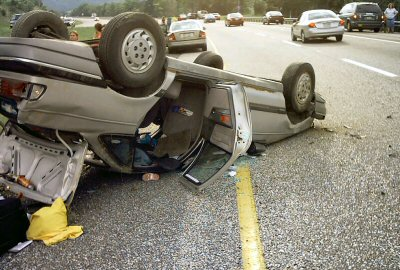
\includegraphics[scale=1]{pics/flip-over}
  \end{center}
  \item (車子)撞到了某處: \hilight{crash / bump / collide / run into ...}
\end{itemize}

\vspace{15mm}

\begin{center}
  \textbf{************ END OF THE DAY ************}
\end{center}

\newpage

\section{2016年1月18日 (Instructor: Vivian)}
\subsection{結核病}
\mybox{\centering \textbf{注意}: 本對話的更多筆記被歸納到專題里的關於``和疾病有關的詞", 請參考目錄進行查找!}
\subsubsection*{需要掌握的單詞短語}
\begin{multicols}{2}
\begin{itemize}
  \itemsep0em
  \item file: 資料, 病例\footnote{file這個詞在醫院有關的對話中不要翻譯成``檔案"!}
  \item 異常: abnormal ($adj.$) / abnormality ($n.$)
  \item 定期健康檢查: regular health checks
  \item 經常鍛鍊: regular exercise \hilight{(不要翻譯成定期鍛鍊)}
  \item 年齡的增長: \hilight{aging}, 可治癒的: \hilight{curable}
  \item 痰中帶血: blood \hilight{stained} sputum
  \item 盜汗: night sweating
  \item 慢性的 / 急性的: chronic / acute
  \item 驟然: in a short period
  \item 餐具: crockery
  \item 家用物品: Household items
\end{itemize}
\end{multicols}

\subsubsection*{需要掌握的句型}
\begin{itemize}
  \itemsep0em
  \item 沒什麼(特別的)問題: Nothing in particular.
  \item 我三周前開始咳嗽: I \hilight{have been coughing} since 3 weeks ago.
  \item 我體重突然下降: I have sudden weight loss.
  \item 這對嗎? \hilight{It is so?} / Is it right?
\end{itemize}

\subsubsection*{特別注意}
\begin{itemize}
  \itemsep0em
  \item 這篇文章出現了 sth. \hilight{and/or} sth. 翻譯時不要漏了其中一種情況. 
\end{itemize}

\subsection{醫療事故}
\subsubsection*{需要掌握的單詞短語}
\begin{multicols}{2}
\begin{itemize}
  \itemsep0em
  \item 手術器械: surgical utensil
  \item 醫療事故: medical incident
  \item 訴訟: lawsuit / litigation
  \item 提交(訴訟): lodge
  \item 當值律師: duty solicitor
  \item 法律程序: legal procedure
  \item 例行檢查: regular check-up
  \item 意向: preference (這裡不要翻譯成偏好)
  \item 照價賠償: pay agreed amount.
\end{itemize}
\end{multicols}

\subsubsection*{需要掌握的句型}
\begin{itemize}
  \itemsep0em
  \item 為這件事故感到沮喪: upset \hilight{over} this incident.
  \item 一大筆錢: large sum of money.
  \item 庭外和解: out of court settlement 或 settle the case / matter out of court.
  \item 幫助我庭外索賠: Help me with the claim / get the compensation outside the court.
\end{itemize}

\subsection{新移民}
\subsubsection*{需要掌握的單詞短語}
\begin{itemize}
  \itemsep0em
  \item 住址: \hilight{residential} address
  \item 好時機: good timing
  \item 優惠: concession
  \item 配偶移民: partner migration (scheme)
  \item TAFE (Technical and Further Education) 技術與繼續教育學院, 也可以不翻譯
\end{itemize}

\subsubsection*{需要掌握的句型}
\begin{itemize}
  \itemsep0em
  \item 我沒有別的選擇, 只能... : I don't have any other options, but to ...
\end{itemize}

\subsection{老年痴呆}
\subsubsection*{需要掌握的單詞短語}
\begin{multicols}{2}
\begin{itemize}
  \itemsep0em
  \item 婆婆: mother-in-law
  \item 阿茲海默症: Alzheimer's disease\footnote{阿茲海默症侵襲人的腦部;它並非正常的老化現象。得到阿茲海默症的人會漸漸的喪失記憶並且出現語言和情緒上的\\障礙。}
  \item 失憶症: amnesia
  \item 大小便失禁: incontinent
  \item (身體的)官能: faculty
  \item 幻覺: \hilight{hallucinations / delusion}
  \item 不安: restless
\end{itemize}
\end{multicols}

\subsubsection*{需要掌握的句型}
\begin{multicols}{2}
\begin{itemize}
  \itemsep0em
  \item 得了***病: has got ... = developed ...
  \item 不止這些: that's not all
  \item 尿床: wet someone's bed
  \item 坐不住: can't sit still
  \item 搓拉皮膚: rub and pull skin
  \item 怎麼可能: How could this be possible?
  \item 50多歲: in 50's.
  \item 身體壯得像頭牛: As tough as \hilight{nails}\footnote{不要直接把``牛"翻譯出來!}
  \item 並不常見: It is \hilight{not uncommon}.
\end{itemize}
\end{multicols}

\subsection{兒童發展}
\subsubsection*{需要掌握的單詞短語}
\begin{multicols}{2}
\begin{itemize}
  \itemsep0em
  \item 素質: potential
  \item 滿意: happy with\footnote{satisfy一般指比較大的生理或心理的滿足}
  \item 努力去做: struggle to do
  \item 阻礙以後發展: hold sb. back
  \item 一同參與: getting involved
  \item 健康障礙: physical barriers
\end{itemize}
\end{multicols}

\subsubsection*{需要掌握的句型}
\begin{itemize}
  \itemsep0em
  \item 他在學校表現如何: How is his performance at school?
  \item 在某人的這個年齡: someone of his / her age.
\end{itemize}

\vspace{15mm}

\begin{center}
  \textbf{************ END OF THE DAY ************}
\end{center}

\newpage

\section{2016年1月19日 (Instructor: Chris)}
\subsection{度假旅行}
\mybox{\centering \textbf{注意}: 本對話的更多筆記被歸納到專題里的關於``和暈車暈船有關的症狀", 請參考目錄進行查找!}
\subsubsection*{需要掌握的單詞短語}
\begin{itemize}
  \itemsep0em
  \item 旺季/淡季/平季: peak / off-peak / \hilight{shoulder} season
  \item 爬行動物: reptile
  \item 觀鯨旅遊: whale watching
  \begin{center}
    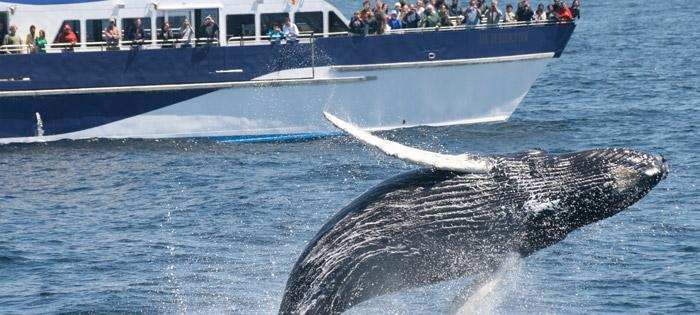
\includegraphics[scale=.5]{pics/whale-watching}
  \end{center}
  \item 假日套餐: holiday \hilight{packages},度假村: resort
  \item 近距離的: up close, 日光浴: sunbathing
  \item 暈動症: motion sickness
  \item 甲板: deck, 海上巡航: cruise
  \item 帶氧氣瓶潛水: Scuba diving, 浮潛: Snorkelling
  \item (旅遊)團: tour (不要翻譯成group)
  \item 舒活筋骨: stretch up
  \item 臨時預定: tentative booking
  \item 鞋架: shoe rack
\end{itemize}

\subsubsection*{需要掌握的句型}
\begin{itemize}
  \itemsep0em
  \item 靠海別墅: villa on the beach
  \item 也有道理: fair enough
  \item 措施機會(非意外): miss out on ...
\end{itemize}

\subsection{新移民資訊 (Hurstville)}
\mybox{\centering \textbf{注意}: 更多筆記被歸納到專題里的``和銀行有關的詞"和``宣傳冊和傳單", 請參考目錄查找!}
\subsubsection*{需要掌握的單詞短語}
\begin{itemize}
  \itemsep0em
  \item 公證件: \hilight{notarised} version (不是certified)
  \item Hurstville可以不翻譯!
\end{itemize}

\subsubsection*{需要掌握的句型}
\begin{itemize}
  \itemsep0em
  \item 本應該做但沒做: should have done ...
\end{itemize}

\subsection{支氣管炎}
\subsubsection*{需要掌握的單詞短語}
\begin{itemize}
  \itemsep0em
  \item 口水: saliva, (吐)痰: \hilight{(bring up)} sputum / phlegm
  \item 上氣不接下氣/氣短: short of breath
  \item 併發症: complications, 甲狀腺:thyroid gland (注意發音)
  \item 碘: iodine
  \begin{center}
    \includegraphics[scale=.7]{pics/iodine}
  \end{center}
  \item 肺炎: pneumonia, 青霉素: penicillin
  \begin{center}
    
\includegraphics[scale=.3]{pics/penicillin}
  \end{center}
  \item 乳製品: dairy products, 花粉: pollen, 粉塵: dust
  \item 撲熱息痛: paracetamol
  \item 抗組胺藥: antihistamine
  \item 安眠藥: sleeping pills
  \item 止疼藥: analgesic ($adj$ \& $noun$) / painkiller
  \item 粘稠的痰: \hilight{thick} sputum
  \item 黃綠色: \hilight{greenish yellow (其他顏色可以用類似方法表法, 注意調換順序)}
\end{itemize}

\subsubsection*{需要掌握的句型}
\begin{itemize}
  \itemsep0em
  \item 對...過敏: be allergic to...
  \item 以防萬一: for precaution / to be on the safe side
  \item 那時才發現: found back then
  \item 這可能是其中的原因嗎? Could it be the reason?
  \item 整個療程: full \hilight{course} of ...
  \item 高壓150, 低壓90: The blood pressure is 150 \hilight{over} 90.
\end{itemize}

\subsection{泌尿疾病}
\mybox{\centering \textbf{注意}: 本對話的更多筆記被歸納到專題里的關於``不同的疼法", 請參考目錄進行查找!}
\subsubsection*{需要掌握的單詞短語}
\begin{itemize}
  \itemsep0em
  \item 核磁共振: MRI (Magnetic Resonance Imaging)
  \item 尿道: Urinary tract
  \item 性病: Sexually Transmitted Diseases / Venereal Diseases
  \item 灼燒感: burning sensation
  \item 前列腺腫大: \hilight{enlarged} prostate
  \item (思想)開放: open / open-minded
  \item \hilight{空腹: fast}
  \item 頭巨痛: splitting headache
\end{itemize}

\subsubsection*{需要掌握的句型}
\begin{itemize}
  \itemsep0em
  \item 我每次排尿的時候都會感覺疼:
  \begin{enumerate}
    \itemsep0em
    \item It hurts everytime I pass water.
    \item It is painful everytime I pass urine. 
    \item I have pain everytime I pass water.
  \end{enumerate}
  \item 無意冒犯: no offence = with respect
  \item 你沒有冒犯到我: Not taken.
  \item 我不能忍受: I cannot bear / take / stand / put up with ...
\end{itemize}

\subsection{骨折(三級口譯)}
\mybox{\centering \textbf{注意}: 本對話的更多筆記被歸納到專題里的關於``不同的麻醉方式", 請參考目錄進行查找!}
\subsubsection*{需要掌握的單詞短語}
\begin{multicols}{2}
\begin{itemize}
  \itemsep0em
  \item 內部固定: Internal fixation
  \item 外部夾板: External splint
  \item 石膏拖: plaster cast
  \item 瘸著走路: walk with a limp
  \item 合適的急救: proper first aid.
  \item 大/小腿骨: thigh / calf bone
  \item 產假: maternity leave
  \item 事假: personal leave
  \item 喪假: funeral leave
  \item 長期服務假: long service leave
\end{itemize}
\end{multicols}

\vspace{15mm}

\begin{center}
  \textbf{************ END OF THE DAY ************}
\end{center}
\newpage

\section{2016年1月25日 (Instructor: Vivian)}
\subsection{就業幫助}
\subsubsection*{需要掌握的單詞短語}
\begin{itemize}
  \itemsep0em
  \item 非政府機構: Non-Government Organisation (NGO), 津貼: benefit / allowance
  \item 機械學: Machics, 機電維修: Mechanical \hilight{maintenance}, 機床廠: Machine tools / parts factory
  \item 偏僻的: isolated / remote
  \item 重拾自信: regain self-esteem, 自食其力: support themselves
  \item 個人\hilight{信息}: Personal \hilight{detail} (detail這裡不用翻譯成細節)
  \item 固定的 / 穩定的工作: Permanent employment (不要翻譯成永久的)
  \item (學歷)被承認: recognised
  \item 自卑: self-abased / self-inferior / low self-esteem
  \item 自我感覺良好(貶義): high self-esteem
\end{itemize}

\subsubsection*{需要掌握的句型}
\begin{itemize}
  \itemsep0em
  \item 我是(汽車)維修工: I'm a/an (auto) mechanic.
  \item 我想不明白...: I wonder why...
  \item 你讓我怎麼辦?:
  \begin{enumerate}
    \itemsep0em
    \item What else can I do?
    \item What do you expect me to do?
    \item What am I suppose to do?
  \end{enumerate}
  \item \hilight{省省吧, 不要說廢話: Just save it!}
  \item 配合某人走過場: Cooperate with sb. to \hilight{go through the formalities}.
  \item 在中國獲得的學歷: qualification obtained / acquired in China.
\end{itemize}

\subsubsection*{其他}
\begin{itemize}
  \itemsep0em
  \item ``學歷"翻譯成qualification, 學歷從低到高分別是 certificate, diploma和degree, 其中degree代表至少大學的學歷.
\end{itemize}

\subsection{種族歧視}
\subsubsection*{需要掌握的單詞短語}
\begin{itemize}
  \itemsep0em
  \item \hilight{背地裡: behind someone's back} (without a person's knowledge and in an unfair way.)
  \item 小舅子: brother-in-law
  \item 英文書: books in English
  \item 店主 / 店員: shop keeper / shop assistant, 白人: caucasian
  \item 出去: go out (走出去) / get out (滾出去, 用於罵人)
  \item 在場: at the scene
\end{itemize}

\subsubsection*{需要掌握的句型}
\begin{itemize}
  \itemsep0em
  \item 我收到了 / 遭受了歧視:
  \begin{enumerate}
    \itemsep0em
    \item I suffered discrimination.
    \item I was discriminated against...
    \item I was subjected to / a subject of discrimination.
  \end{enumerate}
  \item 拒絕為我服務: refuse to serve me
  \item 被視為: can be considered / regarded as
  \item 聽見有人背後說: I heard a voice behind.
  \item 聽了以後很不爽: I felt very uncomfortable after heard that.
  \item 回嘴:
  \begin{enumerate}
    \itemsep0em
    \item respond with a comeback.
    \item answer sb. back.
  \end{enumerate}
  \item 你怎麼認為的?: How did you take that?
  \item 依照種族背景: refer to ethnic background
  \item 目睹這個事情: Witness ($noun.$ + $verb.$, 這裡是動詞) the incident.
  \item 這是 / 那是我第一次做某事:
  \begin{enumerate}
    \itemsep0em
    \item This is my first time of doing something.
    \item That was the first time that I have done something.
  \end{enumerate}
\end{itemize}

\subsubsection*{其他}
\begin{itemize}
  \itemsep0em
  \item 歧視(discrimination) 一般有關於 gender / sexual, age 和 radial的
\end{itemize}

\subsection{人生低谷}
\subsubsection*{需要掌握的單詞短語}
\begin{itemize}
  \itemsep0em
  \item 搞砸: screwed up / mess up
  \item 苟延殘喘: keep struggle
  \item 自我形象: self image
  \item \hilight{潦而不倒: down but not out}
  \item \hilight{窮困潦倒: down and out}, 關於本俚語的來源和解釋請點\href{http://www.ept-xp.com/?ID=2204020903}{這裡}
\end{itemize}

\subsubsection*{需要掌握的句型}
\begin{itemize}
  \itemsep0em
  \item 我甚至不能...: I can't even managed to...
  \item 在我20多歲: In my 20's.
  \item 錯誤地歸咎: sb. wrongly blame sb. for sth.
  \item 照鏡子:
  \begin{enumerate}
    \itemsep0em
    \item I look into the mirror.
    \item I look at myself in mirror.
  \end{enumerate}
  \item 我還有救嗎: Do I have any hope?
\end{itemize}

\subsubsection*{其他}
\begin{itemize}
  \itemsep0em
  \item Overwhelm (壓倒性的):
  \begin{enumerate}
    \itemsep0em
    \item 太讓人受不了了: something is overwhelming.
    \item 被制服的, 被壓倒, 勢不可擋的: be overwhelmed.
  \end{enumerate}
\end{itemize}

\subsection{丟失包裹}
\mybox{\centering \textbf{注意}: 本對話的更多筆記被歸納到專題里的關於``正確表示地點" 和話外音里的``悉尼地名奇葩翻譯".}
\subsubsection*{需要掌握的單詞短語}
\begin{itemize}
  \itemsep0em
  \item 平郵 (陸地或海運輸) / 普通郵件: surface mail
\end{itemize}

\subsubsection*{需要掌握的句型}
\begin{itemize}
  \itemsep0em
  \item 我上海的一個親戚給我發了包裹: A relative of mine in Shanghai sent me a parcel.
  \item 不可能...: There is no way...
  \item 與我\hilight{短住}: \hilight{stay} at my place.
  \item 不可能把地址弄錯: There is no way he could have gotten the address wrong.
\end{itemize}

\subsection{社工訪談}
\mybox{\centering \textbf{注意}: 本對話的更多筆記被歸納到專題里的關於``不同的救助補貼", 請參考目錄進行查找!}
\subsubsection*{需要掌握的單詞短語}
\begin{itemize}
  \itemsep0em
  \item 社工訪談: Social worker interview
  \item 電焊的活 / 焊工: welding job / welder
  \item elaborate = explain in detail
  \item 經濟不景氣: economic depression / recession / downturn
  \item 天主教學校: Catholic (C大寫) school
  \item 房租補貼: rent \hilight{assistant}
  \item 輔助性的家庭津貼: supplementary family allowance
\end{itemize}

\subsubsection*{需要掌握的句型}
\begin{itemize}
  \itemsep0em
  \item 經濟拮據: experiencing / having a financial difficulty.
  \item 鬱悶的是: \hilight{What's upsetting} is that...
  \item 經濟突然不景氣: economy went down suddenly / \hilight{in a sudden}.
  \item 我被炒了魷魚: I was laid off / dismissed / \hilight{made redundant}
  \item 我的問題一個接著一個: I have had problems one after another.
  \item 攢錢買: save money to buy...
  \item 不能收支平衡: can't make ends meet
  \item 很高興能幫你: I'm glad I have been able to help ... (用於回答Thank you for helping me.)
\end{itemize}

\subsection{非法修剪樹木}
\subsubsection*{需要掌握的單詞短語}
\begin{itemize}
  \itemsep0em
  \item 美甲, 修腳: manicure, pedicure (都是$v.$ + $n.$)
  \item 砍: chop, 樹幹: trunk, 樹枝: branch
  \item 同意: consensus = consent
  \item 出庭: appear in / at court.
  \item 當地政府: local \hilight{council}
  \item 批准: approval / permit ($verb.$ + $noun.$) / permission
  \item 專業技術人員: tradesperson = skilled person
  \item \hilight{技術培訓: trades training}
  \item (身心)健康: well-being
  \item 漏看: overlook
\end{itemize}

\subsubsection*{需要掌握的句型}
\begin{itemize}
  \itemsep0em
  \item 莫名其妙: for no reason / without any reason.
  \item 因為某種原因: for some reasons.
  \item 有權力: be entitled to...
  \item 出庭: appear in / at court.
  \item 有一個關於你的訴訟: A lawsuit is being brought against you.
  \item 他收到一張傳票去\hilight{應訴} / 出庭作證: He has been served with a \hilight{subpoena} to \hilight{answer the charge in court} / \hilight{to give evidence in court}.
  \item 一張家庭暴力禁制令送達給某人(施暴的人): An apprehended domestic violence order has been \hilight{served} to sb.
  \item 又有什麼問題嗎??: What's wrong with that?? / Does it really matter?
  \item 反對: be opposed to / go against
  \item 英語說得比較好的朋友: Friend who speak \hilight{fairly} good English.
  \item 告某人:
  \begin{enumerate}
    \itemsep0em
    \item Sue $sb.$
    \item Take $sb.$ to court.
    \item Take legal action.
  \end{enumerate}
  \item 我的隔壁鄰居是個愛管閒事的人: My next-door neighbour is such a\hilight{nosy} person.
  \item 有權力: be entitled to...
\end{itemize}

\vspace{15mm}

\begin{center}
  \textbf{************ END OF THE DAY ************}
\end{center}

\newpage

\section{2016年1月28日 (Instructor: Chris)}
\subsection{毒品交易}
\mybox{\centering \textbf{注意}: 更多筆記被歸納到專題里的``和毒品有關的詞", 請參考目錄查找!}
\subsubsection*{需要掌握的單詞短語}
\begin{multicols}{2}
\begin{itemize}
  \itemsep0em
  \item 錄口供: make a statement
  \item 做筆錄: police interview
  \item \hilight{違法行為}: offense
  \item 酒保: bartender
  \begin{center}
    
\includegraphics[scale=0.3]{pics/bartender}
  \end{center}
  \item 挑釁: provoke ($v.$) / provocative ($adj.$)
  \item 攻擊性的, ``凶": aggressive
  \item 推責任: shift the blame / evade the responsibility\footnote{也可譯作``踢皮球"}
  \item 回憶, 記得: recollection $n.$
  \item 重新構思: reconstruction
  \item 黑手黨: Mafia
  \item 烈酒: spirit\footnote{注意和雪碧: Sprite 區分開!}
  \item 打火機, 火柴, : lighter / match
  \item 火把(火炬): torch
  \item 粗言穢語: abusive language
  \item 脾氣暴躁: grumpy
  \item 動手: start a fight / pick the fight\footnote{pick the fight不一定非是打, 也有可能是其他方式的衝突. 例句: I picked a fight \hilight{with} the guy beside me.}
  \item 同伴 (區別於friend): companions
  \item 搜身: frisk ($v.$)\footnote{例句: The passengers were frisked before they were allowed to board the plane. 俚語也可以譯作``扒竊".}
  \item 懸而未決的案子: cold case
\end{itemize}
\end{multicols}

\subsubsection*{需要掌握的句型}
\begin{itemize}
  \itemsep0em
  \item 我是被冤枉的: I'm innocent / \hilight{wronged}.
  \item 你一定要還我清白: You have to \hilight{clear my name}.
  \item 有人陷害我: I was set / framed by someone.
  \item 盡某人最大的能力: to the best of someone's ability
  \item 更別說: ... let alone / not to mention ... (不重要的放前面, 更重要的一些的放後面)\\例句: He is handsome and smart, not to mention being a good athlete.
  \item 趕走: take / escort\footnote{escort本身表示護送, 但依據上下文, 如果是被security guard護送, 則表示被趕走的意思.} someone out
  \item 例行公事: as a routine
  \item 有進展\hilight{第一時間}聯繫我: keep $sb.$ in the \hilight{loop} 或 keep $sb.$ updated / posted.
\end{itemize}

\subsection{尋求庇護者中心}
\subsubsection*{需要掌握的單詞短語}
\begin{multicols}{2}
\begin{itemize}
  \itemsep0em
  \item 尋求庇護者\footnote{尋求庇護者是指申請他國保護和居住權的人。尋求庇護者並不是難民。尋求庇護者並不是難民。如果因需要保護或其\\他原因,得到難民身份或居留許可,尋求庇護者便可在澳大利亞合法居留。} $\xrightarrow{\text{難民簽證下發}}$ 難民: asylum seeker $\xrightarrow{\text{refugee visa}}$ refugee
  \item 移民拘留中心\footnote{有關移民拘留中心的權利可參考: http://www.lawhelpny.org/files/B23B29BF-0DED-F7B9-2149-1DB14E1A7DE5/attachments/622E6AE2-F41B-C417-5DA5-6331ECC8BEDC/381307iamindetention.chi.pdf}: Immigration Detention Centre\footnote{被抓住的沒有合法簽證的人會被關押在這裡等待移民局對他們的claim / new application做出decision.}
  \item 移民與邊境保護事務部: Department of Immigration \& Border Protection
  \begin{center}
    
\includegraphics[scale=.6]{pics/dibp-logo}
  \end{center}
  \item 聯合國難民\hilight{公約}: UN Refugee Convention
  \item (非)人道: (in)humane 注意讀音!
  \item 迫害: persecution / persecute
  \item 移民復議仲裁庭: Migration Review Tribunal (主管臨時和永久簽證)
  \item 難民復議仲裁庭: Refugee Review Tribunal
  \item 口腔潰瘍: oral ulcer
  \item 刑法 / 民法: Criminal / Civil Law
  \item 刑法修正案: Criminal Law \hilight{Amendments}
  \item 簽署國: \hilight{signatory}
  \item 生活條件: living standard
  \item 消滅, 根除: wipe out
  \item 異議人士: dissident\footnote{如果考試時突然想不起這個詞, 可用``people with different political opinions"來``曲線救國"}
  \item 面對面的: \hilight{on-site} (有別於上門服務)
  \item 提供: provide $\xrightarrow{\text{變成名詞}}$ \hilight{provision} (of)
\end{itemize}
\end{multicols}

\subsubsection*{需要掌握的句型}
\begin{itemize}
  \itemsep0em
  \item 有錢能使鬼推磨: Money talks.
  \item 像罪犯一樣關起來: be locked up like a criminal.
  \item 我沒想到...: I don't expect...
  \item 最讓我擔心的是: What worries me most...
  \item 時不時: every now and then / from time to time
  \item 作為難民條約的簽署國: as a signatory \hilight{to} the Refugee Convention
\end{itemize}

\subsubsection*{注意}
請格外注意Reference中A5句的英翻中翻譯. ``on-site primary and holistic health care" 需要翻譯為``提供面對面的初級(基本)的和全面的健康保健", ``assistance with pharmaceutical costs" 翻譯成``藥物費用的補貼". ``pro bono dental" 翻譯成 ``慈善為目的的不收費的牙科服務". ``optical"不要理解成眼科, 需要翻譯成``視力的"(以配鏡為目的).

\subsection{移民後的困擾}
\mybox{\centering \textbf{注意}: 更多筆記被歸納到專題里的``和疾病有關的詞(三高)", 請參考目錄查找!}
\subsubsection*{需要掌握的單詞短語}
\begin{itemize}
  \itemsep0em
  \item 侄子 / 姪女: nephew / niece
  \item 假結婚: sham marriage
  \item 個案管理: case management
  \item 個人維權: \hilight{individual advocacy}
  \item (尿檢中的)中段尿: middle stage urine
  \item (尿液/血液) 樣本: \hilight{specimen} / sample
  \begin{center}
    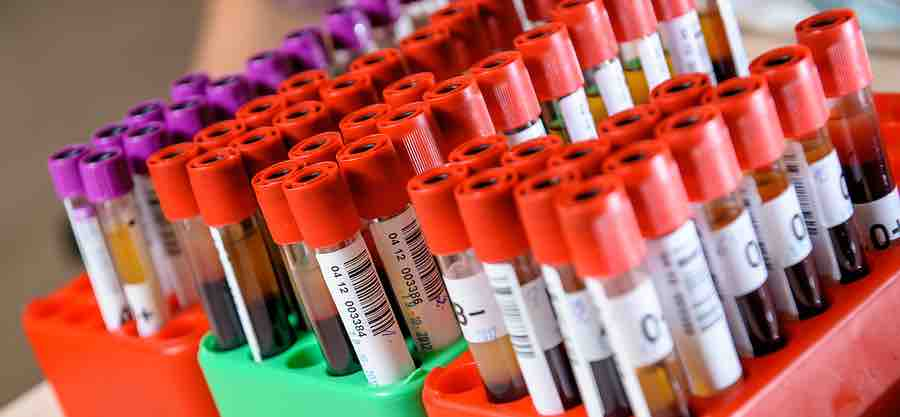
\includegraphics[scale=0.4]{pics/blood-sample}
  \end{center}
  \item 慈善的, 不收費的: pro bono (有別於free! 這個主要指以公共福利為目的)
\end{itemize}

\subsubsection*{需要掌握的句型}
\begin{itemize}
  \itemsep0em
  \item 靠帶來的一點錢過活: live on the money I brought here.
\end{itemize}

\subsection{簽證進度咨詢}
\mybox{\centering \textbf{注意}: 更多筆記被歸納到專題里的``和藍領職業有關的詞", 請參考目錄查找!}
\subsubsection*{需要掌握的單詞短語}
\begin{itemize}
  \itemsep0em
  \item 咨詢: enquire about...
  \item 提交(資料): submit / lodge / \hilight{file}
\end{itemize}

\subsubsection*{需要掌握的句型}
\begin{itemize}
  \itemsep0em
  \item 至今音訊全無: I haven't heard anything since.
  \item 做體檢: \hilight{take} the medical examination / check
  \item 身體好, 硬朗: \hilight{be in good shape / be physically fit}
\end{itemize}

\subsection{車禍賠償}
\mybox{\centering \textbf{注意}: 更多筆記被歸納到專題里的``不同的治療方式", 請參考目錄查找!}
\subsubsection*{需要掌握的單詞短語}
\begin{multicols}{2}
\begin{itemize}
  \itemsep0em
  \item 行車記錄儀: cam recorder
  \item 事務 / 文案律師: solicitor
  \item 巴律師 / 出庭大律師 (戴假髮) / ``大狀": barrister (also known as barrister-at-law)
  \item 人身傷害賠償金: Personal Injury \hilight{Damages}
  \item 激進的(療法): aggressive
  \item 五號公路: \hilight{M5} (M代表motoway)
  \item 丁字路口: T junction
  \item 車牌號: registration number
  \item 路口: intersection / junction / corner
  \item 兩個班次(工作): 2 shifts
  \item 過錯方: party \hilight{at} fault
  \item 判發, 發放: award
\end{itemize}
\end{multicols}

\subsubsection*{需要掌握的句型}
\begin{itemize}
  \itemsep0em
  \item 負責任且有能力的律師: a responsive and \hilight{capable} lawyer.
  \item 撞懵了: I froze (due to the crash).
  \item 腰很痛: sharp pain in my lower back.
  \item 誰有錯: Who was at fault?
  \item 撞向: collide into ...
  \item 直到開庭那天: up to the date of \hilight{hearing}.
  \item 遠遠不夠, 這哪裡夠: be far from enough
\end{itemize}

\subsection{腳踝和膝蓋受傷}
\mybox{\centering \textbf{注意}: 更多筆記被歸納到專題里的``不同的治療方式", 請參考目錄查找!}
\subsubsection*{需要掌握的單詞短語}
\begin{itemize}
  \itemsep0em
  \item 工傷賠償: Worker's Compensation (NAATI可接受簡稱comp, 也有簡稱compo)
  \item 工傷保險: Work Cover
  \item 倉庫: warehouse (主放商品存貨) / depot (t不發音)
  \item 骨科醫生: orthopaedist
  \item 骨外科, \hilight{矯形}外科: orthopaedic surgeon
  \item 狠狠摔: \hilight{nasty} fall
  \item 扭傷 / 拉傷: sprain / strain
  \item 不上班: off-work
  \item \hilight{way} more: ...多了 (相當於much more)
  \item 住房部: Department of Housing
\end{itemize}

\subsubsection*{需要掌握的句型}
\begin{itemize}
  \itemsep0em
  \item 我到單位後不久: Not long after I arrived at my workplace.
  \item 非常想知道: eager to know ...
\end{itemize}

\vspace{15mm}
\begin{center}
  \textbf{************ END OF THE DAY ************}
\end{center}
\chapter{醫學類 - Medical Dialogues}
\section{2016年2月1日 (Instructor: Vivian)}
\subsection{留學生抑鬱症}
\subsubsection*{需要掌握的單詞短語}
\begin{multicols}{2}
\begin{itemize}
  \itemsep0em
  \item 力氣: energy / strength
  \item 養活: support life
  \item 另一個自己: another me / self
  \item 離婚: divorce (及物動詞) divorce sb. (表示離婚的動作)
  \item 同父異母, 同母異父的兄弟: half brother
  \item 導致的原因: contributing factor
  \item 跟蹤: stalk / stalking
  \item 真理 / 真實存在的: true / real
  \item 大傷口 / 一條一條的傷: wound / cut
  \item 自殺: suicide (注意是名詞), 表示自殺動作: commit suicide
  \item 積蓄: savings
  \item 割腕: cut my wrist / wrist cutting
  \item 跳樓: jump off \hilight{a} building
  \item 傷心到崩潰: be devastated
  \item 雙重人格 / 人格分裂: dual personality / split personality
\end{itemize}
\end{multicols}

\subsubsection*{需要掌握的句型}
\begin{multicols}{2}
\begin{itemize}
  \itemsep0em
  \item 建議某人做某事: sb. suggests \hilight{I} do sth. / asks \hilight{me} to do sth.
  \item 向MRT遞交投訴: lodge an appeal \hilight{with} MRT.
  \item 履行...義務: fulfill one's obligation.
  \item 不是不...而是...: It's not that... (接主動句), but it's because / it's just...
  \item 更詳細地解釋: explain...in more detail
  \item 忍不住做某事: I can't help / stop doing sth.
  \item 和某人結婚 / 離婚: get divorced / married with sb 或 get a divorce with ...
  \item 自從...就...: Since..., has / have been doing sth.
  \item 被診斷出: be diagnosed with...
  \item 離開去工作: left for work
  \item ``知道以後"的兩種說法
  \begin{enumerate}
    \itemsep0em
    \item after I know (強調我一直都知道)
    \item after I get to know / find out (強調從不知道到知道)
  \end{enumerate}
  \item 讓某人喘不過氣: suffocate sb.
  \item 發洩出來: let it out
  \item 負能量爆棚: full of negative energy
  \item 堅持做某事
  \begin{enumerate}
    \itemsep0em
    \item Insist on sth. / doing sth.
    \item Insist that + 從句 (e.g. sb. should do sth.)
  \end{enumerate}
  \item 恢復了正常的意識: came to someone's senses.
  \item 讓...過去吧: let go of sth.
  \item 好好學習: do well in my studies.
\end{itemize}
\end{multicols}

\subsection{助聽器}
\subsubsection*{需要掌握的單詞短語}
\begin{itemize}
  \itemsep0em
  \item 助聽器: hearing aid
  \item 聽力 / 視力矯正師: Audiologist / Optometrist
  \item 聽覺神經: auditory nerves
  \item 高檔的診所: \hilight{fancy}\footnote{fancy不一定非要指外觀花哨} clinic
\end{itemize}

\subsubsection*{需要掌握的句型}
\begin{itemize}
  \itemsep0em
  \item 直接告訴我: tell me \hilight{straight up} (後面無逗號接陳述句)
  \item 我看不清圖: I can't \hilight{read} the graph.
  \item 情況更嚴重了:
  \begin{enumerate}
    \itemsep0em
    \item Condition gets serious / worse
    \item Worsens / Deteriorates
  \end{enumerate}
  \item 正視困難: face up the problem
  \item 資助某人: fund sb.
\end{itemize}

\subsection{鼻炎 (共三部分)}
\subsubsection*{需要掌握的單詞短語}
\begin{multicols}{2}
\begin{itemize}
  \itemsep0em
  \item 過敏反應: allergy reaction
  \item 鼻竇炎: sinusitis (簡稱sinus)
  \item \hilight{鼻炎: rhinitis}
  \item 過敏性 / 季節性鼻炎: allergic / seasonal rhinitis
  \item 小蟲咬的: insect bites
  \item 低燒: low grade fever
  \item \hilight{呼吸道: respiratory tract}
  \item 鼻塞: blocked / congested nose
  \item 十幾歲: in my \hilight{teens}
  \item 花粉 / 粉塵: pollen / dust
  \item 開花 / 花展: flowering / florae
  \item 異物: foreign material
  \item 威脅生命: \hilight{life-threatening}
  \item 呼吸道內壁: lining of the tract
  \item anaphylaxis = allergic reaction
  \item 營養不良: malnutrition
  \item 惡心: nauseous, nausea
  \item 化學氣味: chemical odour
  \item 乳糖: lactose
  \item 母乳: breastfeeding
  \item 流眼淚 / 鼻涕: streaming / watery eyes
  \item 流鼻涕: running nose
  \item 過敏源: allergens
\end{itemize}
\end{multicols}

\subsubsection*{需要掌握的句型}
\begin{multicols}{2}
\begin{itemize}
  \itemsep0em
  \item 她從來沒有得過(病): She has never had...
  \item 常見的小毛病:
  \begin{enumerate}
    \itemsep0em
    \item common ailment
    \item common minor illness
  \end{enumerate}
  \item 從...傳染的: got infected / caught / got it from...
  \item 引出...併發症: lead to / trigger / cause...
  \item 傳染性強的病毒性疾病: highly infected virus disease
  \item 不知什麼原因: for some reason
  \item 情況有所好轉: condition has improved / became batter.
  \item 我受夠他了: I am so fed up with sb.
\end{itemize}
\end{multicols}

\vspace{15mm}
\begin{center}
  \textbf{************ END OF THE DAY ************}
\end{center}
\newpage

\section{2016年2月2日 (Instructor: Chris)}
\subsection{肥胖症}
\subsubsection*{需要掌握的單詞短語}
\begin{multicols}{2}
\begin{itemize}
  \itemsep0em
  \item 避難所 / 安全島: refuge / refuge island
  \begin{center}
    
\includegraphics[scale=0.4]{pics/refuge-island}
  \end{center}
  \item 闖紅燈: run a red light (\hilight{run後面不加介詞})
  \begin{center}
    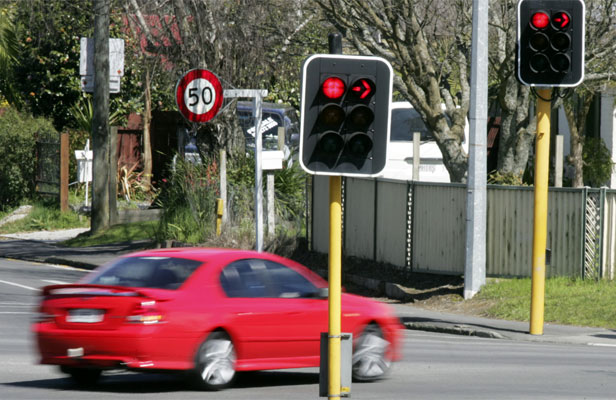
\includegraphics[scale=0.4]{pics/run-red-light}
  \end{center}
  \item 肥胖症: obesity ($n.$) / obese ($adj.$) 
  \item 心血管疾病: \hilight{cardiovascular} disease
  \item 體重指數: BMI (Body Mass Index)
  \begin{center}
    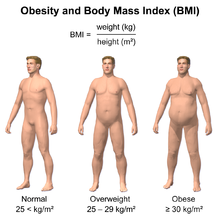
\includegraphics[scale=1]{pics/bmi}
  \end{center}
  \item 充血性心律衰竭: Congestive Heart \hilight{Failure} (failure在醫學里一般指\hilight{衰竭})
  \item 營養師: dietician / nutritionist
  \item 有氧運動: aerobics (一般30到40分鐘)
  \item 減肥藥: weight-loss pills
  \item 飲食配方: prescription diet
  \item 底線, ``關鍵是": bottom line
  \item 冥想: meditation
  \begin{center}
    
\includegraphics[scale=.3]{pics/meditation}
  \end{center}
  \item 規律: routine ($n.$ + $adj.$)
  \item energetic $\xrightarrow{\text{反義詞}}$ listless
  \item 暴食: binge eating
  \begin{center}
    
\includegraphics[scale=.3]{pics/binge-eating}
  \end{center}
  \item 碳水化合物: carbohydrate
\end{itemize}
\end{multicols}

\subsubsection*{需要掌握的句型}

\begin{itemize}
  \itemsep0em
  \item 少食多餐: eat more frequently but with less portion each meal.
  \item 我正想告訴你: I was going to tell you.
  \item 我稱了下體重: I \hilight{weighed} myself.
  \item stick to = keep doing...
  \item 量身定制...: It is tailored to...
  \item 試試: give / have a go / try
  \item 改善肥胖症:
  \begin{enumerate}
    \itemsep0em
    \item \hilight{improve} obesity
    \item recover from obesity
    \item treat obesity
  \end{enumerate}
  \item 與...一致/協調: in \hilight{tune} with...
  \item 往往: tend to...
\end{itemize}

\subsection{糖尿病}
\subsubsection*{需要掌握的單詞短語}
\begin{itemize}
  \itemsep0em
  \item 胰腺: pancreas $\xrightarrow{\text{分泌}}$ \hilight{insulin (胰島素)}
  \begin{center}
    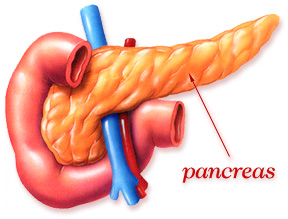
\includegraphics[scale=.5]{pics/pancreas}
  \end{center}
  \item 胰腺炎: pancreatitis
  \item impotence (陽痿) $\xrightarrow{\text{變成形容詞}}$ impotent \ \ \ \ \ \ \ \ frigidity (女性性冷淡) $\xrightarrow{\text{變成形容詞}}$ frigid
  \begin{center}
    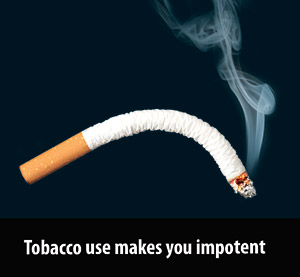
\includegraphics[scale=.6]{pics/impotence}
    
\includegraphics[scale=.45]{pics/frigidity}
  \end{center}
  \item 葡萄糖 / 甜食: glucose / sweets
  \begin{center}
    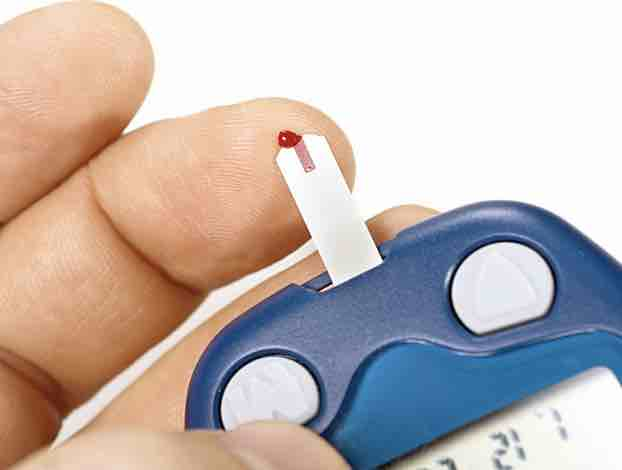
\includegraphics[scale=.2]{pics/glucose.jpg}
  \end{center}
  \item 內分泌科醫生: endocrinologist (endo代表內科, crino代表分泌)
  \item 截肢: amputation
  \item 飲食(表動作): dieting
  \item (血管中的)血流: bloodstream
\end{itemize}

\subsubsection*{需要掌握的句型}
\begin{itemize}
  \itemsep0em
  \item 喜食甜食者: have a sweet tooth \hilight{(tooth一定是單數)}.
  \item 堅持做某事: insist \hilight{on} doing sth / insist that + 從句.
  \item 您放心...: Let me reassure you...
  \item 我向您保證: Let me assure you...
  \item 徹底失明: lost someone's sight completely.
  \item 死於: \hilight{die of...(病) / die from...(天災人禍)}
  \item 非得這樣嗎?: Does it have to be the case?
\end{itemize}

\subsubsection*{其他}
\begin{itemize}
  \item 糖尿病的兩類:
  \begin{enumerate}
    \itemsep0em
    \item \textbf{Type I\footnote{1型糖尿病(舊稱青少年糖尿病或胰島素依賴型糖尿病)是糖尿病的一種類型,它與2型糖尿病的發病機理完全不同,屬於自體免疫性疾病,可能是基因或由於自體免疫系統破壞產生胰島素的胰腺胰島$\beta$細胞引起的,因此患者必須注射胰島素治療,目前世界上對此病沒有治癒方法。}} (genetic 先天的): insulin-dependent (胰島素依賴型)
    \item \textbf{Type II} (acquired 後天的): non-insulin dependent (非胰島素依賴型)
  \end{enumerate}
  \item 醫學里涉及的A, B, C, D在中文里要翻譯成\hilight{甲, 乙, 丙, 丁}.
  \item 廁所里看到的小箱子叫syringe disposal (註冊器丟棄), 一般用於insulin injection (胰島素注射).
  \begin{center}
    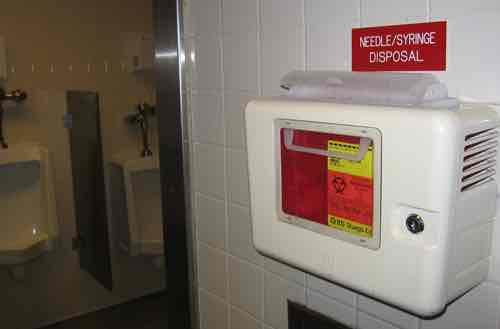
\includegraphics[scale=.6]{pics/syringe}
  \end{center}
\end{itemize}

\subsection{糖尿病檢查}
\mybox{\centering \textbf{注意}: 更多筆記被歸納到專題里的"人體的各種系統", 請參考目錄查找!}
\subsubsection*{需要掌握的單詞短語}
\begin{itemize}
  \itemsep0em
  \item (stress) echocardiogram: (負荷) 超聲波心動圖\footnote{超聲心動圖是應用超聲波回聲探查心臟和大血管以獲取有關信息的一組無創性檢查方法。包括M型超聲、二維超聲 、脈衝多普勒、連續多普勒、彩色多普勒血流顯像。}
  \item angiogram: 血管造影\footnote{血管造影是一種介入檢測方法,將顯影劑注入血管里,因為X光無法穿透顯影劑,血管造影正是利用這一特性,通過\\顯影劑在X光下所顯示的影像來診斷血管病變的。} (angio代表和血管有關)
  \begin{center}
    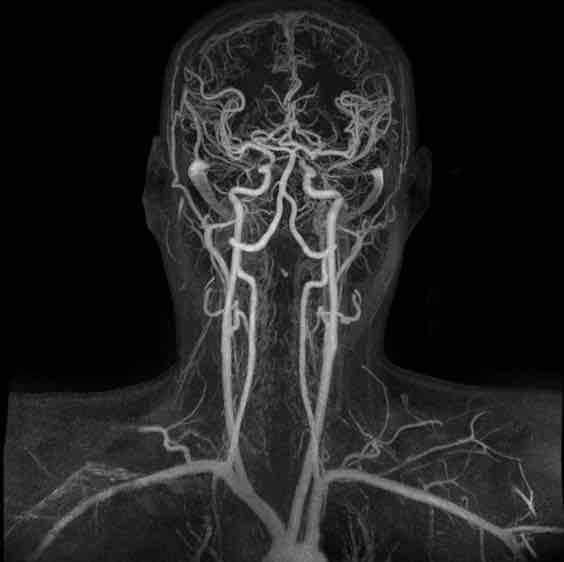
\includegraphics[scale=.3]{pics/angiogram}
  \end{center}
  \item 患妄想症的: paranoid $adj.$
  \item 惡化: deteriorate = get worse
  \item 劑量: dosage
  \item diabetes $\xrightarrow{\text{變成形容詞}}$ diabetic: $adj.$ 糖尿病的, $n.$ 糖尿病患者
  \item 癮: addiction
  \item 挫敗感: frustrated
  \item 人的三種血管: artery (動脈) / vein (靜脈) / capillary (毛細血管)
\end{itemize}

\subsection{針灸}
\subsubsection*{需要掌握的單詞短語}
\begin{itemize}
  \itemsep0em
  \item 針灸 / 針灸師: acupuncture / acupuncturist
  \item 手指:
  \begin{center}
    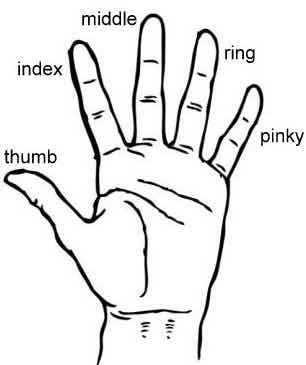
\includegraphics[scale=.55]{pics/fingers}
  \end{center}
  \item 穴位: acu-points
  \begin{center}
    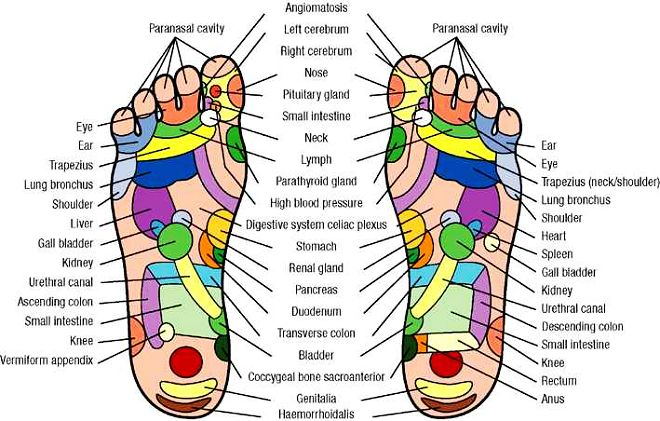
\includegraphics[scale=.75]{pics/acu-points}
  \end{center}
  \item 尼古丁貼劑: nicotine \hilight{patch} (patch還可以指膏藥)
  \begin{center}
    
\includegraphics[scale=.7]{pics/nicotine-patches}
  \end{center}
  \item 有決心 / 有毅力: determined / \hilight{dedicated}
  \item 免疫力: immunity
  \item 一根煙 / 一包煙 / 一條煙: a cigarette a smoke / a \hilight{pack} of cigarettes / a \hilight{carton} of cigarettes
  \item 生理慾望: craving
  \item 大煙槍: chain / heavy smoker
  \item 鎮靜: sedate ($\sim$ $sb.$) / sedation (put $sb.$ under $\sim$)
  \item 鎮靜劑: sedative (依然是\hilight{$n.$}) \hilight{重音在前}
  \item 麻痹感: numb ($adj.$) $\xrightarrow{\text{變成名詞}}$ numbness
  \item 揉: rub
  \item 膠帶: tape
  \item 耳朵的: auricular
  \item 神經末梢: nerve ends
  \item 中樞神經系統: Central Nervous System
\end{itemize}

\subsubsection*{需要掌握的句型}
\begin{itemize}
  \itemsep0em
  \item 減少吸煙量: reduce amount of cigarette
  \item 每天少吸五根煙: smoke five cigarettes less per day
\end{itemize}

\subsection{飲食紊亂}
\subsubsection*{需要掌握的單詞短語}
\begin{itemize}
  \itemsep0em
  \item anorexia (厭食症) $\xrightarrow{\text{反義詞}}$ bulimia (暴食症)
  \item 青春期少女: adolescent girl
  \begin{center}
    
\includegraphics[scale=.4]{pics/adolescent}
  \end{center}
  \item 習慣做某事: \hilight{get} used to...
  \item 皮包骨: skinny
  \item 油脂的, 油膩的: greasy
  \begin{center}
    
\includegraphics[scale=.5]{pics/greasy}
  \end{center}
  \item 反作用: \hilight{counter-productive}
  \item 兒童肥胖症: \hilight{childhood} obesity
\end{itemize}

\subsubsection*{需要掌握的句型}
\begin{itemize}
  \itemsep0em
  \item 少吃一頓飯: \hilight{skip} a meal
  \item 對...充耳不聞 / 視而不見: turn a deaf ear / blind eye to
  \item 體力活動變少: less physically active
  \item 讓某人明白: \hilight{get across to sb.} = make sb. understand
  \item 最好做: be better off doing sth.
\end{itemize}

\subsection{腸病}
\subsubsection*{需要掌握的單詞短語}
\begin{multicols}{2}
\begin{itemize}
  \itemsep0em
  \item 腹瀉: diarrhoea
  \item 腹痛: abdominal pain
  \item 腹脹: bloating
  \item 便秘: constipation
  \item 排便: bowel \textit{movement / motions / opening}
  \item 拉肚子: get the runs
  \item 不舒服: discomfort (不是un做前綴)
  \item colonoscopy: (結)腸鏡 (scopy代表醫用內窺鏡)
  \item 腸道易激綜合症: Irritable Bowel Syndrome\footnote{腸易激綜合徵(IBS)是一組持續或間歇發作,以腹痛、腹脹、排便習慣和(或)大便性狀改變為臨床表現,而缺乏胃\\腸道結構和生化異常的腸道功能紊亂性疾病。典型症狀為與排便異常相關的腹痛、腹脹,根據主要症狀分為:腹瀉主導型;\\便秘主導型;腹瀉便秘交替型。精神、飲食、寒冷等因素可誘使症狀復發或加重。}
  \item 非典型的: atypical
  \item 嚴重急性呼吸綜合症: Severe Acute Respiratory Syndrome (SARS) \footnote{是非典型肺炎的一種。中國簡稱為非典,根據英文發音有沙士、薩斯病、沙斯病或煞斯病等多種譯名。}
  \item 息肉 (polyp) $\xrightarrow{\text{惡性}}$ bowel cancer $\xrightarrow{\text{結腸}}$ colon cancer
  \item 輪流出現: alternative = take turns
  \item 篩查測試: \hilight{screening} test
  \item 化驗科, 病理學實驗室: pathology lab
  \item 排泄物潛隱血檢查: Fecal Occult Blood Test (FOBT) \footnote{糞便潛隱血(FOB)是指糞便中帶隱形血。糞便潛隱血測試通過將糞便塗抹於測試條進行檢查。}
\end{itemize}
\end{multicols}

\subsubsection*{需要掌握的句型}
\begin{itemize}
  \item 說(醫生用): complain of...
  \item ...藥讓...病好了幾天: The... stopped the ... for few days.
  \item 煙癮很大: smoke like a chimney
  \item 叫什麼來著: what is the word?
\end{itemize}

\vspace{15mm}
\begin{center}
  \textbf{************ END OF THE DAY ************}
\end{center}
\newpage

\section{2016年2月8日 (Instructor: Vivian)}
\begin{center}
  
\includegraphics[scale=.7]{pics/happy-year-2016}
\end{center}
\mybox{\centering \textbf{注意}: 今天上課的更多筆記被歸納到專題里的"身體部位和器官", 請參考目錄查找!}
\subsection{核磁共振}
\subsubsection*{需要掌握的單詞短語}
\begin{itemize}
  \itemsep0em
  \item 核磁共振: Magnetic Resonance Imaging (MRI)
  \item 蹲式廁所: squatting toilet
  \item 搬家: move / shift house
  \item (骨頭)復位: get it back / relocate the bone
  \item 潮濕天 / 下雨天: rainy day
  \item 軟組織\footnote{軟組織是指人體的皮膚、皮下組織、肌肉、肌腱、韌帶、關節囊、滑膜囊,神經、血管等。} : soft tissue
  \item 手鐲: bracelet
\end{itemize}

\subsubsection*{需要掌握的句型}
\begin{itemize}
  \itemsep0em
  \item 腿很酸: legs are sore
  \item 趕來: came in a hurry
  \item 沒當回事: didn't take is as a big deal / didn't take it seriously
\end{itemize}

\subsection{髖關節置換}
\subsubsection*{需要掌握的單詞短語}
\begin{multicols}{2}
\begin{itemize}
  \itemsep0em
  \item 髖關節置換: hip replacement
  \item 骨科醫生: orthopaedic surgeon
  \item 假體(肢): prosthesis
  \begin{center}
    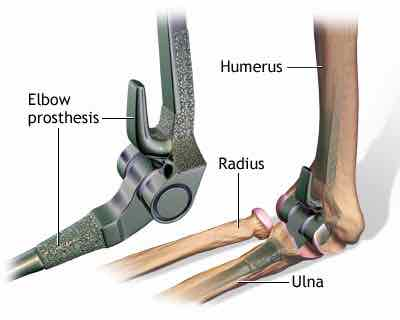
\includegraphics[scale=.5]{pics/prosthesis}
  \end{center}
  \item 消炎藥: anti-inflammatory
  \item 微創手術: minimally invasive surgery / key hole surgery
  \item 闌尾切除術: appendectomy (ectomy指...的手術)
  \item 心理準備: mentally prepared
  \item 主治醫生: attending doctor / attendings
  \item 大腿(根): thigh
  \item 血塊: blood clot
  \item 深靜脈血栓症: deep vein thrombosis
  \item 滑雪: skiing
  \item 私人醫生: private \hilight{health} insurance
  \item 自付費: out of pocket costs / expenses
  \item 最終決定: final say
\end{itemize}
\end{multicols}

\subsubsection*{需要掌握的句型}
\begin{itemize}
  \itemsep0em
  \item 做手術: perform the surgery / carry out the surgery
  \item 癱在床上: lie in bed paralysed
  \item 解釋怎麼做: explain how $sth.$ is done
  \item 新骨頭用什麼做的: What are the new bones made of?
  \item 關節磨損: wear and tear of joint (\hilight{worn表示磨損})
  \item 把...切除: have...removed
  \item 花...天恢復: It took me...days to recover.
  \item 請你注意: bear in mind
\end{itemize}

\subsection{哮喘發作}
\subsubsection*{需要掌握的單詞短語}
\begin{itemize}
  \itemsep0em
  \item 球場: pitch
  \item 上氣不接下氣: gasp for air
  \begin{center}
    
\includegraphics[scale=.3]{pics/gasp-for-air.jpg}
  \end{center}
  \item 預防性的藥物: preventative medications
  \item 支氣管擴張藥: bronchodilator agent (dilator指擴張劑)
  \item 對了, 說中了: Spot on!
  \item 四分之一決賽 / 半決賽 / 總決賽: quater-final /  semi-final / grand-final
  \item 我的疏忽: my own oversight
  \item (比賽的)隊長: captain
\end{itemize}

\subsubsection*{需要掌握的句型}
\begin{itemize}
  \itemsep0em
  \item 一開始慌神: I panicked at first.
  \item 謝謝關心: Thanks for caring.
  \item 突然, 無緣無故: out of the blue / out of sudden
  \item 你說對了: You got it spot on. / You hit the nail on the head!
  \item 不得不錯過: have to miss \hilight{out on}...
  \item 冒險去做: risk doing...
  \item 我還是...: I'd better...
\end{itemize}

\subsection{關節炎}
\subsubsection*{需要掌握的單詞短語}
\begin{itemize}
  \itemsep0em
  \item 風濕性 / 骨關節炎: rheumatic arthritis (維基百科查到rheumatoid arthritis) / osteoarthritis
  \item 老年病(專家): geriatric disease (geriatrics)
  \item 持續的疼: consistent pain, long-lasting pain
  \item 冰袋: icepack
  \item 減緩疼痛: kill / relieve / ease / alleviate the pain
  \item 遺傳缺陷: genetic predisposition
  \item 多補鈣: increase calcium intake
  \item 富含鈣: \hilight{rich} in calcium
  \item 耐力: endurance
\end{itemize}

\subsubsection*{需要掌握的句型}
\begin{itemize}
  \itemsep0em
  \item 在...大學讀書: study \hilight{at} ... university
  \item ...的原因是?: What are the causes of ...?
  \item (因為遺傳的)容易得某病: be predisposed to some disease
  \item 由...引起的: stem from...
  \item 當發作時吃止疼藥: take painkillers\footnote{服用painkiller的時候一般都是用複數} whenever it attacks / strikes / acts up
  \item 至於說...: as to...
  \item What should I pay attention to \hilight{in terms of} / \hilight{as to} my diet?
\end{itemize}

\subsection{高血壓}
\subsubsection*{需要掌握的單詞短語}
\begin{itemize}
  \itemsep0em
  \item 在晚年: in old age
  \item 遺傳性的疾病: genetic / hereditary / inherited disease
  \item 高膽固醇: high cholesterol
  \item 甲狀腺功能亢進症\footnote{甲狀腺功能活動過盛,甲狀腺激素分泌過多,其特徵是甲狀腺腫、心動過速或心房纖顫、脈壓增高、心悸、易疲勞、神\\經過敏和震顫、不耐熱、大量汗出、皮膚光滑濕熱、體重降低、肌肉虛弱、排便過多、情緒不穩以及眼部的症狀(如凝視、\\眼瞼遲滯、畏光,有時眼球突出)}: hyperthyroidism 
  \item 注意力不足過動症(多動症): Attention deficit hyperactivity disorder
  \item 重口味 / 輕口味食物: rich / plain flavour food
  \item 飲食習慣: eating habits
  \item 收縮壓 / 舒張壓: systolic / diastolic blood pressure (俗稱高低壓)
  \item 抗高血壓藥物: anti-hypertensive drugs
  \item 適量: in moderation
\end{itemize}

\subsection{肝炎}
\subsubsection*{需要掌握的單詞短語}
\begin{itemize}
  \itemsep0em
  \item 乙肝\footnote{又稱為血清性肝炎, 乙型病毒性肝炎, 是指乙肝病毒檢測為陽性, 病程超過半年或發病日期不明確而臨床有慢性肝炎表現者.} : hepatitis B
  \item 肝硬化: cirrhosis
  \item 感染病毒: catch the virus
  \item 餐具: eating utensils
  \item 接種: be vaccinated / get the vaccination
  \begin{center}
    
\includegraphics[scale=.7]{pics/vaccinated}
  \end{center}
\end{itemize}

\subsubsection*{需要掌握的句型}
\begin{itemize}
  \itemsep0em
  \item 電話里說...: tell $sth.$ \hilight{over} the phone
  \item 肝功能正常: Liver has been functioning properly.
  \item 和一般的驗血有區別嗎: Is it different to a general blood test?
\end{itemize}

\vspace{15mm}

\begin{center}
  \textbf{************ END OF THE DAY ************}
\end{center}

\newpage

\section{2016年2月9日 (Instructor: Chris)}
\mybox{\centering \textbf{注意}: 今天的更多內容請見詞彙專題里的Medicare詞彙!}
\subsection{皮膚癌}
\mybox{\centering \textbf{注意}: 本對話的更多內容請見詞彙專題里的``和皮膚病有關的詞"!}
\subsubsection*{需要掌握的單詞短語}
\begin{multicols}{3}
\begin{itemize}
  \itemsep0em
  \item 發生率: incidence
  \item 發病率: morbidity
  \item 死亡率: mortality
  \item 紫外線: UV rays
  \item 臭氧層: ozone layer
  \begin{center}
    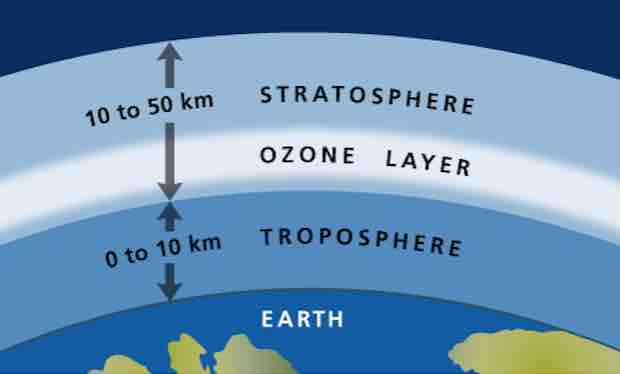
\includegraphics[scale=.25]{pics/ozone-layer}
  \end{center}
  \item 陽傘: parasol
  \item 防曬霜: sunscreen
  \item 防曬指數: Sun Protect Factor (SPF)
  \item 可防曬的衣服: protective clothing
  \item 太陽鏡: sunglasses (sunnies)
  \item 自由基\footnote{自由基, 係氧在體內新陳代謝後所產生的物質, 它的活性極強, 可與任何物質發生強烈的反應.}: free radical (加速皮膚老化)
  \item 活檢: biopsy\footnote{活體組織切片檢查}
  \item 中暑: sunstroke
  \item 曬傷: sunburn
  \begin{center}
    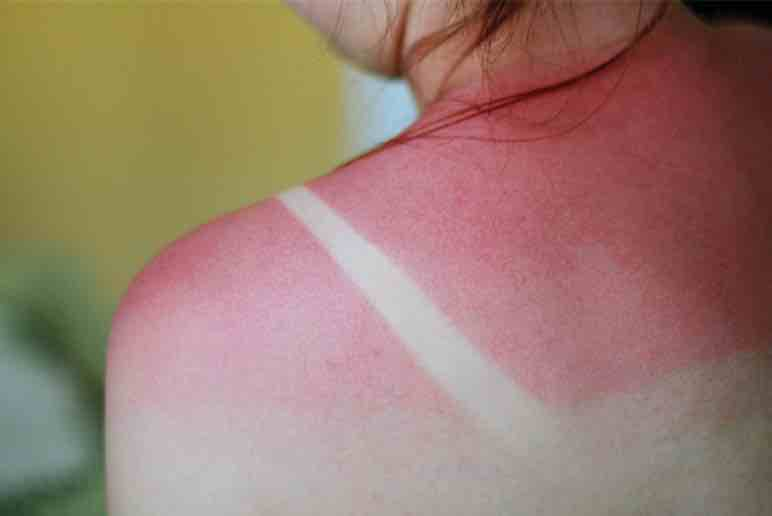
\includegraphics[scale=.2]{pics/sunburn}
  \end{center}
  \item outdoor = in the open air
  \item 暴露, \hilight{接觸}(輻射) = exposure
  \item 充足的防護: adequate protection
  \item 塗(防曬霜): apply
  \item 藥膏: cream ointment
  \item cure $vs.$ treat: 治癒 $vs.$ 治療
  \item 減少, 淘汰: eliminate
  \item 豬流感: \hilight{swine} flu
  \item 禽流感: \hilight{bird} flu
\end{itemize}
\end{multicols}

\subsubsection*{需要掌握的句型}
\begin{itemize}
  \itemsep0em
  \item 在我的手臂上: on my arm
\end{itemize}

\subsection{水痘 (共兩部分)}
\subsubsection*{需要掌握的單詞短語}
\begin{multicols}{2}
\begin{itemize}
  \itemsep0em
  \item body = trunk
  \item 低燒: mild fever
  \item 學徒: trainee
  \item 病毒性疾病: viral disease
  \item 火(爆)了: go viral
  \item 扇耳光: slap \hilight{in} face
  \item 肺炎 / 腦炎\footnote{腦炎是指腦實質受病原體侵襲導致的炎症性病變.}: pneumonia / encephalitis
  \item 爐甘石洗液: calamine lotion
  \begin{center}
    
\includegraphics[scale=.4]{pics/calamine-lotion}
  \end{center}
  \item 褥瘡: bedsore
  \begin{center}
    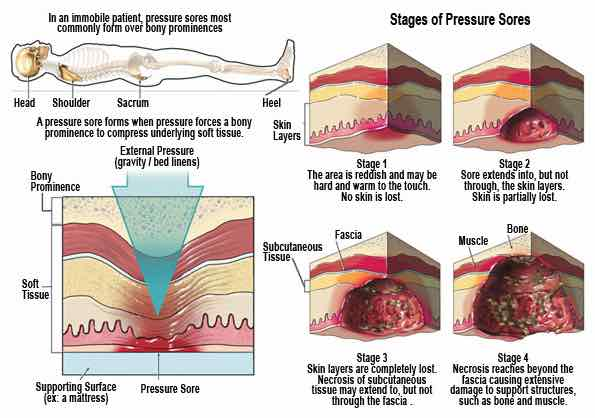
\includegraphics[scale=.4]{pics/bedsore}
  \end{center}
  \item 麻醉藥膏: anaesthetic cream
  \item 溫水 / 熱水 / 開水: \hilight{lukewarm} / warm / hot water
\end{itemize}
\end{multicols}

\subsubsection*{需要掌握的句型}
\begin{multicols}{2}
\begin{itemize}
  \itemsep0em
  \item 有一點發燒: A bit of temperature
  \item 我現在想起來: \hilight{Now that I come to think of it.}
  \item 與...相一致: be \hilight{consistent} with...
  \item 一定是被傳染: must have \hilight{contracted} / got / caught
  \item Chances are...: (放句首) 很有可能...
  \item ``一定一定": Most definitely / absolutely!
  \item 非常非常忙於: be overwhelmed by...
  \item 這也太煩了: What a nuisance! (nuisance單指心煩的事情)
  \item 生殖部位潰瘍: Sores in the \hilight{genital} area.
\end{itemize}
\end{multicols}

\subsection{丈夫不愛我了}
\subsubsection*{需要掌握的單詞短語}
\begin{itemize}
  \itemsep0em
  \item 讓我瘋了: drive me nuts / crazy
  \item 非常不開心, 感到痛苦的: distressing
  \item 出軌 / 出櫃: have an affair / come out of closet
  \item 各種家庭暴力的方式:
  \begin{enumerate}
    \itemsep0em
    \item 冷暴力: cold violence
    \item 情感上的折磨: emotional abuse
    \item 經濟上的\hilight{掌控}: financial abuse (在澳洲算家庭暴力)
    \item 言語辱罵: verbal abuse
    \item 性虐待: sexual abuse
    \item 虐待儿童: child abuse
    \begin{center}
      
\includegraphics[scale=.5]{pics/abuse}
      
\includegraphics[scale=.3]{pics/verbal-abuse}
    \end{center}
  \end{enumerate}
  \item 打(人): hit, beat, bash(狂揍)
  \item 揍了我一頓: beat me up
  \item 疏忽: oversight, negligence
\end{itemize}

\subsubsection*{需要掌握的句型}
\begin{multicols}{2}
\begin{itemize}
  \itemsep0em
  \item 這是一個友好的提醒: This is a \hilight{friendly / gentle} reminder that...
  \item 她被那些顾客辱骂: She's been abused by those customers.
  \item 無計可施, 束手無策:
  \begin{enumerate}
    \itemsep0em
    \item My hands are tied.
    \item I have no options.
    \item I have no way out.
  \end{enumerate}
  \item 大束玫瑰: A big bunches of roses.
  \item 最近才...: It is \hilight{only} recently that...
  \item 主動提出: offer to do...
  \item 值得一試: worth a try / shot / go
\end{itemize}
\end{multicols}

\subsubsection*{注意}
\begin{itemize}
  \item ``When he back home" 是錯誤的用法, 應該改成``When he comes back home".
\end{itemize}

\subsection{精神分裂症}
\subsubsection*{需要掌握的單詞短語}
\begin{multicols}{2}
\begin{itemize}
  \itemsep0em
  \item 精神分裂症: schizophrenia\footnote{Schizophrenia is a mental disorder characterized by abnormal social behavior and failure to recognize what is real.}
  \item 罵人: swear / yell \hilight{at} $sb.$
  \item 精神崩潰: mental breakdown
  \item 誓言: vow
  \item 睡得很死: deep sleep
  \item 認為(正式): perceive (perception 表示感知)
  \item 正經的, 得體的: decent $\xrightarrow{\text{反義}}$ indecent
  \item 同齡人: peers / people of his age
  \item 不睡覺: stay up (翻成``熬夜"即可)
  \item 問題男孩: difficult boy (難相處, 事情多, 老惹麻煩)
\end{itemize}
\end{multicols}

\subsubsection*{需要掌握的句型}
\begin{itemize}
  \itemsep0em
  \item 腦子不好使: \hilight{I can't think things clearly. / I can't think straight.}
  \item 累垮: \hilight{wear $sb.$ out.}
  \item 崩潰的邊緣: on the verge / edge of breakdown / collapse
  \item 他生病是因為...: He is sick in the sense that...
  \item 像我們這樣的正經家庭: decent family like ours
\end{itemize}

\subsubsection*{注意}
\begin{multicols}{2}
\begin{itemize}
  \itemsep0em
  \item lie / lied / lied 說謊
  \item lie / lay / lain 位於,躺
  \item lay / laid / laid: 置放, 鋪, 產 (蛋, 卵)
\end{itemize}
\end{multicols}

\subsection{疑似抑鬱的男孩}
\subsubsection*{需要掌握的單詞短語}
\begin{multicols}{2}
\begin{itemize}
  \itemsep0em
  \item 不情願: unwilling / reluctant ($adj.$)
  \item 小題大做: over-concerned
  \item 情緒低落: feel down
  \item 罪魁禍首: culprit
  \item 自卑: unconfident / self-abased
  \item 侮辱 / 羞辱: insult / humiliate
  \item 蔑視 / 嘲笑: contempt / tease
  \item 自殺傾向: suicidal tendency
  \item 遵守法律: observe the law
  \item 不開心的: low / down / gloomy / blue
\end{itemize}
\end{multicols}

\subsubsection*{需要掌握的句型}
\begin{multicols}{2}
\begin{itemize}
  \itemsep0em
  \item 他更不情願來了: He was more reluctant to come.
  \item 讓某人思想負擔過重: overburden of someone's mind.
  \item 看不起: look down upon...
  \item 假想出來的畫面: image from your assumption
  \item 被...發現: got caught by...
  \item 偶爾: once in a while
  \item 做某事是有道理的: have points in doing $sth.$
\end{itemize}
\end{multicols}

\vspace{15mm}

\begin{center}
  \textbf{************ END OF THE DAY ************}
\end{center}
\chapter{法律類}
\section{2016年2月15日 (Instructor: Vivian)}
\subsection{無證駕駛}
\subsubsection*{需要掌握的單詞短語}
\begin{itemize}
  \itemsep0em
  \item 疏忽駕駛 / 應照管的責任: driving without \hilight{due care} / duty of care
  \item 罰單 / 罰款: speeding \hilight{ticket} / penalty notice
  \begin{center}
    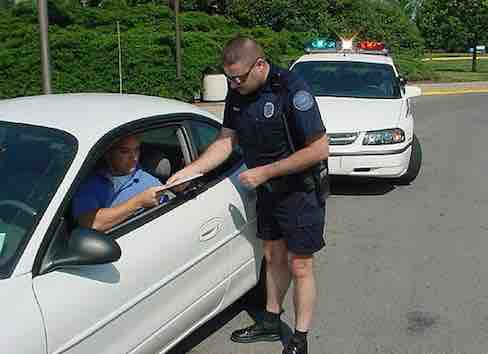
\includegraphics[scale=.5]{pics/speeding-ticket.jpg}
  \end{center}
  \item 駕駛執照: driver’s licence
  \item 臨時吊銷駕照 / 徹底吊銷駕照: \hilight{suspend} the licence / \hilight{revoke} the licence
  \item 疲勞駕駛 (的行為): fatigue driving 也可以譯作 \hilight{drowsy} driving / driving tired
  \item 超載: overload
  \item 罪犯, 違法 / 違章 / 違規者: offender (offence指違法行為)
  \item 違章: Road \& Traffic Offence
  \item PCA\footnote{詳情參考: \url{http://adamslawyers.com.au/prescribed-concentration-of-alcohol-and-drink-driving/}} : Prescribe Concentration of Alcohol (規定的酒精濃度)
  \item BAC: Blood Alcohol Content / Concentration (血液酒精濃度)
  \item RBT: Random Breath Test (隨機呼吸酒駕測試)
  \item (除酒外的)飲料: soft drinks / alcohol-free drinks
  \item 嚴重性: seriousness
  \item 委婉地謝絕(喝酒): decline (不用refuse或reject)
  \item 靠邊停車 / 把車開走: \hilight{pull over}  / pull out (也可以指突然發動車子)
  \begin{center}
    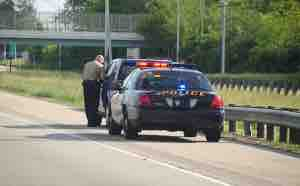
\includegraphics[scale=.7]{pics/pull-over}
  \end{center}
  \item 報名參加考試: register for the exam test
\end{itemize}

\subsubsection*{需要掌握的句型}
\begin{itemize}
  \itemsep0em
  \item She just arrived here / in Australia not long ago = She hasn’t been here very long.
  \item 我是一個奉公守法的人: I am a \hilight{law-abiding} person.
  \item 勸服: persuade sb. to do sth.
  \item 勸我喝酒: make me drink (urge sb. to do sth.)
  \item 我哪裡做錯了: Have I done anything wrong? / What have I done wrong?
  \item 把某人攔到一邊: \hilight{pull sb. over}
  \item 壓線行駛: straddle the \hilight{edge} of the lane
  \item 我知道是為什麼了: I see that’s why.
\end{itemize}

\subsection{跨道駕駛}
\subsubsection*{需要掌握的單詞短語}
\begin{itemize}
  \itemsep0em
  \item RTA: Road \& Traffic Authority 道路交通管理局\footnote{現在已經被合併到了Services NSW}
  \item 公路\hilight{海事}管理局: Road \& \hilight{Maritime} Service
  \begin{center}
    
\includegraphics[scale=.5]{pics/rms}
  \end{center}
  \item 正常的公路(非高速公路): highway
  \item 高速公路: freeway / express way / motorway
  \item 單子(一般指罰單): ticket / notice (但一般不說slip)
  \item 學習駕照: learner’s licence
  \item 全牌駕照 / 正式駕照: full licence
\end{itemize}

\subsubsection*{需要掌握的句型}
\begin{multicols}{2}
\begin{itemize}
  \itemsep0em
  \item Enquire about = make enquires about sth.
  \item 瞭解情況: get some information about…
  \item \hilight{當事人}都有誰: Who was involved?
  \item 事情的詳細經過是什麼: What happened exactly?
  \item 謝謝你能安排時間過來: Thank you for taking time to come.
  \item 我當時持有L牌: I was holding a learner’s licence.
  \item 我的駕駛技術不熟練: I am not a skilled driver.
  \item 在左右車道上: \hilight{in} the left / right lane
\end{itemize}
\end{multicols}

\subsubsection*{注意}
\begin{itemize}
  \itemsep0em
  \item 表達時間+日期:
  \begin{itemize}
    \itemsep0em
    \item It was at 8.30 in the morning, and on 30th of June.
    \item It was at 8.30 AM / PM \hilight{of} the 30th of June.
  \end{itemize}
  \item 當指``一個警察"的時候, 不要光說police, 要說\hilight{police officer}.
\end{itemize}

\subsection{家長會 (2015年12月11日真題)}
\subsubsection*{需要掌握的單詞短語}
\begin{multicols}{2}
\begin{itemize}
  \itemsep0em
  \item (在學校的)成績: academic performance
  \item 聽話: well behave
  \item \hilight{懂禮貌}, 尊敬別人的: respectful
  \item (課堂上)跟得上: catch up / keep up in class
  \item 鑒於 / 考慮到: given the fact…
  \item 家庭讀物: home reader
  \item 補習班: cram school (少用) / \hilight{coaching class} / tutoring class / coaching session
  \item (課上)認真聽講: concentrate in class
\end{itemize}
\end{multicols}

\subsubsection*{需要掌握的句型}
\begin{multicols}{2}
\begin{itemize}
  \itemsep0em
  \item 她聽話嗎: Has she be well-behaved?
  \item 在某方面幫助某人: help sb. with sth.
\end{itemize}
\end{multicols}

\subsubsection*{注意}
\begin{itemize}
  \itemsep0em
  \item Whether起頭的句子不是疑問句,  因此後面接的句子必須是陳述句語序.
\end{itemize}

\subsection{糖尿病 (2015年12月11日真題)}
\subsubsection*{需要掌握的單詞短語}
\begin{itemize}
  \itemsep0em
  \item (測量的)指標, 結果: reading
  \item 惡化: \hilight{deteriorate} / worsen
\end{itemize}

\subsubsection*{需要掌握的句型}
\begin{itemize}
  \itemsep0em
  \item 以防我忘記: in case I forget
  \item 最近視力模糊: my vision has been blurred recently
  \item 活不下去了: life is so hard
\end{itemize}

\subsubsection*{注意}
\begin{itemize}
  \itemsep0em
  \item 目前學過的虛擬語氣有兩種: I wish I had… 和 Should have done…
  \item \hilight{Since + 過去時 翻譯成``自從", Since + 完成時 翻譯成``因為"}
\end{itemize}

\subsection{法律咨詢(樓上夫妻吵架)}
\subsubsection*{需要掌握的單詞短語}
\begin{itemize}
  \itemsep0em
  \item 回想下: take back to (接時間 / 日期)
  \item 住在我們樓上 / 樓下的: live above / under us
  \item 吵架: argue
\end{itemize}

\subsubsection*{需要掌握的句型}
\begin{itemize}
  \itemsep0em
  \item 可能會出人命: someone's life might be in danger
  \item 無能為力: We couldn't help much.
\end{itemize}

\subsection{酒後駕車}
\subsubsection*{需要掌握的單詞短語}
\begin{multicols}{2}
\begin{itemize}
  \itemsep0em
  \item 聽證, 庭審: trail / court \hilight{hearing}
  \item \hilight{公訴人 / 公訴: prosecutor / prosecution}
  \item 減輕對我的處罰: reduce my punishment / impose a lenient penalty on me
  \item 網開一面 / 寬容: be lenient ($adj.$)
  \item 法官大人(稱呼): Your honour
  \item 巡邏警察: police on patrol
  \item (他們)老實點: behave themselves
  \item 酒醒了: \hilight{sober} ($adj.$)
  \item 一杯酒 / 牛奶: one glass of beer / milk
  \item 正當的 / 充分的理由: good reason
  \item 法庭的判決: court decision
  \item 付款 / 付清: pay / pay off
  \item \hilight{初犯: first time offender}
\end{itemize}
\end{multicols}

\subsubsection*{需要掌握的句型}
\begin{multicols}{2}
\begin{itemize}
  \itemsep0em
  \item 我(不)認罪: I plead (not) guilty.
  \item 用良好行為擔保: put $sb.$ on the good behaviour bond.
  \item 考慮: take $sth.$ into account / consideration
  \item 判你死刑: sentence you to death
  \item 我不是故意不配合: I didn't means to be uncooperative
  \item (方位)在我前面的人: the person in front of me
  \item 大大地影響收入: affect income greatly
  \item 真心的悔改: sincerely repentant
  \item 放我走: let me off
\end{itemize}
\end{multicols}

\subsection{駕駛執照 (第一部分)}
\subsubsection*{需要掌握的單詞短語}
\begin{itemize}
  \itemsep0em
  \item 分階段駕照制度: Graduated Licensing Scheme (Graduated 千萬不要翻譯成畢業生!)
  \item 臨時駕照: provisional licence (包括 Phase I / II (第一 / 第二階段))
  \item plate $\xrightarrow{\text{的人}}$ plater (翻譯成持有人, 等同於holder)
  \item 適合某人: suit someone's need
  \item 個人的需求: individual personal needs
  \item 和考駕照考試有關的詞:
  \begin{itemize}
  \itemsep0em
    \item 路況知識: knowledge about road
    \item \hilight{危險意識}測試: \hilight{Hazard Perception} Test
    \begin{center}
      
\includegraphics[scale=.5]{pics/hpt}
    \end{center}
    \item 駕駛員資格測試: Driver Qualification Test
    \item 機動車登記處: Motor Register
    \item 駕駛員知識測試: Driver Knowledge Test
  \end{itemize}
\end{itemize}

\subsubsection*{需要掌握的句型}
\begin{itemize}
  \itemsep0em
  \item 剛滿16週歲: just turned 16
  \item 這是我最大的顧慮: This is my biggest concern.
  \item \hilight{佔(比例): take up / account for}
  \item 從...過渡到: progress from ... to ...
  \item 一個較長的時間里: an extended period of time / over a period of time
  \item 同意某事: \hilight{be in favor of $sth.$}
  \item 把這個信息轉告他: \hilight{pass on} this information to him.
\end{itemize}

\subsection{駕駛執照 (第二部分)}
\subsubsection*{需要掌握的單詞短語}
\begin{multicols}{2}
\begin{itemize}
  \itemsep0em
  \item 交通法規 / 道路規章: road rule
  \item L牌(泛指): Ls
  \item clever (一般指小齡兒童) $\xrightarrow{\text{的人}}$ smart (指大一些的人)
  \item 方便, 好用: \hilight{handy} (This is an OZ expression)
  \item 規定的路線: set course
\end{itemize}
\end{multicols}

\subsubsection*{需要掌握的句型}
\begin{itemize}
  \itemsep0em
  \item 一次考過: pass the test \hilight{on the first try / in one go}
  \item L牌的有效期有多長?: How long is the learner's license valid for?
  \item 對他人的警覺: awareness of other
\end{itemize}

\vspace{15mm}

\begin{center}
  \textbf{************ END OF THE DAY ************}
\end{center}
\newpage

\section{2016年2月16日 (Instructor: Chris)}
\subsection{家庭暴力}
\mybox{\centering \textbf{注意}: 更多筆記被歸納到專題里的``澳洲不同的法院"和``各種打人的方式", 請參考目錄查找!}
\subsubsection*{需要掌握的單詞短語}
\begin{itemize}
  \itemsep0em
  \item 普外科\footnote{是以手術為主要方法治療肝臟, 膽道, 胰腺, 胃腸, 肛腸, 血管疾病, 甲狀腺和乳房的腫瘤及外傷等其它疾病的臨床學科}: general surgeon
  \item 流動測醉警車: booze bus
  \begin{center}
      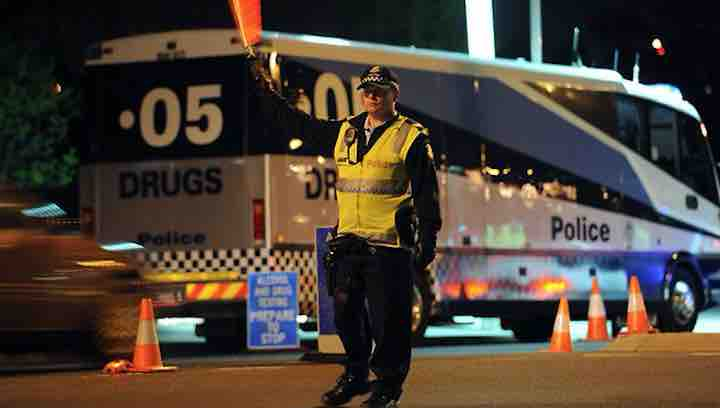
\includegraphics[scale=.5]{pics/booze-bus}
  \end{center}
  \item 酒駕整治行動: booze bus operation
  \item \hilight{Apprehended Violence Order (AVO): 暴力禁止令}
  \item Apprehended Domestic Violence Order (ADVO): 家庭暴力禁止令\footnote{適用於親戚, 同居關係甚至普通室友的關係}
  \item Apprehended Personal Order (APO): 個人禁止令
  \item 恐嚇 / 接近 / 跟蹤: intimidation / approach / stalk
  \item (高級)警員 / 警長(沙展) / 督查 / 警司: \hilight{(senior) constable} / sergeant / inspector / superintendent
  \item (警)問話, 筆錄: interview
  \item \hilight{嘮叨: nag (at)}\footnote{加不加at都可以}
  \item 奚落, 損, 嘲笑: taunt
  \item 打臉: hit \hilight{in} the face
  \item 鼻血: bleeding nose
  \item 頭暈 / 眩暈 / 偏頭痛 / 頭疼: dizziness / vertigo / migraine / headache
  \item 擋一下: block / \hilight{ward it off}
  \item 米蘭達規則: Miranda's Right\footnote{詳情請看 \url{https://www.legalzoom.com/articles/know-your-rights-what-are-miranda-rights}}
  \item 告誡卡\footnote{警察逮捕人時以防罪犯不懂英語, 將米蘭達告誡中文版印在卡上給罪犯看}: caution card
\end{itemize}

\subsubsection*{需要掌握的句型}
\begin{itemize}
  \itemsep0em
  \item 我們現在在說的這個問題: Now we are at it.
  \item \hilight{家醜不可外揚: We don't air the dirty laundry to the public.}
  \item 答到點子上了: answer to the point
  \item 煩死, 受夠某人: be sick (tired) of / be fed up with...
  \item 看不起: look down upon
  \item 你說我怎麼辦?!: You TELL ME what I should do.
  \item 有沒有搞錯?: Are you kidding me? / \hilight{Hello???} (注意語氣)
  \item 她怎麼打我的臉, 我就怎麼打回去: I hit her \hilight{the way} (way 可替換成 like how) she hit me in the face.
  \item 我真沒使這麼大力氣打她: I didn't hit her that hard.
\end{itemize}

\subsection{海關查獲 (第一部分)}
\subsubsection*{需要掌握的單詞短語}
\begin{multicols}{2}
\begin{itemize}
  \itemsep0em
  \item 犯法: breach (break) the law / do $sth.$ illegal / commit offence
  \item 出入境卡: Incoming Passenger Card / Outgoing Passenger Card
  \item 違禁物品: prohibited substances
  \item 行蹤, 下落(代替where): whereabout(s)
  \item 表姐: cousin
  \item 無意中聽到 / 偷聽: overhear / eavesdrop
  \item 欺負, 挑刺: bully / pick on...
  \item 檢疫(犬): \hilight{quarantine} (dog)
  \item 緝毒犬: sniffer dog
  \begin{center}
      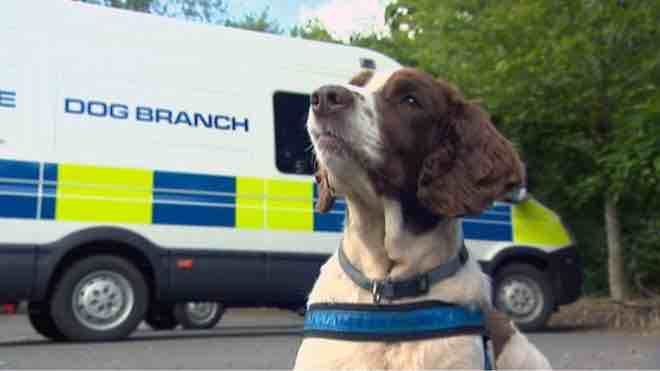
\includegraphics[scale=.3]{pics/sniffer-dog}
  \end{center}
  \item 家禽: poultry
  \item 植物成分: plant material
\end{itemize}
\end{multicols}

\subsubsection*{需要掌握的句型}
\begin{itemize}
  \itemsep0em
  \item 告誡某人: \hilight{caution $sb.$}
  \item 一定很擔心我: must be very worried about me.
  \item 如果你沒有家人在身邊: If you have no family around / by your side
\end{itemize}

\subsection{海關查獲 (第二部分)}
\mybox{\centering \textbf{注意}: 更多筆記被歸納到專題里的``各種法律懲罰", 請參考目錄查找!}
\subsubsection*{需要掌握的單詞短語}
\begin{itemize}
  \itemsep0em
  \item 重新開始, 繼續: resume
  \item \hilight{借進 / 借出: lend / borrow}
  \item (法律上的)說法: story (不要翻譯成故事)
\end{itemize}

\subsubsection*{需要掌握的句型}
\begin{itemize}
  \itemsep0em
  \item 越不想什麼, 越來什麼: The things I have got is what I need the least.
  \item 這是我最不想見到的: The thing I got is the last thing I want.
  \item 陷害某人: set $sb.$ up / frame $sb.$
\end{itemize}

\subsubsection*{其他}
\begin{itemize}
  \itemsep0em
  \item 米蘭達告誡: You have the right to remain silent. Anything you say can and will be used against you in a court of law. You have the right to talk to a lawyer and have him present while you are questioned. If you cannot afford to hire a lawyer, one will be appointed to represent you before questioning, if you wish one.
  \item 米蘭達告誡譯文: 你有權保持沈默,否則你所說的一切,都能夠、而且將會在法庭上作為指控你的不利證據;\\ 審問之前,你有權與律師談話,得到律師的幫助和建議;你受審問時你有權讓律師在場;\\ 如果你想聘請律師但卻負擔不起,法庭將為你指定一位律師.
\end{itemize}

\subsection{工傷賠償}
\subsubsection*{需要掌握的單詞短語}
\begin{multicols}{2}
\begin{itemize}
  \itemsep0em
  \item 工傷賠償: worker's comp / compo
  \item \hilight{工傷: worker-related injury}
  \item 工傷保險: Work Cover
  \item (全身)升降機: (full) body lifter
  \item \hilight{腰間盤突出: slipped disk(s)}
  \item 腰 / 腰圍: (lower) back / wrist
  \item 腦中風: stroke
  \item 中風病人: A stoke patient
  \item 上級的(護士): supervising nurse\footnote{大多數時候``上級"直接翻譯成supervisor即可.}
  \item 請假: take a leave / apply for a leave
  \item 用腰過度: \hilight{lumber muscle overstrain}\footnote{``曲線救國"的說法: overuse of lower back}
  \item 腰椎: lumbar vertebra (lumbar即是腰的形容詞)
  \item \hilight{康復: rehabilitation}
  \item 戒毒所: Rehabilitation Centre (簡稱\hilight{rehab})
  \item sort out = work out (整理)
  \item 肌肉勞損: Repetitive Strain Injury (RSI)
  \item 鏟車 / 叉車 / 堆高機: forklift
  \begin{center}
      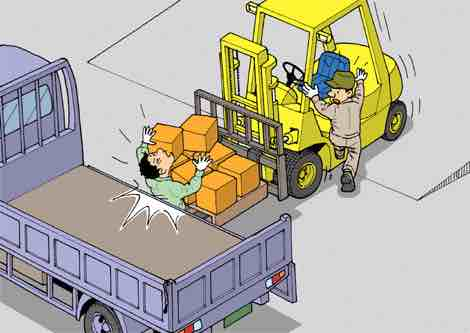
\includegraphics[scale=.3]{pics/forklift}
  \end{center}
  \item 裝貨 / 卸貨: load (unload)
  \item \hilight{倒車: reverse}
  \item 粉碎性骨折: \hilight{comminuted fracture}
  \item 間歇的: intermittent
\end{itemize}
\end{multicols}

\subsubsection*{需要掌握的句型}
\begin{itemize}
  \itemsep0em
  \item 在去年12月的中旬: in the mid of \hilight{last} December.
  \item 從...掉下來: fall \hilight{off from}...
  \item 劇烈的刺痛: sharp stabbing pain
\end{itemize}

\subsubsection*{注意}
\begin{itemize}
  \itemsep0em
  \item \hilight{請注意``months"的發音!!!}
  \item 不需要一直陪同的``送走"一般用send, 比如救護車把人送走, 但如果是朋友陪同去醫院, 一般用\hilight{``take $sb.$ to the hospital"}
  \item college 可與 workmate 互換
\end{itemize}

\subsection{侵犯隱私}
\subsubsection*{需要掌握的單詞短語}
\begin{multicols}{2}
\begin{itemize}
  \itemsep0em
  \item 惡意的: \hilight{malicious} / evil
  \item 理解: appreciate (這篇文章不翻譯成欣賞)
  \item 對律師的稱呼: Mr. / Ms. Solicitor
  \item 令人不安的: disturbing
  \item \hilight{晾衣服: air the laundry}
  \item 在二樓: on the second floor
  \item 灰色地帶: grey area
  \item 精神病患者, 變態: \hilight{psychopath}, phycho
  \item 色狼: pervert
  \item 確定: establish (這篇文章不翻譯成建立)
  \item 構成(犯罪): constitute
  \item 非法進入: trespass ($v.$ + $n.$)
\end{itemize}
\end{multicols}

\subsubsection*{需要掌握的句型}
\begin{multicols}{2}
\begin{itemize}
  \itemsep0em
  \item \hilight{好像: as if}
  \item 做不了什麼: do very little to...
  \item 我不敢: I don't dare
  \item 侵犯隱私: invasion / violation of privacy
  \item 讓陽光進來: let sunshine / daylight in
  \item 一樣 / 不亞於: no less than
  \item 告他賠錢: sue him for money
  \item (正)對準: point (directly) at...
  \item 而不是...: as oppose to...
  \item 在...的範圍內: within the bound of...
  \item 持續了一陣: over a substantiated period.
\end{itemize}
\end{multicols}

\vspace{15mm}

\begin{center}
  \textbf{************ END OF THE DAY ************}
\end{center}
\newpage

\section{2016年2月22日 (Instructor: Vivian)}
\subsection{遺囑}
\mybox{\centering \textbf{注意}: 更多內容請見法律詞彙專題里的和遗嘱有关的词!}
\subsubsection*{需要掌握的單詞短語}
\begin{multicols}{3}
\begin{itemize}
  \itemsep0em
  \item 報刊亭: news agency
  \item 修改, 修訂: amend ($v.$)
  \item 修正案: amendment ($n.$)
  \item 生孩子(重過程): give birth
  \item 指派, 委派: appoint / nominate
\end{itemize}
\end{multicols}

\subsubsection*{需要掌握的句型}
\begin{multicols}{2}
\begin{itemize}
  \itemsep0em
  \item 我不想鬧上法庭: I don't want to \hilight{end up in} court.
  \item 她剛生了小孩: She has just had baby.
  \item 遺產的比例: \hilight{share} of the estate
  \item 爭奪遺產: fight \hilight{over} estate.
  \item 強烈不建議:
  \begin{itemize}
    \itemsep0em
    \item strongly advise against doing sth.
    \item advise $sb.$ not to do.
\end{itemize}
  \item 關於: as to... / regarding...
  \item 按照你說的做: follow your \hilight{instructions}
\end{itemize}
\end{multicols}

\subsection{永久授權書}
\subsubsection*{需要掌握的單詞短語}
\begin{multicols}{2}
\begin{itemize}
  \itemsep0em
  \item 永久授權書: \hilight{enduring} power of attorney
  \item 代理人, 委託人: agent / attorney
  \item 授權人: principal / grantor / authoriser
  \item 起草: draft / draw up / prepare
\end{itemize}
\end{multicols}

\subsubsection*{需要掌握的句型}
\begin{multicols}{2}
\begin{itemize}
  \itemsep0em
  \item 這是怎麼弄的呢: How can it be done?
  \item 代理我行事: appoint $sb.$ to act on my behalf
  \item 管理: control \hilight{over} $sth.$
  \item 生效: come into effect / become effective / take effect
  \item 法律生效: come into force
  \item 弄完: have $sth.$ done / ready
\end{itemize}
\end{multicols}

\subsection{離婚事宜}
\subsubsection*{需要掌握的單詞短語}
\begin{multicols}{2}
\begin{itemize}
  \itemsep0em
  \item 孩子撫養權: child custody
  \item 孩子撫養費: child support (或maintenance)
  \item 配偶撫養費: alimony
  \item 監護權(不一定指離婚後): guardianship
  \item 孩子的探視權: access to child
  \item 撫養令 / 安排: parenting order / arrangement
  \item 復合, 重歸於好: get back together / reconciliation
  \item 提出離婚申請: lodge / apply for / file a divorce application
  \item 問題: question / \hilight{query}
  \item 審理(法律): hearing / trail
  \item 利益(法律): well-being
  \item 全部 / 共同撫養權: full / \hilight{joint} custody
\end{itemize}
\end{multicols}

\subsubsection*{需要掌握的句型}
\begin{multicols}{2}
\begin{itemize}
  \itemsep0em
  \item 和某人分居: separate \hilight{with} $sb.$
  \item 審理我的案子: hear my case
  \item 我們分居一旦滿12個月:
  \begin{itemize}
    \item \hilight{as soon as} we separate for 12 months.
    \item as soon as we meet the requirement of separating for 12 months.
  \end{itemize}
  \item 履行責任: \hilight{live up} one's responsibility  
  \item 達成協議: reach an agreement
  \item 定期: on a regular basis
\end{itemize}
\end{multicols}

\subsection{偷竊}
\subsubsection*{需要掌握的單詞短語}
\begin{multicols}{2}
\begin{itemize}
  \itemsep0em
  \item 一般違法行為: common \hilight{offence}
  \item 被扒了包: pick pocket / pocket picking
  \begin{center}
    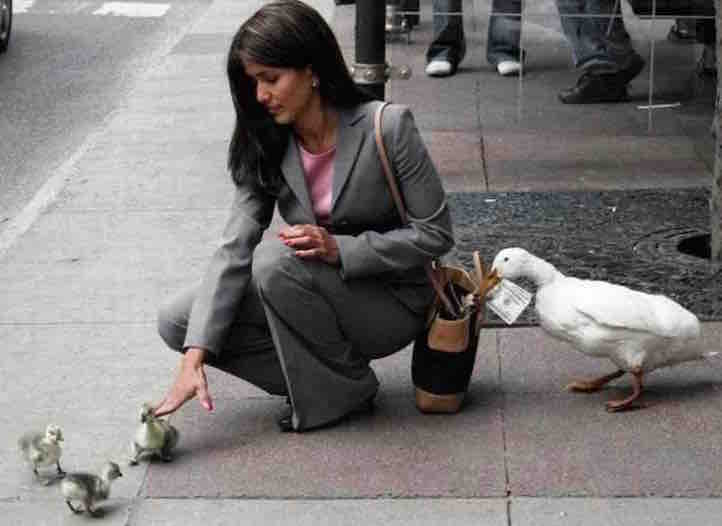
\includegraphics[scale=.3]{pics/pick-pocket}
  \end{center}
  \item 身份竊賊: identity theft
  \item 偷(不規則變化): steal / stole / stolen
  \item 貴重物品寄存處: valuables deposit box
  \item 小橫槓(``-"): hyphen
  \item 紀念品店: souvenir / gift shop
  \item 逛(商店): look around
  \item (物品)長得普通: plain-looking / average / ordinary
  \item 櫃台: counter
  \item 不在視線範圍: out of sight
  \item 單 / 雙肩包: satchel / backpack
\end{itemize}
\end{multicols}

\subsubsection*{需要掌握的句型}
\begin{multicols}{2}
\begin{itemize}
  \itemsep0em
  \item 我被扒了包: I have my pocket picked.
  \item 某物被偷走: steal $sth.$ away.
\end{itemize}
\end{multicols}

\subsection{便利店搶劫}
\subsubsection*{需要掌握的單詞短語}
\begin{multicols}{2}
\begin{itemize}
  \itemsep0em
  \item 錢櫃: till / register
  \item 初期調查: preliminary investigation
  \item 抓人: catch / capture (多指希望別人去抓)
  \item 混蛋: buster
  \item 有價值的線索: valuable leads
  \item 縮小(範圍): narrow down
  \item 嫌疑人範圍: suspect pool
  \item 犯罪現場調查小組: Crime \hilight{Scene} Investigation Team
  \begin{center}
    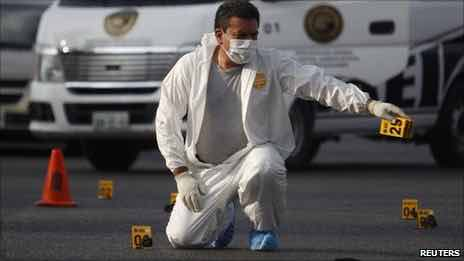
\includegraphics[scale=.48]{pics/csi-team}
  \end{center}
  \item 首要任務: priority, primary responsibility
  \item 裝修: renovation / refurbishment
  \item 破案: clear up / break / solve the case
\end{itemize}
\end{multicols}

\subsubsection*{需要掌握的句型}
\begin{multicols}{2}
\begin{itemize}
  \itemsep0em
  \item 另外兩個中的其中一個: one of the other two
  \item 這前後只有五分鐘: It all happened within 5 mins.
  \item 價值***的香煙: cigarettes \hilight{valued at} ***.
  \item 我從來沒想到這會發生在我身上: I didn't expect it would happen to me.
  \item 難道你們的首要任務不是保護市民的財產和安全嗎: Isn't protecting the property \& safety of the residents your primary responsibility? 
\end{itemize}
\end{multicols}

\subsection{商店盜竊}
\subsubsection*{需要掌握的單詞短語}
\begin{multicols}{2}
\begin{itemize}
  \itemsep0em
  \item 燭台: candle holder
  \item 尿布: nappy / diaper
  \item 嬰兒車: pram
  \item 公訴人: public prosecutor
  \item 監控錄像: security \hilight{footage}
  \begin{center}
    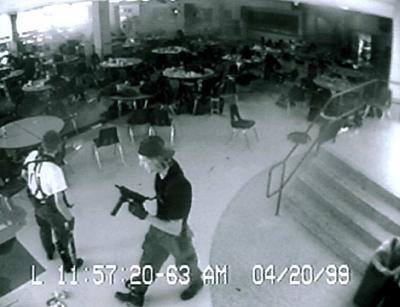
\includegraphics[scale=.55]{pics/security-footage}
  \end{center}
  \item 貨架: rack
  \item 兩個中的另外一個: the other
  \item 檢查(包): \hilight{inspect}, check
  \item 否認, 不配合(的態度): denial
  \item 人格擔保: character reference
  \item \hilight{誠實}: integrity
  \item 書面的證明證詞: testimony
\end{itemize}
\end{multicols}

\subsubsection*{需要掌握的句型}
\begin{multicols}{2}
\begin{itemize}
  \itemsep0em
  \item 移交給某人: pass $sth.$ to / onto $sb.$
  \item 被指控: be charged with...
  \item 他們冤枉我了: \hilight{They wronged me}.
  \item 看了錄像: have accessed to the security footage.
  \item 某事說不通: $sth.$ does not make sense.
  \item 證明某人的清白: prove my innocence
\end{itemize}
\end{multicols}

\vspace{15mm}

\begin{center}
  \textbf{************ END OF THE DAY ************}
\end{center}
\newpage

\section{2016年2月23日 (Instructor: Chris)}
\subsection{男朋友移民咨詢}
\mybox{\centering \textbf{注意}: 更多內容請見詞彙專題里的和澳洲移民相關簽證!}
\subsubsection*{需要掌握的單詞短語}
\begin{multicols}{2}
\begin{itemize}
  \itemsep0em
  \item 技術職業列表: Skilled Occupational List
  \item 職業評估: \hilight{Skill Assessment}
  \item 家庭團聚: family reunion
  \item 偏遠地區: \hilight{regional} area
  \item 雇主擔保: employer's sponsor
  \item 移民傾向: \hilight{tendency to migrate}
  \item 傾向, 目的: tendency / \hilight{inclination} / intention
  \item 間隔年: gap year\footnote{a gap year is a year before going to college or University and after finishing high school or taking a year off before going into graduate school after completing a bachelor as an undergraduate.}
  \item 事實婚姻關係: de facto relationship
\end{itemize}
\end{multicols}

\subsubsection*{需要掌握的句型}
\begin{multicols}{2}
\begin{itemize}
  \itemsep0em
  \item 讓我們回憶一下: \hilight{I take you back to + 日期}
  \item 徹底忘乾淨: throw $sth.$ out of the window
  \item 我怎麼會忘呢: How could I forget?
\end{itemize}
\end{multicols}

\subsubsection*{注意}
\begin{itemize}
  \itemsep0em
  \item Permanent Residency 一般代表政府發放的簽證, Permanent Residency 一般代表移民的狀態, 而Permanent Resident 只能指代拿到簽證的人.
  \item 可以瞭解一下澳洲常見簽證對應的編號, 這樣可以加速筆記, 具體可以參考話外音里的``澳大利亞簽證及其編號"!
\end{itemize}

\subsection{法庭交互式盤問}
\subsubsection*{需要掌握的單詞短語}
\begin{multicols}{2}
\begin{itemize}
  \itemsep0em
  \item 公平交易庭: Fair Trading
  \item 新州民事與行政仲裁庭: NCAT (NSW Civil and Administrative Tribunal)
  \item Fair Trading $\xrightarrow{\text{如果解決不了}}$ NCAT
  \item 調解: \hilight{conciliation / mediation}
  \item 調解員: conciliator / mediator
  \item 仲裁庭的仲裁員 / 仲裁官: member
  \item 攔下來: apprehend
  \item 嚇傻了: dumb-founded
  \item 文具: stationary
  \item 在特價 / 在打折: \hilight{on special} / discount
  \item 同等價值優惠券: rain check\footnote{原意: a ticket given for later use when a sporting fixture or other outdoor event is interrupted or postponed by rain.}
  \item 禮品註冊處(婚禮): gift registry
  \begin{center}
    
\includegraphics[scale=.4]{pics/gift-registry}
  \end{center}
  \item 專門放紅包的地方 (婚禮): wish well (也可以指許願池)
  \item 心不在焉, 腦子不在這: absent-minded
  \item \hilight{還}款付清: pay off
  \item 監控攝像頭: surveillance camera
  \item 監控錄像: surveillance footage
  \item (從被告席上)下來: stand down
  \item 有 / 無宗教信仰宣誓: oath\footnote{An oath is a verbal promise to tell the truth. Oaths are frequently made while holding the Bible, the New Testament or the Old Testament.} / affirmation\footnote{An affirmation is a verbal, solemn and formal declaration, which is made in place of an oath.}
\end{itemize}
\end{multicols}

\subsubsection*{需要掌握的句型}
\begin{multicols}{2}
\begin{itemize}
  \itemsep0em
  \item 讓我們回憶一下: I take you back to + 日期
  \item 徹底忘乾淨: throw $sth.$ out of the window
  \item 我怎麼會忘呢: How could I forget?
  \item 把商品臨時預定下來: put $sth.$ on layby
  \item 下次再去(表謝絕): take a raincheck?
  \item 過期不候: no rain check!
  \item 我這麼跟你說吧: I put it to you that...\footnote{言外之意: 我不信你所說的那些bullshit}
  \item 難道我被羞辱的還不夠嗎: Haven't I been humiliated more than enough?
  \item 讓某人出庭作證: put $sb.$ on the stand
  \item (法庭)我可以走了嗎: Can I be excused?
  \item (法庭)你可以走了: You can be excused.
\end{itemize}
\end{multicols}

\subsubsection*{注意}
\begin{itemize}
  \itemsep0em
  \item Don't you think 和 What if 後面要接陳述句!
\end{itemize}

\subsection{移民上訴仲裁庭}
\subsubsection*{需要掌握的單詞短語}
\begin{multicols}{2}
\begin{itemize}
  \itemsep0em
  \item 濕疹\footnote{濕疹是一種常見的過敏性皮膚病. 濕疹一詞通常泛指一系列持久和續發的皮疹, 以發紅, 水腫, 瘙癢和發乾為表徵, 可伴有結痂, 剝落, 起泡, 開裂, 出血或滲血.}: eczema
  \item 麻疹 / 蕁麻疹\footnote{蕁麻疹俗稱風團或風疹塊, 有的地區叫鬼風疙瘩, 中醫稱癮疹, 客語稱冷瘼, 是一種皮膚過敏. 症狀是局部皮膚忽然成塊地紅腫, 發癢, 幾小時後消退, 不留痕跡.} : measles / hives
  \item 風疹: German measles
  \item 不吃早飯: skip the breakfast
  \item 萬能的主: mighty god
  \item 有法律效力的, 有約束力的: binding
  \item 悶悶不樂: blue
  \item 不清醒的: \hilight{disoriented} / not clear-minded
\end{itemize}
\end{multicols}

\subsubsection*{需要掌握的句型}
\begin{multicols}{2}
\begin{itemize}
  \itemsep0em
  \item 是否還在: ... still there
\end{itemize}
\end{multicols}

\subsection{律師對話 - 家庭暴力禁止令}
\subsubsection*{需要掌握的單詞短語}
\begin{multicols}{2}
\begin{itemize}
  \itemsep0em
  \item 反社會人格: sociopath
  \item 沙包: punch bag
  \item (房門口的)腳墊: door mat
  \item 攻擊: assault
  \begin{center}
    
\includegraphics[scale=.6]{pics/assault}
  \end{center}
  \item 發洩: vent
  \item 酒醉鬼: alcoholic
  \begin{center}
    
\includegraphics[scale=.35]{pics/alcoholic}
  \end{center}
  \item 出路: \hilight{the way out}
  \item 八卦 / 謠傳: \hilight{gossip} / rumour
  \item 贍養費: maintenance
  \item 放棄: forgo
  \item 應得的財產: fair share
  \item 爭: fight over
  \item 眼鏡: spectacle
  \item 每天的折磨: \hilight{daily} torture
  \item 臨時判決書: decree nisi
  \item 最終判決書: decree absolute
  \item 達成和解: reach a reconciliation
\end{itemize}
\end{multicols}

\subsubsection*{需要掌握的句型}
\begin{multicols}{2}
\begin{itemize}
  \itemsep0em
  \item 與某人相處: get along with ...
  \item 喝醉酒回家: \hilight{come home drunk}
  \item (輕)打屁股: spank the bottom
  \item 忍受: \hilight{put up with...}
  \item 進而看下一步: take it from there.
  \item 出洋相: to make a spectacle of oneself
  \item 把某人當出氣筒: \hilight{treat $sb.$ as punch bag / door mat}
  \item 拿某人出氣: \hilight{vent} / take it out on $sb.$
\end{itemize}
\end{multicols}

\subsection{法律咨詢 - 家庭暴力禁止令}
\subsubsection*{需要掌握的單詞短語}
\begin{multicols}{2}
\begin{itemize}
  \itemsep0em
  \item 工作人員: support officer
  \item 列出: set out = list
  \item 暴怒: furious (with $sb.$)
  \item 違反(法律): breach
  \item 淤青: bruise
  \item 發紅: redness
  \item 血痕: blood stain
  \item 疤 / 痂: scar / scab
  \item 青一塊紫一塊: black and blue
\end{itemize}
\end{multicols}

\subsubsection*{需要掌握的句型}
\begin{multicols}{2}
\begin{itemize}
  \itemsep0em
  \item 渾然不知, 不知所措: be confused and at a loss.
  \item 關在監獄: be locked up in jail / gaol
  \item 在中國沒有這回事: there is no such thing in China.
  \item 求助於某人: turn to $sb.$ (for help)
\end{itemize}
\end{multicols}

\subsection{家庭暴力 - 干涉令}
\subsubsection*{需要掌握的單詞短語}
\begin{multicols}{2}
\begin{itemize}
  \itemsep0em
  \item 報復: revenge / get back \hilight{at}
  \item (法律文件)起效力: in force
  \item 安全感: sense of security
  \item 遵紀守法: law-abiding
\end{itemize}
\end{multicols}

\subsubsection*{需要掌握的句型}
\begin{multicols}{2}
\begin{itemize}
  \itemsep0em
  \item 送達: be served on...
\end{itemize}
\end{multicols}

\vspace{15mm}

\begin{center}
  \textbf{************ END OF THE DAY ************}
\end{center}
\newpage
\chapter{雜類話題II}
\section{2016年2月29日 (Instructor: Vivian)}
\subsection{立遺囑}
\mybox{\centering \textbf{注意}: 更多內容請見法律詞彙專題里的和遺囑有關的詞!}
\subsubsection*{需要掌握的單詞短語}
\begin{multicols}{2}
\begin{itemize}
  \itemsep0em
  \item 遺漏, 錯過機會: miss out
  \item 房產, 財產: property\footnote{property這個詞需要根據上下文來確定如何進行翻譯!}
  \item 資產: assets
  \item 遺產: estate
  \item 廢除: \hilight{revoke}
  \item 所有物: possessions
  \item 佔有欲: possessive
  \item 銀行存款: bank savings
  \item 自己存的退休金: \hilight{superannuation}
  \item 政府撫卹發放的養老金: pension
  \item 免除, \hilight{一筆勾銷}: be forgiven
  \item 被繼承: be inherited
  \item 健在的家庭成員: surviving family member
  \item 財產的繼承人: heirs to the property
  \item 個人債務: personal debts
  \item 值得信賴的: \hilight{trustworthy}
  \item 個人情況: personal circumstances
\end{itemize}
\end{multicols}

\subsubsection*{需要掌握的句型}
\begin{itemize}
  \itemsep0em
  \item 我想知道: I wander... (盡量少用, 這個表請求的語氣)
  \item 問區別:
  \begin{itemize}
  \itemsep0em
  	\item Is there a difference between doing A and (doing) B?
  	\item Does it make a difference if I do A or do B?
  	\item ...if one dies with or without a will?
  \end{itemize}
  \item 我的遺囑什麼時候可以生效:
  \begin{itemize}
  \itemsep0em
  	\item How can my will come into effect?
  	\item How can I make my will come into valid?
  \end{itemize}
  \item 遺囑里應該包含什麼:
  \begin{itemize}
  \itemsep0em
  	\item What should I include in my will?
  	\item What should be included in a will?
  \end{itemize}
  \item 通過遺囑檢驗獲批來生效: put into effect by a grant of probate.
  \item 以書面, 有簽字並見證的(方式): be in writing, signed and witnessed.
  \item 我對...有...的股份: of which / in which I hold...of the shares.
  \item 可能有責任承擔(法律責任): may be (held) liable for $sth.$ / to do...
  \item \hilight{貸款: take out a loan / mortgage}
  \item \hilight{資金週轉(不靈): cash / capital flow (difficulties)}
  \item 這樣是為了...: so as to do...
  \item 考慮做某事: consider doing...
  \item 對我有幫助: helpful to me
  \item 幫了我大忙了:
  \begin{itemize}
  \itemsep0em
  	\item It has helped me a lot!
  	\item It has been really helpful!
  \end{itemize}
\end{itemize}

\subsection{減肥}
\subsubsection*{需要掌握的單詞短語}
\begin{multicols}{2}
\begin{itemize}
  \itemsep0em
  \item 迭縫帶環: lap-band (surgery)\footnote{an inflatable silicone device placed around the top portion of the stomach to treat obesity, intended to slow consumption of food and thus reduce the amount of food consumed.}
  \begin{center}
  	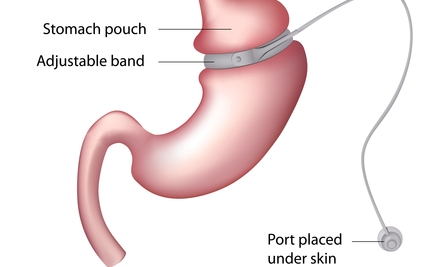
\includegraphics[scale=1.8]{pics/lap-band}
  \end{center}
  \item 脂肪抽吸手術, 抽脂術: liposuction\footnote{Areas affected can range from the abdomen, thighs and buttocks, to the neck, backs of the arms and elsewhere.}
  \item 肥胖症患者: \hilight{obese patient}
  \item 新陳代謝: \hilight{metabolism}
  \item 減肥藥: weight-loss pill
  \item 便秘的: constipated
  \item 壓迫: stain
  \item 減肥: \hilight{shape up / slim down}
  \item 高膽固醇: high \hilight{cholesterol}
  \item 高脂肪食物: \hilight{fatty foods}
  \item 心絞痛: angina
  \item 蔬菜和水果: fruit and vegetable\footnote{在英語中蔬菜水果的位置要顛倒}
\end{itemize}
\end{multicols}

\subsubsection*{需要掌握的句型}
\begin{multicols}{2}
\begin{itemize}
  \itemsep0em
  \item 我覺得疼
  \begin{itemize}
  \itemsep0em
  	\item I am \hilight{in pain}.\footnote{建議用這個, 既可以表示生理, 也可以表示心理.}
  	\item I feel pain in...
  	\item There is a pain in...
  \end{itemize}
  \item 疼得很厲害
  \begin{itemize}
  \itemsep0em
  	\item \hilight{unbearable pain}
  	\item Pain is killing me.
  \end{itemize}
  \item 促進新陳代謝: \hilight{increase metabolism}
  \item 負擔不起風險: \hilight{afford} to take such risk
  \item 一一對應: \hilight{match $sth.$ with $sth.$}
  \item 不介意做: I don't mind doing $sth.$
  \item 我只好: I have no choice but...
  \item 節食: be on a diet
\end{itemize}
\end{multicols}

\subsection{酒駕}
\subsubsection*{需要掌握的單詞短語}
\begin{multicols}{3}
\begin{itemize}
  \itemsep0em
  \item 零點零七: 0.07 / \hilight{.07}\footnote{在對話中可能.之前的零不會讀出來, 要格外注意!}
  \item 讀數: reading
  \item 初犯: \hilight{first time offender}
  \item 從輕處罰: reduce the punishment
  \item 罰我錢: fine me\footnote{fine在這裡做$v.$}
  \item 罰單: penalty notice
  \item 照章辦事: follow the rule
  \item 嚴厲: \hilight{harsh}\footnote{可以和punishment搭配}
  \item 沒氣, 沒電: flat
\end{itemize}
\end{multicols}

\subsubsection*{需要掌握的句型}
\begin{multicols}{2}
\begin{itemize}
  \itemsep0em
  \item 為什麼只攔下我呢: Why did you only stop me?
  \begin{center}
  	
\includegraphics[scale=.4]{pics/stop-me}
  \end{center}
  \item 勸人喝酒: persuade / make $sb.$ to drink
  \item \hilight{屬於是}: falls into / within...
  \item 電池沒電了:
  \begin{itemize}
  \itemsep0em
  	\item The battery is dying.
  	\item The battery is flat.
  	\item I have run out of battery.
  \end{itemize}
\end{itemize}
\end{multicols}

\subsection{骨質疏鬆症}
\subsubsection*{需要掌握的單詞短語}
\begin{multicols}{2}
\begin{itemize}
  \itemsep0em
  \item 骨質疏鬆症: \hilight{osteoporosis}\footnote{骨質疏鬆症是一種鈣質由骨骼往血液淨移動的礦物質流失(demineralization)現象,骨質量減少,骨骼內孔隙增大,呈現中空疏鬆現象,速率取決於破骨細胞(osteoclast)和成骨細胞(osteoblast)活性的消長。此需和軟骨症(osteomalacia)有所區別,軟骨症的成因是維生素D的缺乏所導致。}
  \begin{center}
  	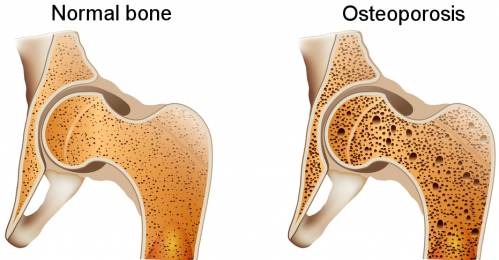
\includegraphics[scale=.5]{pics/osteoporotic}
  \end{center}
  \item 腰疼: lumbago = lower back pain
  \item 腰椎間盤: \hilight{lumbar discs}
  \item ...誘發的: \hilight{...-induced}
  \item 脊椎骨裂: fractures\footnote{這裡不要翻譯成骨折, 否則顯得很嚴重} in the spine
  \item 無症狀的: asymptomatic
  \item 止痛貼: analgesic patch
\end{itemize}
\end{multicols}

\subsubsection*{需要掌握的句型}
\begin{multicols}{2}
\begin{itemize}
  \itemsep0em
  \item 腰疼還是老樣子: lower back pain \hilight{remains the same}.
  \item 讓我做...測試: order...test for me
  \item 更容易患上...: be more susceptible to $sth.$
  \item 怎麼治: What treatments are needed?
  \item 藥一起吃: medications \hilight{mix} together.
\end{itemize}
\end{multicols}

\subsection{車禍}
\subsubsection*{需要掌握的單詞短語}
\begin{multicols}{2}
\begin{itemize}
  \itemsep0em
  \item \hilight{大清早}: early hours
  \item 左前方: \hilight{front-left}
  \item 轉彎: turn the corner
  \item 恢復知覺: \hilight{regain} your consciousness
  \item 方向盤: steering wheel
  \item 電線桿: (power) pole
  \item 行人: \hilight{pedestrians}
  \item 發生: take place
  \item (事故)現場: \hilight{scene}
  \begin{center}
  	\includegraphics[scale=.45]{pics/accident-scene}
  \end{center}
  \item \hilight{證物}: exhibit
  \item 速度標誌: speed advisory sign
\end{itemize}
\end{multicols}

\subsubsection*{需要掌握的句型}
\begin{multicols}{2}
\begin{itemize}
  \itemsep0em
  \item 以...的速度行車: \hilight{drive (at the speed) of...}
  \item 沒有用: it was no use
  \item 我沒有什麼可辯解的了: I have nothing (further) to add in my defence.
\end{itemize}
\end{multicols}

\subsection{賣房}
\mybox{\centering \textbf{注意}: 更多內容請見詞彙專題里的和競拍有關的詞!}
\subsubsection*{需要掌握的單詞短語}
\begin{multicols}{2}
\begin{itemize}
  \itemsep0em
  \item 迅速上升: spike up
  \item 在你名下: \hilight{under your name}
  \item 房產證, 房契, 地契: title deed\footnote{中國的房產證可以翻譯成property ownership certificate}
  \begin{center}
  	\includegraphics[scale=.45]{pics/deed}
  \end{center}
  \item 菜地: veggie patch
  \item 噴泉: fountain
\end{itemize}
\end{multicols}

\subsubsection*{需要掌握的句型}
\begin{multicols}{2}
\begin{itemize}
  \itemsep0em
  \item 把它賣個好價: sell it for a high price.
  \item 把...放到拍賣: \hilight{put it up for} auction.
  \item 你認為需要多久: How long do you think will it take to...?
\end{itemize}
\end{multicols}

\vspace{15mm}

\begin{center}
  \textbf{************ END OF THE DAY ************}
\end{center}
\newpage

\section{2016年3月1日 (Instructor: Chris)}
\subsection{離婚 - 財產分配}
\subsubsection*{需要掌握的單詞短語}
\begin{multicols}{2}
\begin{itemize}
  \itemsep0em
  \item 撫養權: custody / residence\footnote{現代法律中逐漸開始出現用residence代表撫養權的意思}
  \item 探視權: access
  \item 分居: separation
  \item 同屋分居: separation under the same roof
  \item 無過錯離婚: no-fault divorce
  \item 財產分配: distribution of properties
  \item 婚前協議: pre-nuptial agreement / prenup
  \item 孤島: isolated island
  \item 安慰: comfort
  \item 銀行利息: bank savings interest
  \item 牛市 / 熊市: bull / bear market
  \item 股票: share
  \item bond: (金融)債券, (租房)押金
  \item 證券: securities
  \item 福利: benefit
  \item 退休金: superannuation\footnote{月薪在\$450以下的雇主不會給交退休金}
  \item 家庭開支: family expenses
  \item 住房貸款還款費用: mortgage repayments
  \item 水電費: utilities
\end{itemize}
\end{multicols}

\subsubsection*{需要掌握的句型}
\begin{multicols}{2}
\begin{itemize}
  \itemsep0em
  \item 艱苦鬥爭: go through a tough battle
  \item 如果是你的意願: If that is your preference...
  \item 起草一個安排: draw up a (draft) schedule
\end{itemize}
\end{multicols}

\subsubsection*{注意}
\begin{itemize}
  \itemsep0em
  \item Salary代表以年或月來支付的薪水, wage代表以雙周發的錢, pay代表比較general的支付, 可以指按小時發的錢
\end{itemize}

\subsection{公共場合受傷索賠}
\subsubsection*{需要掌握的單詞短語}
\begin{multicols}{2}
\begin{itemize}
  \itemsep0em
  \item Criminal Injuries Compensation Act 1985: 1985年刑事受傷賠償法\footnote{翻譯帶有年份的法律條案時, 年份請放在最前面}
  \item amenities: 便利設施\footnote{比如房屋廣告常常會寫``close to all amenities"} / 生活情趣\footnote{比如因為殘疾會喪失很多活動的權利, 因此lose amenities of life}
  \item 索取賠償: claim compensation\footnote{在CentreLink話題中, claim常常譯為``申領"}
  \item 櫃台: counter
  \item 隊伍: queue / line
  \begin{center}
  	\includegraphics[scale=.38]{pics/queue}
  \end{center}
  \item 插隊: jump / cut in a queue\footnote{當你想禮貌提醒插隊的人時, 你可以先說: ``There is a queue here."}
  \item 佐證: corroborate
  \item 要求填寫的表格: prescribed form
  \item 自費的費用: out-of-pocket expenses
  \item 不值一提的事情: errands
  \item 打人身傷害的律師: personal injury lawyer
\end{itemize}
\end{multicols}

\subsubsection*{需要掌握的句型}
\begin{multicols}{2}
\begin{itemize}
  \itemsep0em
  \item 巨額賠償金: huge amount of damages
  \item 狠狠地推某人: push $sb.$ hard (不是hardly!)
  \item 疼得很厲害: ... hurts me very badly.
  \item 我的膝蓋撞到了櫃台的邊緣: My knee(s) \hilight{was} hit on the edge of the counter.
  \item 佐證你的說法: corroborate your story
  \item 最高的可賠償金額: The maximum amount of compensation payable.
  \item 這樣啊...: I see...
  \item 把醫藥費報回來: claim medical expenses back.
  \item 他們賠多少我都覺得不過分: They can't compensate me enough.
  \item 到時候...: ...by then
  \item 把違法者告上法庭: take the offender to the court.
  \item 慢慢來: take your time.
  \item 你先忙吧 / 不打擾你了: I won't hold you here\footnote{這是在中文中很常見兩個人沒話說以後結束話題的一句話, 也可以說I won't hold your any longer.}
  \item 在忙著呢: I'm just running errands.\footnote{在中文中寒暄, 當別人問你``最近乾啥呢"的時候, 你如果只想敷衍一下對方, 就可以用這句話來應付.}
\end{itemize}
\end{multicols}

\subsection{酒店投訴}
\mybox{\centering \textbf{注意}: 更多筆記被歸納到專題里的``和機場有關的詞", 請參考目錄查找!}
\subsubsection*{需要掌握的單詞短語}
\begin{multicols}{2}
\begin{itemize}
  \itemsep0em
  \item 豪華套房: deluxe suite
  \item 雙人房: en-suite
  \item 總統套房: presidential suite
  \item 過獎, 奉承: flatter
  \item (酒店的)...景房: ... view
  \item 電子轉帳: EFTPOS\footnote{electronic funds transfer at point of sale — is an electronic payment system involving electronic funds transfers based on the use of payment cards, such as debit or credit cards, at payment terminals located at points of sale.}
  \item B-Pay: 電子支付
  \item 前廳經理: front office manager.
  \item 走道: aisle
\end{itemize}
\end{multicols}

\subsubsection*{需要掌握的句型}
\begin{multicols}{2}
\begin{itemize}
  \itemsep0em
  \item 下毒: be poisoned
  \item 她好上相: This photo flattered her.
  \item 似乎崩潰了: seemed to be crashed
  \item 最開始: in the first place.
  \item 一下飛機就來了: came \hilight{right} after landing.
  \item 付款成功了: Payment was through.
  \item 為某人報復: revenge $sb.$
  \item 報復某人: revenge on $sb.$
\end{itemize}
\end{multicols}

\subsubsection*{注意}
\begin{itemize}
  \itemsep0em
  \item revenge和avenge的區別在於: revenge一般指的私下報復, 而avenge一般指的為正義而復仇
\end{itemize}

\subsection{離婚 - 分居}
\subsubsection*{需要掌握的單詞短語}
\begin{multicols}{2}
\begin{itemize}
  \itemsep0em
  \item 輓回關係: save relationship
  \item 現實的情況\footnote{原文說女主人公想離婚, 但現實情況不允許她這麼做} : actual situation
  \item 家務: domestic task
  \item 招待朋友: entertain friends
  \item 財產分配協議: property settlement agreement
\end{itemize}
\end{multicols}

\subsubsection*{需要掌握的句型}
\begin{multicols}{2}
\begin{itemize}
  \itemsep0em
  \item 過著一種非常分離的生活: lead quite separate lives
  \item 給人添麻煩: cause trouble to $sb.$ / trouble $sb.$
  \item 分居: live separately and apart
  \item 付清貸款: pay off the mortgage
  \item 注意: be mindful about\footnote{用於作為pay attention to...的替換句型}
  \item 獲准: be granted $sth.$
\end{itemize}
\end{multicols}

\subsection{離婚 - 隔壁老王被挖出}
\mybox{\centering \textbf{注意}: 請留意這篇對話的Segment 12比較牛逼, 而且Reference被閹割!}
\subsubsection*{需要掌握的單詞短語}
\begin{multicols}{2}
\begin{itemize}
  \itemsep0em
  \item 憑據: docket\footnote{有別於一般的receipt, 一般指一些類似於confirmation letter之類的憑證.}
  \item 毛皮大衣: fur coat
  \item 資產負債表: balance sheet
  \item 新娘 / 伴娘: bride / bridesmaid
  \item 新郎 / 伴郎: bridegroom / best man
  \item 婚禮誓詞: vow
  \item 婚宴: wedding banquet
  \item 人民幣: 翻譯成RMB, 不說Chinese Yuan
  \item 裸婚: marriage without property
  \item 裸考: exam without preparation
  \item 婚外情: extramarital affair
  \item 個性不合: conflict of personality
  \item 電燈泡, 小三: third wheel
  \begin{center}
  	\includegraphics[scale=.45]{pics/third-wheel}
  \end{center}
  \item 踐行漸遠: drift apart
\end{itemize}
\end{multicols}

\subsubsection*{需要掌握的句型}
\begin{multicols}{2}
\begin{itemize}
  \itemsep0em
  \item 遲到了30分鐘: 30 mins late\footnote{永遠不要說late for 30 mins!}
  \item 我的遲到\footnote{原文說``希望我的遲到沒有給你增添麻煩"}: my lateness / my being late
  \item 我一路走過來: I walked all the way here.
  \item 把...算上: count $sth.$ in
  \item 讓某人做某事: have $sth.$ done\footnote{一般出現have sth. done都不是自己親自去做事}
  \item 我還沒來得及...: I didn't have a chance to...
  \item 安頓: settle down in...
  \item 深究內幕: dig up the detail
  \item 兩周的: fortnight
  \item 價值兩萬塊的毛皮大衣: fur coat worth 20,000 RMB.
\end{itemize}
\end{multicols}

\subsection{福利署津貼 (視譯)}
\subsubsection*{需要掌握的單詞短語}
\begin{multicols}{2}
\begin{itemize}
  \itemsep0em
  \item 銀行工作人員: bank staff member\footnote{``曲線救國可以說somebody works in a bank}
  \item 臨時工: casual job
  \item 零工: odd
  \item 合同工: contractor
  \item 自雇人士: self-employed
  \item 應得的錢: entitlement
  \item 收入和資產測試: income \& assets test = means test
\end{itemize}
\end{multicols}

\subsubsection*{六個補助, 兩個津貼}
\begin{itemize}
  \itemsep0em
  \item 表補助的詞: benefit, payment, assistance, subsidy, pension, support
  \item 表津貼的詞: allowance, bonus
\end{itemize}

\vspace{15mm}

\begin{center}
  \textbf{************ END OF THE DAY ************}
\end{center}
\newpage

\section{2016年3月7日 (Instructor: Vivian)}

\vspace{15mm}
\begin{center}
  \textbf{************ Stay tuned ... ************}
\end{center}
\chapter{醫學詞彙專題}
\section{醫學詞彙構詞法 (未完待續)}
\subsection{人體主要器官前後綴}
\begin{itemize}
  \itemsep0em
  \item 心: heart \hilight{cardia$\sim$} cardial cardium / carditis / cardiology
  \item 腦: brain \hilight{encepholo$\sim$} cerebral cerebrum / encephalitis / encephalology
  \item 肺: lung \hilight{pulmo$\sim$} pulmonary pulmontiis / pulmonectomy / pulmonology
  \item 肝: liver \hilight{hepato$\sim$} hepatic hepatitis / hepatobiliary / hepatology
  \item 胃: stomach \hilight{gastro$\sim$} gastric gastritis / gastrointestinal / gastrology
  \item 膽: gallbladder \hilight{chole$\sim$} biliary holecystitis / cholinergic / cholecystectomy
  \item 腸: intestine \hilight{entero$\sim$} intestinal enteritis / enterectomy / enterology
  \item 脾: spleen \hilight{splen$\sim$} splenic splenitis / splenectomy / splenology
  \item 胰: pancreas \hilight{pancreato$\sim$} pancreatic pancreatitis / pancreatectomy
  \item 腎: kidney \hilight{nephro$\sim$} renal / nephric nephritis / nephropathy / nephrology
\end{itemize}

\subsection{人體系統 / 器官前後綴}
\begin{itemize}
  \itemsep0em
  \item 血: blood \hilight{hemo$\sim$} / hemato hematology / hemoglobin / hematoma
  \item 血管: vessel \hilight{vaso$\sim$} vasopressor / cardiovasology / verebrovascular
  \item 靜脈: vein \hilight{veno$\sim$} venography / intravenous / venoconstriction
  \item 動脈: artery \hilight{arterio$\sim$} arteriology / arteriole / arteriosclerosis
  \item 肌: muscle \hilight{myo$\sim$} mycology / myositis / myocarditis
  \item 髓: marrow \hilight{myel$\sim$} / \hilight{myelo$\sim$} myelocyte / myelitis / myeloma
  \item 神經: nerve \hilight{neur$\sim$} / \hilight{neyro$\sim$}  neurology / neuritis / neuron
  \item 細胞 cell \hilight{cyto$\sim$} / \hilight{$\sim$cyte} cytology / cytoma / leukocyte
  \item 尿 urine \hilight{uro$\sim$} / \hilight{ur$\sim$} urology / urosurgery / urogenital
  \item 體 body \hilight{somato$\sim$} / some somatology / somatopsychic / chromosome
\end{itemize}

\subsection{與疾病和疾患有關的前後綴}
\begin{itemize}
  \itemsep0em
  \item 相反 \hilight{dis$\sim$} disease / disorder / disability 
  \item 困難/障礙 \hilight{dys$\sim$} dysfunction / dyspepsia / dyspnea 
  \item 不良 \hilight{mal$\sim$} malfunction / malnutrition / malpractice 
  \item 炎症 \hilight{$\sim$itis} appendicitis / bronchitis / arthritis 
  \item 瘤/塊 \hilight{$\sim$oma} lymphoma / adenoma / hematoma 
  \item 血症 \hilight{$\sim$emia} leukemia / septisemia / bacteremia 
  \item 痛 \hilight{$\sim$algia} / \hilight{$\sim$algesia} / \hilight{alge$\sim$} / \hilight{algo$\sim$} analgesia / hypoalgesia / algometer 
  \item 麻痹 \hilight{$\sim$plegia} hemipleia / pamplegia / myoplegia 
  \item 流出 \hilight{$\sim$rrhea} diarrhea / hypermenorrhea / rhinorrhea 
  \item 壞死 \hilight{$\sim$necrosis} \hilight{necro$\sim$} / \hilight{necr$\sim$} hepatonecrosis / myonecrosis / necrospermia 
  \item 結石 \hilight{litho$\sim$} / \hilight{$\sim$lith} lithiasis / lithogenesis / cholelithes
\end{itemize}

\subsection{與顏色有關的前綴}
\begin{itemize}
  \itemsep0em
  \item 色 color \hilight{chrom$\sim$} / \hilight{chromo$\sim$} chromosome / chromatin / chromatometer
  \item 紅 red \hilight{erythro$\sim$} erythrocyte / erythrocyturia / erythrometer
  \item 白 white \hilight{leuko$\sim$} leukocyte / leukemia / leukocytuira
  \item 黑 black \hilight{melano$\sim$} melena / melanoma / melanoderma
  \item 黃 yellow \hilight{xantho$\sim$} xanthopsin / xanthosis/xanthoma
  \item 藍 blue \hilight{cyan$\sim$} / cyano cyanosis / cyanopsia / cyanemia
  \item 紫 violet / purple
  \item 綠 green
  \item 棕 brown brown mixture / brown ring
  \item 橙 orange Victoria orange / ethyl orange / orange G
  \item 粉紅 pink oink frothy sputum
  \item 緋紅 crimson
  \item 青銅 bronzed bronzed diabetes
\end{itemize}

\subsection{與數字有關的前綴}
\begin{itemize}
  \itemsep0em
  \item 一:(單) \hilight{mono$\sim$} / \hilight{uni$\sim$} monomer / monoclone / carbon monoxide / unidirectional 
  \item 二: \hilight{bi$\sim$} / \hilight{di$\sim$} bilateral / biphasiccarbon dioxide / dipeptide 
  \item 三: \hilight{tri$\sim$} trilateral / triphasic / trigeminal nerve 
  \item 四: \hilight{tetra$\sim$} tetramer / tetracycline / tetraplegia 
  \item 五: \hilight{penta$\sim$} pentagon / pentachromic / pentachloride 
  \item 六: \hilight{hexa$\sim$} hexachromic / benzene hexachloride / hexacycliccompiund 
  \item 七: \hilight{hepta$\sim$} heptachromic / heptaploid / heptavalent 
  \item 八: \hilight{octa$\sim$} octahedral / octal system 
  \item 九: \hilight{nona$\sim$} nonapeptide / nonagon 
  \item 十: \hilight{deca$\sim$} decade / decagram / decaliter
\end{itemize}

\section{實習醫生格蕾出現的單詞(不含DI課上已學過的)}
\begin{multicols}{2}
\begin{itemize}
  \itemsep0em
  \item ICU: Intensive Care Unit (重症病房)
  \item DNR: Do Not Resuscitate (病情惡化不進行搶救和用機器維持生命)
  \item Surgeon / Surgery: 外科醫生 / 外科手術
  \item O.R.: Operating Room (手術室)
  \item CPR: Cardiopulmonary Resuscitation (心肺復蘇)
  \item page: (通過擴音器、傳呼機等)呼叫
  \item Scrubs: 刷手服. 也就是他們穿的那身藍衣服, 外科醫生刷手時穿的, 手術時外面再罩一件手術衣
  \item Chief Resident: 住院總醫師
  \item On Call Room: 值班室
  \item Glasgow Coma Scale 格拉斯哥昏迷指數\footnote{詳情請見:\url{https://en.wikipedia.org/wiki/Glasgow_Coma_Scale}} (GCS)
  \item Central Line 中央靜脈置管
  \item Neurocysticercosis: 腦囊蟲病 (Worm in the brain)
  \item Pituitary Gland: 腦垂體
  \item Frontal Lobe: 額葉
  \item Temporal Lobe 顳葉
  \item Third Ventricle: 第三腦室
  \item Salpingectomy: 輸卵管切除術
  \item Ovary: 卵巢
  \item LP (Lumber Puncture): 腰椎穿刺
  \item Bone Marrow Transplantation: 骨髓移植
  \item Leukemia: 白血病
  \item Adenosine: 腺苷 (室上速常用藥,不過現在已經很少用了)
  \item Coronary Artery: 冠狀動脈
  \item Morgue: 停屍房 / 太平間
  \item Nasal Lavage: 鼻腔灌洗
  \item Blood Culture: 血培養
  \item Hematology: 血液學
  \item Aorta: 主動脈
  \item Amioderon: 胺碘酮 (各型心律失常常用藥)
  \item PS endoscopy: 並不是單指胃鏡,是泛指所有的``腔鏡"
  \item LVAD Left Ventricular Assistant Device: 左心室起搏輔助裝置 (起搏器)
  \item Dual Chamber Pacemaker: 雙腔起搏器
  \item scalpel: 手術刀
  \item gurney: 推床
  \item scrub in: 參與手術的另類講法
  \item suction: 手術室抽吸創口周圍的血,使得視野更清晰
  \item pit: 急診室
  \item Chopper: 直升機
  \item Dressing: 換包扎
  \item E.R (Emergency Room): 急診室
  \item scalpel: 手術刀
  \item clincal trial- meredith和derek往腦瘤里注射病毒是一種臨床試驗
  \item Neuropharmacology: 藥理學
  \item valve: 瓣膜
  \item cardiac catheterisation: 心臟導管插入
  \item pericardiocentesis: 心包穿刺
  \item congenital heart disease: 先天性心臟病
  \item I.V.S: 靜脈滴注
  \item catheter: 導尿管
  \item contraction: 宮縮
  \item v-fib: 室顫
  \item pica: 異食症
  \item third-degree burn: 三級燒傷
  \item pathology: 病理學
  \item dialysis: 透析
  \item nerve graft: 神經移植
  \item hemiglossectomy: 半舌切割術
  \item atropine: 阿托品
  \item cardiac arrest: 心臟停止跳動
  \item hydrocephalus: 腦水腫
  \item spinal fluid: 脊髓液
  \item bacterial endocarditis: 細菌性心內膜炎
  \item cortisone: 腎上腺皮質激素
  \item asystole: 心搏停止
  \item brain dead: 腦死亡
  \item hematoma: 血腫
  \item angioplasty: 血管成形術
  \item vital signs stable: 生命跡象穩定
  \item forceps: 鉗子
\end{itemize}
\begin{itemize}
    \itemsep0em
    \item 實習醫生: intern
    \item 住院醫生: resident doctor 
    \item 主治醫生: doctor in charge / attending doctor 
    \item 草藥醫生: herb doctor
    \item 產科醫生: obstetrician
    \item 開業醫生: practicing doctor
    \item 外科醫生 / 內科醫生: surgeon / physician
    \item 皮膚科醫生 / 整形外科醫生: dermatologist / plastic surgeon
    \item 腫瘤科醫生: oncologist
\end{itemize}
\begin{itemize}
    \itemsep0em
    \item Be flexible: 通融點
    \item That is the gravy: 那時額外的獎勵
    \item Lighten up: 放輕鬆
    \item It is very homework:非常典型
  \item Discharge paper: 出院文件
    \item You are an ass: 你是個混蛋
    \item I will get you covered: 我會罩著你
    \item My lips are sealed: 我守口如瓶
    \item Do not make a deal about it: 不要小題大做
\end{itemize}
\end{multicols}

\section{身體部位和器官}
\subsection{人的器官一覽}
\begin{center}
  \includegraphics[scale=0.4]{pics/in-body}
\end{center}

\subsection{和頭面部有關的詞}
\begin{multicols}{3}
\begin{itemize}
  \itemsep0em
  \item beard: 鬍鬚
  \item moustache: 鬍子
  \item cheek: 臉頰
  \item chin: 下巴
  \item eyebrow / eyelash: 眉毛 / 睫毛
  \item eardrum / earlobe: 耳膜 / 耳垂
  \item eyelid: 眼瞼
  \item forehead: 額頭
  \item freckles: 雀斑
  \item jaw: 下頜
  \item lip: 嘴唇
  \item nostril: 鼻孔
  \item tongue: 舌頭
  \item wrinkles: 皺紋
\end{itemize}
\end{multicols}

\subsection{和上半身有關的詞}
\begin{multicols}{3}
\begin{itemize}
  \itemsep0em
  \item Adam's apple: 喉結
  \item armpit: 腋窩
  \item breast / chest: 胸 / 胸口
  \item elbow: 肘
  \item fingernail: 指甲
  \item forearm: 前臂
  \item knuckle: 指關節
  \item navel / belly button: 肚臍
  \item neck: 脖子
  \item nipple: 乳頭
  \item lower back: 腰
  \item wrist: 手腕關節
\end{itemize}
\end{multicols}

\subsection{和下半身有關的詞}
\begin{multicols}{3}
\begin{itemize}
  \itemsep0em
  \item ankle: 腳踝
  \item anus: 肛門
  \item belly: 肚子
  \item bottom (俚語: bum): 屁股
  \item buttocks: 臀部
  \item calf: 小腿
  \item genitals: 生殖器
  \item groin: 腹股溝
  \item heel: 腳後跟
  \item hip: 臀部
  \item leg: 腳
  \item pubic hair: 陰毛
  \item shin: 脛骨
  \item sole: 腳掌
  \item testicles: 睪丸
  \item thigh: 大腿
  \item toe: 腳趾
  \item toenail: 腳趾甲
  \item vagina: 陰道
\end{itemize}
\end{multicols}

\subsection{和眼部有關的詞}
\begin{multicols}{3}
\begin{itemize}
  \itemsep0em
  \item cornea: 角膜
  \item eye socket: 眼窩
  \item eyeball: 眼球
  \item iris: 虹膜
  \item retina: 視網膜
  \item pupil: 瞳孔
\end{itemize}
\end{multicols}

\subsection{和體內有關的詞}
\begin{multicols}{3}
\begin{itemize}
  \itemsep0em
  \item Achilles tendon: 跟腱
  \item artery: 動脈
  \item appendix: 闌尾
  \item bladder: 膀胱
  \item blood vessel: 血管
  \item cartilage: 軟骨
  \item colon: 結腸
  \item gall bladder: 膽囊
  \item intestines: 腸道
  \item large intestine: 大腸
  \item small intestine: 小腸
  \item kidneys: 腎臟
  \item ligament: 韌帶
  \item liver: 肝
  \item lungs: 肺
  \item oesophagus: 食道
  \item pancreas: 胰腺
  \item organ: 器官
  \item prostate gland: 前列腺
  \item rectum: 直腸
  \item spleen: 脾
  \item stomach: 胃
  \item tendon: 腱
  \item tonsils: 扁桃體
  \item vein: 血管
  \item windpipe: 氣管
  \item womb / uterus: 子宮
\end{itemize}
\end{multicols}

\subsection{和骨骼有關的詞}
\begin{multicols}{3}
\begin{itemize}
  \itemsep0em
  \item collarbone / clavicle: 鎖骨
  \item thigh bone / femur: 股骨
  \item humerus: 肱骨
  \item kneecap: 膝蓋骨
  \item pelvis: 骨盆
  \item rib: 肋骨
  \item rib cage: 胸腔
  \item skeleton: 骨架
  \item skull: 頭蓋骨
  \item spine / backbone: 脊柱
  \item vertebra (複數vertebrae): 椎骨
\end{itemize}
\end{multicols}

\subsection{和體液有關的詞}
\begin{multicols}{3}
\begin{itemize}
  \itemsep0em
  \item bile: 膽汁
  \item blood: 血
  \item mucus: 黏液
  \item phlegm: 痰
  \item saliva / spit: 唾液
  \item semen: 精液
  \item sweat / perspiration: 汗
  \item tears: 眼淚
  \item urine: 尿液
  \item vomit: 嘔吐物
\end{itemize}
\end{multicols}

\subsection{和官能有關的詞}
\begin{multicols}{3}
\begin{itemize}
  \itemsep0em
  \item smell: 嗅覺
  \item touch: 觸覺
  \item sight: 視覺
  \item hearing: 聽覺
  \item taste: 味覺
  \item to smell: 聞
  \item to touch: 觸
  \item to see: 看
  \item to hear: 聽
  \item to taste: 嘗
\end{itemize}
\end{multicols}

\section{人體的各種"系統" (以下所有詞後面加System)}
\begin{multicols}{3}
\begin{itemize}
  \itemsep0em
  \item Digestive $\sim$: 消化系統 
  \item Excretory $\sim$: 排泄系統
  \item Integumentary $\sim$: 皮膚系統
  \item Cardiovascular $\sim$: 心血管系統
  \item Circulatory $\sim$: 循環系統
  \item Endocrine $\sim$: 內分泌系統
  \item Immune $\sim$: 免疫系統
  \item Lymphatic $\sim$: 淋巴系統
  \item Muscular $\sim$: 肌肉組織系統
  \item Musculoskeletal $\sim$: 肌肉骨骼系統
  \item Nervous $\sim$: 神經系統
  \item Reproductive $\sim$: 生殖系統
  \item Respiratory $\sim$: 呼吸系統
  \item Skeletal $\sim$: 骨骼系統
  \item Urinary $\sim$: 泌尿系統
\end{itemize}
\end{multicols}

\section{常用醫學名詞}
\begin{multicols}{3}
\begin{itemize}
  \itemsep0em
  \item 健康診斷: General Check-up / Physical Examination
  \item 入院: Admission to Hospotial
  \item 退院: Discharge from Hospital
  \item 病例: Clinical History
  \item 預防: Prevention
  \item 呼吸: Respiration
  \item 便通: Bowel Movement
  \item 便: Stool
  \item 脈搏: Pulse, Pulsation
  \item 脈搏數: Pulse Rate
  \item 切除: Resectionlie
  \item 洗淨: Irrigation
  \item 紅外線: Ultra Red-Ray
  \item 慢性的: Chronic
  \item 急性的: Acute
  \item 體格: Build
  \item 遺傳: Heredity
  \item 免疫: Immunity
  \item 血清: Serum
  \item 流行性的: Epidemic
  \item 潛伏期: Incubation Period
  \item 濾過性病毒: Virus
  \item 消毒: Sterilization
  \item 洗腸: Enema
  \item 結核反映: Tuberculin Reaction
  \item 華氏: Fahrenheit
  \item 攝氏: Celsius, Centigrade
\end{itemize}
\end{multicols}

\section{和疾病有關的詞}
\begin{itemize}
  \itemsep0em
  \item 膽結石: gall stone
  \item 結核: TB $\xrightarrow{\text{全稱, 不要翻譯成肺結核}}$ tuberculosis
  \item 肺結核: Pulmonary TB, 肺炎: pulmonitis (tis結尾大多是炎症) / pneumonia
  \item 傳染病: contagious / infectious disease
  \item 胸片: chest X-ray
  \item 細菌: germ / bacteria
  \item 肺: lungs, (大/小)腸道: (\hilight{large}/small) intestine / bowel
  \item 胃潰瘍: gastric ulcer
  \item 潛伏期: latent period / incubation
  \item (慢性的)支氣管炎: (chronic) bronchitis
  \item 膽固醇: cholesterol
  \item ``三高":
  \begin{enumerate}
    \itemsep0em
    \item Hypertension: 高血壓
    \item Hyperglycaemia: 高血糖 (帶ae的一般和血有關, 以ia結尾的一般指病)
    \item Hyperlipidaemia: 高血脂 (lipid一般指脂肪, 比fat指的要小)
  \end{enumerate}
\end{itemize}

\section{不同的疼法}
\begin{multicols}{3}
\begin{itemize}
  \itemsep0em
  \item 頭疼: headache
  \item 激痛: severe pain
  \item 急性疼痛: acute pain
  \item 燒痛 / 灼燒感: burning pain / sensation
  \item 刺痛: stabbing pain
  \item 抽痛 / 一跳一跳地痛: throbbing pain
  \item 一陣一陣痛: intermittent pain
  \item 產痛: labour pain
  \item 劇痛: sharp pain
  \item 頑痛: persistent pain
  \item 隱隱作痛: dull pain
  \item 撕裂痛: splitting / tearing pain
  \item 痙攣痛: crampy pain
  \item 脹痛: bloating pain
  \item 輕痛: slight Pain
  \item 戳痛: piercing pain
  \item 壓痛: tenderness
  \item 持續痛: continuous pain
  \item 針扎似的痛: prickling pain
  \item 不能忍受的痛: excruciating pain
  \item 腫痛: swelling pain
  \item (腹部)絞痛: colic
  \item 刺麻感(不屬於痛): pin / needles
\end{itemize}
\end{multicols}

\section{不同的麻醉方式}
\begin{multicols}{2}
\begin{itemize}
  \itemsep0em
  \item 麻醉師: anaesthetist
  \item 全麻: general anaesthetic
  \item 局麻: local anaesthetic
  \item 脊麻: spinal anaesthetic
  \item 硬膜外麻: epidural anaesthetic\footnote{硬膜外間隙阻滯麻醉,即將局麻藥注入硬膜外腔,阻滯脊神經根,暫時使其支配區域產生麻痹,稱為硬膜外間隙阻滯麻\\醉,簡稱為硬膜外阻滯。}
\end{itemize}
\end{multicols}

\section{不同的治療方式}
\mybox{\centering \textbf{注意}: 以下單詞去掉therapy結尾即表簡稱}
\begin{multicols}{2}
\begin{itemize}
  \itemsep0em
  \item physiotherapy: 物理治療
  \item chemotherapy: 化學治療
  \item radiotherapy: 放射治療
  \item electrotherapy: 電療
  \item hydrotherapy: 水療\footnote{皮膚燒傷, 行動不便的時候採取的治療}
  \item $\sim$therapist: $\sim$治療師
\end{itemize}
\end{multicols}

\section{不同的醫院}
\begin{multicols}{2}
\begin{itemize}
  \itemsep0em
  \item children's hospital: 兒童醫院
  \item general hospital, polyclinic: 綜合醫院
  \item leprosarium: 麻風病院
  \item maternity hospital / lying-inhospital: 產科醫院
  \item mental hospital, mental home: 精神病院
  \item obstetrics and gynecology hospital: 婦產醫院
  \item plastic surgery hospital: 整形外科醫院
  \item stomatological hospital: 口腔醫院
  \item tuberculosis hospital: 結核病醫院
  \item tumour hospital: 腫瘤醫院
  \item clinic: 診療所
  \item first-aid station: 急救站
  \item polyclinic: 聯合診療所
  \item quarantine station: 防疫站(檢疫所)
  \item rest home: 休養所
  \item sanatorium: 療養院
\end{itemize}
\end{multicols}

\section{不同的醫院科室}
\begin{multicols}{2}
\begin{itemize}
  \itemsep0em
  \item medical department: 內科
  \item surgical department: 外科
  \item anaesthesiology department: 麻醉科
  \item cardiology department: 心臟病科
  \item dental department: 牙科
  \item dermatology department, skin department: 皮膚科
  \item department of cardiac surgery: 心臟外科
  \item department of cerebral surgery: 胸外科
  \item general surgery: 普通外科
  \item neurology department: 神經科
  \item neurosurgery department: 精神外科
  \item obstetrics and gynecology department: 婦產科
  \item ophthalmology department: 眼科
  \item orthopedic surgery department: 矯形外科
  \item orthopedics department: 骨科
  \item otorhinolaryngological department: 耳鼻喉科
  \item paediatrics department: 小兒科
  \item pathology department: 病理科
  \item plastic surgery: 整形外科
  \item psychiatry department: 精神病科
  \item thoracic surgery department: 腦外科
  \item traumatology department: 創傷外科
  \item urology department: 泌尿科
  \item X-ray department: 放射科
  \item registration office: 掛號處
  \item out-patient department, OPD: 門診部
  \item in-patient department: 住院部
  \item nursing department: 護理部
  \item consulting room: 診室
  \item waiting room: 候診室
  \item admitting office: 住院處
  \item emergency room: 急診室
  \item operation / theatre: 手術室
  \item laboratory: 化驗室
  \item blood bank: 血庫
  \item pharmacy, dispensary: 藥房
  \item ward: 病房
  \item medical ward: 內科病房
  \item surgical ward: 外科病房
  \item maternity ward: 產科病房
  \item isolation ward: 隔離病房
  \item observation ward: 觀察室
  \item hospital bed: 病床
\end{itemize}
\end{multicols}

\section{和暈車暈船有關的症狀}
\begin{itemize}
  \itemsep0em
  \item 臉發白: pale face
  \item 胸悶: chest \hilight{tightness}
  \item 嗜睡: drowsiness
  \item 疲憊: \hilight{fatigue}
\end{itemize}

\section{和皮膚病有關的詞}
\begin{multicols}{3}
\begin{itemize}
  \itemsep0em
  \item 痔, 胎記: \hilight{mole}
  \item 色素沈積 pigmentation
  \item 黑素瘤: melanoma (noma結尾指瘤)
  \item 粉刺: pimple
  \item 痂: scab
  \item 斑: dark spot
  \item 黑眼圈: dark circle
  \item 痘: acne
  \item 水泡: blister
  \item 疣: wart
  \item 酒糟鼻: brandy nose
\end{itemize}
\end{multicols}

\section{和醫療有關的詞}
\begin{itemize}
  \itemsep0em
  \item 公費醫療: bulk billing
  \item 轉診信: referral letter (不要翻譯成推薦信)
  \item 註冊醫生: registrar $\xrightarrow{\text{轉正+變得牛逼}}$ 主任醫生: consultant
  \item 中醫/西醫: \hilight{traditional} Chinese medicine / conventional medicine
  \item 心/腦電圖: ECG / EEG
  \item 骨密度測試: bone density test
\end{itemize}
\chapter{法律詞彙專題 - Legal Glossary}
\section{澳大利亞法院體系}
\begin{figure}[H]
  \centering
  \includegraphics{pics/court.pdf}
\end{figure}

\includepdf[pages={-}]{pics/court2.pdf}

\section{澳大利亞地方法院介紹}
Most courts in Australia have a similar layout. The picture below shows the layout of a Magistrate’s Court in South Australia. Around 90\% of all court cases begin and end in a Magistrate’s Court. It is a busy court. Apart from differences in size and decor, higher courts such as the District Court and Supreme Court hearing criminal cases have a space for a jury.

In many higher courts, there is a physical separation between those facing the gallery, those presenting information in court (the Bar Table is where those presenting information or evidence to the court sit and stand) and the Bench where the Magistrate sits. The space between these is often called the `well' and tradition has it that nothing should pass through that space when court is in session except the truth.

\begin{center}
    \includegraphics[scale=.8]{pics/magistrate-court}
\end{center}

\begin{itemize}
  \itemsep0em
  \item Magistrate: Magistrates are lawyers who have worked for at least five years. A magistrate hears evidence and decides whether a person is guilty or not guilty to an offence as charged. A magistrate imposes a penalty on those who are either found guilty or plead guilty to offences. The magistrate's role in court is to ensure that justice is administered fairly and impartially. Magistrates usually dress in business clothing but some now choose to wear a black robe without a wig.
  \item Magistrate's clerk: The magistrate's clerk ensures that a proper record of the proceedings of the court is maintained. The clerk records the evidence presented to the court, the magistrate's remarks, decisions and penalties.
  \item Defendant: The defendant, also known as the accused, is the person who has allegedly committed a crime. The defendant may represent him/herself but most people hire a lawyer to represent them. Those that fit certain criteria may be able to seek legal aid.
  \item Counsel: Generally speaking, the word ‘counsel’ describes lawyers who prosecute (or claim if it is in a civil suit) and defend (or respond in civil cases). They are officers of the Court and provide ‘counsel’ or advice to the Magistrate about the law and the case. The defence counsel’s job is to defend the person who is accused of committing a crime. This is done by challenging the prosecution, cross examining witnesses for the prosecution, providing witnesses for the defence and any information that establishes reasonable doubt about the truth of the prosecution allegation.
  \item Prosecutor: The State prosecutes a person for a crime. The prosecutor can be an individual representing the State, such as a Police Prosecutor or a Public Prosecutor who works for the Office of the Director of Public Prosecutions; a representative of a State or Government department (for example, a park ranger, fisheries officer); a Local Government Council (for example, a council health inspector or a council planning inspector); or a private individual. The prosecutor is not necessarily a lawyer.  It is the prosecutor's job to provide the court with information as to the type of offence the defendant is alleged to have committed and prove beyond reasonable doubt that the defendant committed the crime as charged.
  \item Witness: The prosecution and defence may call witnesses to present information about what they may have seen or heard. The witness may also corroborate other information.
  \item Sheriff's Officer: There is only one Sheriff in South Australia but the Sheriff has more than 100 officers. Sheriff’s Officers keep order in the court, help to bring prisoners into and out of court, and help people coming into the courtroom. They advise the magistrate's clerk as to which defendants, solicitors and so on are present in court and if they are ready to proceed with their case. They make sure defendants do not leave court without signing any bonds, bails or orders of the court if that is what is required. In a courthouse and associated property, a Sheriff’s Officer has the powers of the police to arrest a person who misbehaves.
\end{itemize}

\section{澳大利亞不同的仲裁庭}
\begin{itemize}
  \itemsep0em
  \item Administrative Appeals Tribunal (AAT): 行政事務上訴仲裁庭
  \item Civil and Administrative Tribunal (CAT): 民事與行政仲裁庭
  \item Copyright Tribunal of Australia: 澳大利亞版權(保護)上訴仲裁庭
  \item Consumer, Trader \& Tenancy Tribunal (CTTT): 消費者, 商家及租務仲裁庭
  \item Migration Review Tribunal (MRT): 移民復議仲裁庭
  \item Refugee Review Tribunal (RRT): 難民復議仲裁庭
  \item Social Security Appeals Tribunal (SSAT): 社會保障上訴仲裁庭
\end{itemize}

\begin{itemize}
  \itemsep0em
  \item 審訊 / 審判: trail / sentence
  \item 提堂 / 聽審: mention\footnote{問嫌疑人是否認罪} / hearing\footnote{基於不認罪的情況下進行}
\end{itemize}

\section{各種法律懲罰}
\begin{multicols}{2}
\begin{itemize}
  \itemsep0em
  \item 罰款: fine
  \item 社區服務令: Community Service Order\footnote{詳情:\url{http://www.judcom.nsw.gov.au/publications/benchbks/sentencing/community_service_orders.html}}
  \item 守行為保證: Good Behaviour Bond
  \item 緩刑 / 假釋 / 保釋: probation / parole ($v.$ + $n.$) / bail
  \item 週末服刑: Weekend jail
  \item 家中監禁: Home Detention
  \item 上繳: surrender (也可以指投降)
  \item 入獄: imprisonment / jail sentence
  \item 終身監禁: life sentence
  \item 死刑: death penalty / sentence
\end{itemize}
\end{multicols}

\section{和遗嘱有关的词}
\begin{multicols}{2}
\begin{itemize}
  \itemsep0em
  \item 立遺囑: make a will
  \item 遺囑: last will / testament
  \item 立遺囑的人: testator
  \item 未立遗嘱: intestate ($n.$ + $adj.$, $adj.$一般作後置)
  \item 沒有遺囑的財產: intestate property
  \item 分財產: distribute / split assets (或property)
  \item 遺囑檢驗: probate ($n.$ + $adj.$ + $v.$)
  \item 遺囑執行人(男 / 女): executor / executrix
  \item 遺囑受益人: beneficiary
  \item 遺囑見證人: witness(一般用複數加es)
  \item 自助草擬遺囑工具包: DIY Will Kit
  \item 遺囑附錄: codicil
  \item 遺產 / 遺產稅: estate / estate tax
  \item 未立遗嘱而去世: dies intestate
  \item 见证: testify
\end{itemize}
\end{multicols}

\section{各種打人的方式}
\begin{multicols}{2}
\begin{itemize}
  \itemsep0em
  \item 揍 / 抽: punch ($sb.$'s face) / slap (in the face)
  \item 踢 / 推 / 拉: kick / push / pull
  \item 抓 / 戳 / 掐: scratch / poke / pinch
  \item (用手肘)勒: elbow (當$v.$使用即可)
  \item 勒脖子: strangle $sb.$ by the neck
  \item 朝著某人開槍: shoot at $sb.$
  \item 他被槍射中了: He got shoot.
  \item 他\hilight{沒有}被槍射中: He got shoot at.
\end{itemize}
\end{multicols}
\chapter{專題}

\section{语法專題}
\subsection{过去完成进行时}
\subsubsection{结构形式}
过去完成进行时由\hilight{``had been + 现在分词"}	构成,因此\hilight{无人称变化}。

\subsubsection{用法归纳}
过去完成进行时表示持续到过去某时的一个动作(可算是现在完成进行时的过去式):
\begin{itemize}
  \itemsep0em
  \item The ground was wet. \hilight{It had been raining}. 地是湿的。此前一直在下雨。
  \item At last the bus came. \hilight{I had been waiting} for half an hour. 最后公共汽车来了,我已等了半小时。
  \item She was out of breath. \hilight{She had been running}. 她气喘吁吁,她一直在跑来着。
  \item He gave up smoking last year. \hilight{He’d been smoking} for twenty years. 去年他戒烟了。他抽烟已经二十年。
\end{itemize}

过去时间可用一个时间状语表示:
\begin{itemize}
  \itemsep0em
  \item When I first met her, \hilight{she had been working} in the company for ten years. 我第一次见到她时,她在那家公司已工作十年了。
  \item I \hilight{had not been waiting} long when a taxi drew up. 我没等多久就来了一辆出租车。
  \item \hilight{She had been looking at} the parcel for some time before she realised that it was for her mother. 这包裹她\hilight{看了好一会儿}才明白这是寄给她妈的。
  \item Until / Up till then \hilight{she had been living} with her daughter. 到那时为止她一直和她女儿一起住。
\end{itemize}

但在更多情况下过去时间由另一句子表示出来,毋需加上时间状语:
\begin{itemize}
  \itemsep0em
  \item Her eyes were red. It was obvious \hilight{she had been crying}. 她眼睛红红的,显然她是哭了。
  \item Jane was annoyed. \hilight{Peter had been phoning} her every night. 简很不高兴。彼得一直每晚给打电话。
  \item He was very tired. \hilight{He had been working} all day. 他很累。他干了一整天活。
  \item She couldn’t understand him. \hilight{She hadn’t been learning} English long. 她不懂他的话。她学英语的时间还不长。
  \item I woke up — \hilight{I had been having} a bad dream. 我醒了,我做了个恶梦。
  \item She was very tired. \hilight{She had been typing} letters all day. 她很累了。她整天都在打信件。
  \item \hilight{We had been doing business} with each other for years before we quarrelled. 在吵翻之前,我们多年来在业务上一直来往。
  \item When I first met Ann, \hilight{she had been working} for Exxon for 15 years. 我第一次遇到安的时候,她已在埃克森公司干了15年了。
  \item Jenny was annoyed. \hilight{Jim had been phoning} her every night for a whole week. 詹妮生气了。整整一星期,吉姆天天晚上都给她打电话。
\end{itemize}

有时上下文可说明是谈过去的事,因此不需要时间状语:
\begin{itemize}
  \itemsep0em
  \item She had been watching TV all day. 她看了一天的电视。
  \item I had been reading your book. 我一直在看你写的书。
  \item The rain had been pouring all night. 倾盆大雨下了一整夜。
  \item We had been travelling in many countries. 我们一直在许多国家旅游。
\end{itemize}

这个时态也可用在某些从句中,这时从句的动作发生在主句的动作之前而对其有影响:
\begin{itemize}
  \itemsep0em
  \item I heard you’d been looking for me. 我听说你一直在找我。
  \item That was just the letter I had been expecting. 这正是我一直期待的信。
  \item That was exactly what we had been trying to do. 这正是我们一直想做的事。
  \item I wanted to know what had been going on. 我想知道一直在发生什么事。
  \item The drive increased the fatigue she had been feeling. 开车增加了她一直感到疲惫感觉。
  \item They said that they had been fighting for their rights all these years. 他们说这些年来他们一直在为他们的权利而斗争。
\end{itemize}

特别补充
\begin{itemize}
  \itemsep0em
  \item 凡不能用于进行时的动词均不能有这种时态,但动词want (有时还有wish) 除外。如:
  \item The boy was delighted with his new knife. He had been wanting one for a long time. 男孩对新小刀很高兴。他早就想要一把了。
  \item 过去完成进行时没有被动语态。
\end{itemize}

\section{翻譯專題}
\subsection{正確翻譯被動語態}
\begin{itemize}
  \itemsep0em
  \item He was laughed \hilight{at} by his friends. 他受到了朋友的嘲笑.
  \item Our foreign policy is supported by people all over the world. 我國的外交政策得到了全世界人民的支持.
  \item These questions will be discussed briefly. 這些問題將予以簡單討論.
  \item The boy was criticised yesterday. 這孩子昨天挨了一頓批.
  \item A police court is presided over by a magistrate, who tries the cases without a jury. 治安法庭由地方法官主持, 法官審理各種案件, 無須陪審團.
\end{itemize}

\subsection{正確翻譯過去式強調句型}
\begin{multicols}{2}
\begin{itemize}
  \itemsep0em
  \item It is generally accepted that: 普遍認為
  \item It is believed that: 據信
  \item It is well known that: 眾所周知
  \item It is learned that: 據悉
  \item It is estimated that: 據估計
  \item It must be pointed out that: 必須指出
  \item It is understood that: 不用說
  \item It cannot be denied that: 無可否認
  \item It has been proved that: 已經證明
  \item It may be confirmed that: 可以肯定
  \item It may be safely said that: 可以有把握地說
  \item It is sometimes asked that: 人們有時會問
  \item It is expected that: 人們希望
  \item It is said that: 據說
  \item It is reported that: 據報道
\end{itemize}
\end{multicols}

\subsection{正確表示时间和地點}
\subsubsection{时间}
\begin{itemize}
  \itemsep0em
  \item at + 確切時間: at seven o'clock, at noon / night / midnight, 但morning /afternoon / evening只能用``in"
  \item on + 星期 / 星期上下午 / 特别日子: on Sunday, on Sunday afternoon, on Christmas day
  \item in + 較長時間: in morning, in the summer, in 2016, in Sydney, 但noon / night只能用``at"
\end{itemize}

\subsubsection{地点}
\begin{itemize}
  \itemsep0em
  \item at, in和on 三個都是``在..."的意思, 差別只在於空間的概念.
  \item on是用在只有一面會接觸到而比較開放性的空間: stand on the ground
  \item in則是比較狹小的空間: in the room
  \item at是比較廣泛空間地點的意思, in是比較特殊具體地點的意思: I am in the build 3 at University of Wollongong 我現在在卧龙岗大学的三号楼
\end{itemize}

\begin{itemize}
  \itemsep0em
  \item at用於較明確或範圍較小的地方. 可與門牌號碼結合: at 40 Washington Street. 也可表示朝著某個方向或目標, 常與動詞搭配使用: He throw the ball at me.
  \item \textbf{at + position, place}: Wendy is at school now.
  \item \textbf{at + somewhere around us}: I am at the donut shop.
  \item \textbf{at + someone}: He is looking at me.
\end{itemize}

\begin{itemize}
  \itemsep0em
  \item in 表示``在...內", 通常指在某場所的內部. 也多用於較大的地方.
  \item \textbf{in + country / city / town / village}: I live in Sydney.
  \item \textbf{in + place inside a building}: I live in an apartment.
\end{itemize}

\begin{itemize}
  \itemsep0em
  \item on 表示``在...上", 指與含有點或面的部分接觸. 也常用於表示在街道.
  \item \textbf{on + surface, floor}: I live on the 2nd floor.
  \item \textbf{on + street name}: The department store is on Shang-Min Rd.
\end{itemize}

\begin{itemize}
  \itemsep0em
  \item at 可以單接unit, 也接具體的完整的地址, 注意英漢翻譯的時候地址從小到大顛倒!
  \item on 或 in 單接street / road
  \item in 單接suburb
  \item Arrived \hilight{in} Sydney / Arrived \hilight{at} Sydney airport.
\end{itemize}

\subsection{对女性的尊称}
\subsubsection{Miss}
维基百科中对Miss这个词来源的解释是:\textit{Originating in the 17th century, it is a contraction of mistress, which was used for all women.} Miss是mistress的缩写,mistress可以指称所有女人。(虽然mistress意为情妇,意思不是很好)

\subsubsection{Mrs. \& Ms.}
对于结了婚但并未随夫姓的女士,称呼Mrs.也是不妥的。随女权主义运动的兴起,有很多女性不愿意通过称呼体现出自己的婚姻状况(marital status),所以更倾向于被称为Ms.,这个不论是已婚还是未婚都可以用,所以为礼貌起见,第一次见到女士时,可以用这个称呼。

\subsubsection{Madam}
除了这三个平时很常用的称呼,还有其他的尊称,如madam(或者拼做madame,遵循法语里的拼法,法语字面原意为my lady),来看一下对这个词的阐释:

Madam is used in direct address, without the woman's name, especially to address whose name is not known: May I help you, madam? The male equivalent is sir.

Madam后面不用跟人名,当遇到一位不知其姓名的女士就可以这样称呼她。相对应的男性尊称为sir。

madam的缩写是ma'ma,大家很可能在电影中听到,对女王的尊称就是ma'ma。这的确是相当正式的尊称,所以平时日常生活中是不太用到的哦。

\subsubsection{Lady}
最后还有一个尊称,也是大家所熟知的:Lady,在电影和小说中我们都能看到,曾经英国贵族的女士都被尊称为Lady:

The word lady is a polite term for a woman, specifically the female equivalent to, or spouse of, a lord or gentleman, and in many contexts a term for any adult woman. Once relating specifically to women of high social class or status, over the last 300 years it has spread to embrace all adult women.

Lady是一个对女性非常客气的称呼,尤其专用于称呼地位尊贵的女性或者贵族夫人。不过在漫长的演变史中开始逐渐成为对所有女性的敬称。

其他情况下,还可以用法语词mademoiselle(等同于miss),这样的说法听起来也很高雅。

\section{詞彙專題}
\subsection{和學校有關的詞}
\begin{multicols}{2}
\begin{itemize}
  \itemsep0em
  \item \textbf{關於職位和人}:
  \begin{enumerate}
    \itemsep0em
    \item 班主任: head teacher
    \item 校長: principal / headmaster
    \item 心理咨詢師: counsellor
    \item 職業顧問: career advisor (中學里可用於幫助學生選課)
    \item 校醫: school nurse
    \item 教練: coach
  \end{enumerate}
  \item \textbf{中國特有的學歷}:
  \begin{enumerate}
    \itemsep0em
    \item 中專: Technical Secondary School
    \item 職高: Vocational Secondary School
    \item 大專: Junior College
  \end{enumerate}
  \item \textbf{不同的學生}:
  \begin{enumerate}
    \itemsep0em
    \item 寄宿 / 走讀生: boarding / day student
    \item 小學生: pupil
  \end{enumerate}
\end{itemize}
\end{multicols}

\subsection{和保險有關的詞}
\begin{multicols}{2}
\begin{itemize}
  \itemsep0em
  \item 第三方強制險: CTP (Compulsory Third Party Insurance)
  \item 綠單子: Green Slip\footnote{CTP Green Slip (NSW). Green Slip或者Compulsory Third Party insurance稱為第三方基本保險,是一種強制執行的\\汽車保險。}
  \item 建築物與屋內財產的保險: Home buildings / Home contents
  \item 收入保障: Income Protection
  \item 保單號: Policy Number
  \item 保費: premium
  \item 墊底費\footnote{墊底費,實際上是國際上大多數財產保險類公司對投保人進行理賠的時候收取損失「均攤」費用的一種通行做法。當保險投保人由於疏忽或是無可抗拒的力量,產生了財產損失並向保險公司進行索賠的時候,需要先為自己的過失造成的損失進行費用墊付;所以,Excess Fee才被稱作「墊底費」或是「打底費」,英文也稱作Deductible。}: excess fee
\end{itemize}
\end{multicols}

\subsection{和机场有关的词}
\begin{multicols}{2}
\begin{itemize}
  \itemsep0em
  \item 登机手续办理: check-in
  \item 托运的行李: checked in luggage
  \item 手提行李: carry on luggage
  \item 海关: customs
  \item 旅客出境卡: outgoing passenger card
  \item 免税店: duty-free shop
  \item 登机口: boarding gate
  \item 退税: GST refund
  \item GST: Good \& Service Tax 商品和服务税
  \item 机场传送带: reclaiming belt
  \item 承运人(公司): carrier
  \item 取行李: reclaim the baggage
  \item 靠窗位: window-seat
  \item 靠过道位: aisle-seat\footnote{aisle的s不发音}
  \item 报关物品: goods to declare
  \item 不需报关: nothing to declare
  \item 候机室: departure lounge
  \item 前往: departure to
  \item 目的地国: destination country
\end{itemize}
\end{multicols}

\subsection{和吸毒有關的詞}
\begin{multicols}{3}
\begin{itemize}
  \itemsep0em
  \item opium: 鸦片
  \item pep pill: 兴奋剂
  \item ecstasy: 迷幻劑
  \item heroin: 海洛因
  \item ice: 病毒
  \item marihuana: 大麻\footnote{大麻也称作cannabis}
  \item cocaine: 可卡因
  \item morphine: 嗎啡
  \item caffeine: 咖啡因
\end{itemize}
\end{multicols}

\begin{multicols}{2}
\begin{itemize}
  \itemsep0em
  \item drug trafficker / dealer: 毒贩
  \item drug mules: 毒骡\footnote{充当运输毒品工具的人}
  \item drug addiction: 毒瘾
  \item drug smuggler: 毒品走私贩
  \item drug rehabilitation: 戒毒
  \item drug abuse: 药物滥用
  \item drug-related crimes: 涉毒犯罪
  \item drug deal: 毒品交易
  \item drug lords: 毒枭
  \item drug possession: 持有毒品
  \item using / taking drugs: 吸毒
\end{itemize}
\end{multicols}

\subsection{和竞拍有關的詞}
\begin{multicols}{2}
\begin{itemize}
  \itemsep0em
  \item 竞价: bid, bidding
  \item 参加竞拍的人: bidder
  \item 起拍价: starting price / open bidding
  \item 成交价: hammer price / winning bid
  \item 抬高价格: bid up the price
\end{itemize}
\end{multicols}

\subsection{澳洲移民相關簽證}
\begin{itemize}
  \itemsep0em
  \item Independent Skilled Migration Scheme: 獨立技術移民方案
  \item General Skilled Migration Scheme: 一般技術移民方案
  \item Spouse / Parent Migration Scheme: 配偶 / 父母移民方案
  \item Employer / State-Government Sponsored Scheme: 雇主 / 州政府擔保方案
  \item Regional Area Sponsored Scheme: 偏遠地區擔保方案
  \item ENSOL (Employer Nomination Skill Occupation List): 雇主提名技術職業列表
  \item Visitor's Visa: 訪客簽證
  \item tourist / visitor's / student / business / working holiday (打工度假)
  \item parent / spouse / temporary skilled graduate
  \item prospective marriage visa: 預期婚姻簽證 (也叫fianc$\acute{e}$ visa: 未婚夫妻簽證)
  \item PSW (Post Study Working visa)
\end{itemize}

\subsection{和藍領職業有關的詞}
\begin{multicols}{2}
\begin{itemize}
  \itemsep0em
  \item 電工: electrician
  \item 水管工: plumber (b不發音)
  \item 木工: carpenter
  \item 石膏板(牆)工: gyprocker
  \item 磚工: bricklayer
  \item 瓷磚工: tiler
  \item (泛指)建築工人 / 承建商: builder
  \item 護工(有別於護士): nurse aid / assistant
  \item 教會醫院的護士: sister
\end{itemize}
\end{multicols}

\subsection{和銀行有關的詞}
\begin{itemize}
  \itemsep0em
  \item 西太銀行: WestPac
  \item 國民銀行: NAB (National Australia Bank)
  \item 聯邦銀行: Commonwealth Bank
  \item 澳新銀行: ANZ (Australia and New Zealand Banking Group)
\end{itemize}

\section{高端地表示倍数}
\begin{multicols}{3}
\begin{itemize}
  \itemsep0em
  \item 1: single
  \item 2: double
  \item 3: triple
  \item 4: quadruple
  \item 5: quintuple / pentuple
  \item 6: sextuple / hextuple
  \item 7: septuple
  \item 8: octuple
  \item 9: nonuple
  \item 10: decuple
  \item 11: hendecuple / undecuple
  \item 12: duodecuple
  \item 100: centuple
\end{itemize}
\end{multicols}

\subsection{宣傳冊和傳單}
\begin{itemize}
  \itemsep0em
  \item 小冊子(裝訂成冊): booklet / pamphlet / brochure
  \item 單頁傳單: flyer / leaflet
  \item 彩頁的: colour-printed
\end{itemize}

\subsection{和不同類型的房子}
\begin{multicols}{2}
\begin{itemize}
  \itemsep0em
  \item \hilight{獨棟屋: house}
  \begin{center}
    \includegraphics[scale=0.3]{pics/house}
  \end{center}
  \item 連排屋(多層): town house
  \begin{center}
    \includegraphics[scale=0.2]{pics/townhouse}
  \end{center}
  \item 後院加蓋屋 / 祖母房: granny flat
  \begin{center}
    \includegraphics[scale=0.3]{pics/granny-flat}
  \end{center}
  \item \hilight{小套間: studio}
  \item 公寓: apartment
  \item 單元房: unit
\end{itemize}
\end{multicols}

\section{道德題}
\subsection{澳大利亞公眾假日}
\begin{itemize}
  \itemsep0em
  \item Australia Day: 26 January
  \item Royal Hobart Regatta: 2nd Monday in February
  \item Labour Day: 1st Monday in March
  \item Western Australia Day: 1st Monday in June
  \item Labour Day: 1st Monday in October
  \item Canberra Day: 2nd Monday in March
\end{itemize}
\chapter{SIIT提供的單詞表}
\section{Medical}
\subsection{Treatment \& Medications}
\begin{multicols}{2}
\begin{itemize}
  \itemsep0em
  \item analgesic: 止痛藥
  \item anaesthesia: 麻醉
  \item antibiotic: 抗生素
  \item antihistamine: 抗組胺藥\footnote{通常指$H_1$-受體拮抗劑,是一種,透過對體內$H_1$-受體(組織胺受體之一種)的作用,減少組織胺對這些受體產生效應,從而減輕身體對致敏原的過敏反應的藥物。}
  \item aspirin: 阿司匹林
  \item antiseptic solution: 防腐溶液
  \item bandage: 繃帶
  \item band-aid: 護創膠布
  \item bed-pan: 床上便盆
  \item blood transfusion: 輸血
  \item bracer: 護肘, 牙套
  \item caesarian section: 剖腹產
  \item capsule: 膠囊
  \item chemotherapy: 化療
  \item collar: 護頸
  \item contraception: 避孕, 節育
  \item condom: 避孕套避孕
  \item contraceptive: 避孕藥 / 工具
  \item conception: 懷孕 / 受孕
  \item cotton wool: 脫脂棉
  \item crutches: J字形拐杖
  \item go on crutches: 撐著拐杖走
  \item curette: 刮宮術
  \item denture: 假牙
  \item disinfectant: 消毒劑
  \item dosage: 劑量
  \item diuretics: 藥片
  \item dialysis: (血液)透析 / 洗胃
  \item dressing: 敷藥 / 包扎傷口
  \item dropper: 滴劑 / 滴管
  \item E.C.G (electrocardiogram): 心電圖
  \item E.E.G (electroencephalogram): 腦電圖
  \item enema: 灌腸劑(從肛門灌到大腸)\footnote{是指通過肛門引液體灌洗直腸的操作。有治療疾病(例如便秘)、另類保健療法、或者色情(例如性虐待)的用途。}
  \item external use: 外用
  \item extraction: 取出, 拔牙, 摘除
  \item eye drops / ointment: 眼藥水/膏
  \item eye patch: 眼罩
  \item family planning: 計劃生育
  \item filling: 填充物
  \item solid / fluid food: 固體食物 / 流食
\end{itemize}
\end{multicols}

\section{Medicare}
\begin{itemize}
  \itemsep0em
  \item Medicare: 國民醫療保健
  \item Bulk Bill: 刷Medicare卡公費醫療
  \item public / private patient: 公費醫療保險 / 私人醫療保險的病人
  \item Child Support: \hilight{子女撫養費}
  \item in patient / out patient: 住院病人 / 門診病人
  \item Pharmaceutical Benefits Scheme (PBS): 藥物補助計劃
  \item Repatriation Pharmaceutical Benefits Scheme: 退伍軍人藥物補助計劃
  \item Health Care Card: 健康醫療保健卡 (一般用於低收入或上年紀的人)
  \item PBS Safety Nets: 藥物補助計劃安全網 (檢查哪些藥物項目被cover)
  \item Teen Dental: 青少年牙科服務
  \item Make a Claim: 報銷申請
  \item Commonwealth Seniors Health Card: 聯邦老年保健卡
  \item Office of Hearing Services: 聽力服務處
  \item Medicare Benefit Tax Statement: 國民醫療保健稅務報告
  \item Medicare Benefits Schedule (MBS): 國民醫療保健福利計劃
  \item Medicare Levy Exemption: 國民醫療保健豁免
  \item Health Identifiers Service: 醫療保健尋找服務 (適用於偏遠地區的人)
  \item \hilight{Cleft Lip} and \hilight{Cleft Palate Scheme}: 唇齶裂畸形計劃
  \item Australian Government Department of Human Service: 澳洲\hilight{民政部}
\end{itemize}

\section{Centrelink}
\begin{multicols}{2}
\begin{itemize}
  \itemsep0em
  \item Acceptable proof of Identity (POI): 認可的身份證明文件
  \item Access points: 代辦處, 代理處
  \item Activity test: 尋工活動評估\footnote{當申請津貼的時候, 申請人需要證明自己有努力積極地在找工作.}
  \item Administrative Appeals Tribunal(AAT): 行政事務上訴仲裁庭
  \item Approved care: 核准的托兒服務
  \item Approved course of study: 核准的學習課程
  \item welfare agency: 福利機構
  \item assessable income: 應評估收入
  \item assets disqualifying limit: (可領取福利金的)財產限額
  \item award: 勞資裁定協議
  \item bulk billing\footnote{A payment option under the Medicare. It can cover a prescribed range of health services as listed in the Medicare Benefits Schedule, at the discretion of the health service provider.}: 公費醫療 / 保險報銷醫療
  \item capacity of work: 工作能力
  \item carer payment: 照顧者收入補貼
  \item carer allowance: 照顧者津貼
  \item casual earnings: 非固定收入
  \item reference number: 客戶號碼
  \item certified copy: 認可的副本
  \item child support: 兒童撫養費
  \item custodial parent: 有監護權的父母
  \item damages: 賠償金
  \item disability support pension: 殘疾人福利金
  \item double orphan pension: 雙重孤兒撫養津貼\footnote{申領資格: \url{https://www.humanservices.gov.au/customer/services/centrelink/double-orphan-pension}}
  \item stood down: 停職、停工
  \item undisclosed income: 未申報的收入
  \item worker's compensation: 工傷賠償、勞工賠償
  \item meals-on-wheels: 流動送餐服務
  \item entitlement: 應得金額 / 權利
  \item exempt income: 免徵稅收入
  \item Family Assistance Office (FAO): 家庭輔助處
  \item inability to work: 喪失工作能力
  \item income statement: 收入證明
  \item lump sum payment: 一次性付款
  \item pay slip: 工資單
  \item lump sum advance: 一次性預付
  \item maternity allowance: 產假津貼
  \item maternity immunisation allowance: 嬰兒免疫津貼
  \item means test: 收入資產評估
  \item medical certificate: 醫療證明
  \item mobility allowance: 行動不便者津貼
  \item naturalisation certificate: 入籍證書
  \item Unemployment allowance / benefit: 失業補貼
  \item Newstart allowance: 新開始津貼\footnote{為那些正在尋找工作的人士提供的輔助收入。您需要符合下列條件才能申請:年齡20以上。失業但是能夠工作,同時\\也在積極找工;另外已經在就近的 Centrelink 辦事處註冊登記。}
  \item Youth allowance: 青年津貼(小於25歲)\footnote{為青年提供的一項新的津貼。在生病、尋工、學習或接受訓練期間,您都可以申請領取這項福利。}
  \item nursing home: 照料中心
  \item parenting payment: 家長補助金
  \item pharmaceutical allowance: 藥品津貼
  \item primary earner: 主要收入賺取者
  \item refugee status: 難民身份
  \item severance pay: 遣散費
  \item Social Security Appeal Tribunal (SSAT): 社會保障上訴仲裁庭
  \item superannuation: 公積金, 退休金
  \item unfit for work: 不適於工作
  \item family day-care centre: 家庭日托中心
  \item labour market: 勞動力市場
  \item eligibility: (申請)資格
\end{itemize}
\end{multicols}
\chapter{話外音 - Others}
\section{有些單詞我已讀錯好多年}
\subsubsection{b出現在詞尾, 在m之後不發音}
\begin{multicols}{3}
\begin{itemize}
  \itemsep0em
  \item bomb
  \item climb
  \item comb
  \item crumb
  \item dumb
  \item lamb
  \item plumb(er)
  \item thumb
  \item tomb
  \item ...
\end{itemize}
\end{multicols}

\subsubsection{k出現詞首或n之前不發音}
\begin{multicols}{3}
\begin{itemize}
  \itemsep0em
  \item knead
  \item knee
  \item knife
  \item knight
  \item knit
  \item knot
  \item know
  \item ...
\end{itemize}
\end{multicols}

\subsubsection{試試以下單詞}
\begin{multicols}{3}
\begin{itemize}
  \itemsep0em
  \item months (s不發音)
  \item library (注意中間的r)
  \item bowl / bowel
  \item debt (b不發音)
  \item Birmingham / Sydenham (h不發音)
  \item measles / missile
  \item divorce
  \item parole / patrol (重音位置)
  \item dessert / desert
  \item loose / lose
  \item sedative (重音位置)
  \item archive (注意chi的讀法)
  \item indigestion
  \item heir (h不發音)
  \item gaol (其實就是jail)
  \item deteriorate
  \item mortgage
  \item tear (名詞動詞的發音區別)
  \item sham
  \item whooping
  \item diarrhoea
  \item depot
  \item en-suite / suit
  \item receipt (p不發音)
  \item aisle (s不發音)
  \item marijuana
\end{itemize}
\end{multicols}
\newpage

\section{有用的網站}
\begin{enumerate}
  \itemsep0em
  \item 租車網站: \url{https://www.VroomVroomVroom.com.au} - 可以學到關於汽車的不同類型的詞彙
  \item 保險網站: \url{http://www.nrma.com.au} - 可以學到關於保險的專業術語
  \item 銀行網站: \url{http://www.IngDirect.com.au/refer}, 填寫邀請碼 \texttt{DKI014}\footnote{2016年3月31日過期}
  \item 澳大利亞人事部中文資料: \url{https://www.humanservices.gov.au/customer/information-in-your-language/chinese}
  \item 飛機選座建議: \url{http://www.seatguru.com}, 能根據航班號調出機型, 上面會給出不同位置座位的推薦程度.
\end{enumerate}

\section{悉尼地名奇葩翻譯}
\begin{multicols}{3}
\begin{itemize}
  \itemsep0em
  \item \hilight{Hurstville: 好市圍}
  \item Campsie: 懇思
  \item Parramatta: 巴拉瑪打
  \item \hilight{Chatswood: 車士活}
  \item Bankstown: 賓士鎮
  \item Blacktown: 霹靂鎮
  \item Auburn: 奧本
  \item Haymarket: 華埠
  \item \hilight{Eastwood: 依士活}
  \item Carlingford: 卡林福
  \item Ashfield: 艾士菲
  \item \hilight{Strathfield: 史卓菲}
  \item Kogarah: 高嘉華
\end{itemize}
\end{multicols}

\section{澳大利亞簽證及其編號}
詳情請見: \url{https://www.border.gov.au/Trav/Visa-1/Visa-listing#Visitor%20Visas}
\begin{itemize}
  \itemsep0em
  \item Visitor Visa (subclass 600)
  \item Work and Holiday visa (subclass 462)
  \item Working Holiday visa (subclass 417)
  \item Business Owner (subclass 890)
  \item Employer Nomination Scheme (subclass 186)
  \item Investor visa (subclass 891)
  \item Skilled Independent visa (subclass 189)
  \item Skilled Nominated visa (subclass 190)
  \item Temporary Graduate visa (subclass 485)
  \item Vocational Education and Training Sector visa (Subclass 572)
  \item Higher Education Sector visa (subclass 573)
  \item Postgraduate Research Sector visa (subclass 574)
  \item Parent visa (subclass 103)
  \item Protection visa (subclass 866)
  \item Refugee visa (subclass 200)
  \item Transit visa (subclass 771)
  \item Skilled Regional Sponsored visa (subclass 475)
\end{itemize}

\end{document}